%%%%%%%%%%%%%%%%%%%%%%%%%%%%%%%%%%%%%%%%%
% Masters/Doctoral Thesis 
% LaTeX Template
% Version 2.5 (27/8/17)
%
% This template was downloaded from:
% http://www.LaTeXTemplates.com
%
% Version 2.x major modifications by:
% Vel (vel@latextemplates.com)
%
% This template is based on a template by:
% Steve Gunn (http://users.ecs.soton.ac.uk/srg/softwaretools/document/templates/)
% Sunil Patel (http://www.sunilpatel.co.uk/thesis-template/)
%
% Template license:
% CC BY-NC-SA 3.0 (http://creativecommons.org/licenses/by-nc-sa/3.0/)
%
%%%%%%%%%%%%%%%%%%%%%%%%%%%%%%%%%%%%%%%%%

%----------------------------------------------------------------------------------------
%	PACKAGES AND OTHER DOCUMENT CONFIGURATIONS
%----------------------------------------------------------------------------------------

\documentclass[
12pt, % The default document font size, options: 10pt, 11pt, 12pt
oneside, % Two side (alternating margins) for binding by default, uncomment to switch to one side
english, % ngerman for German
singlespacing, % Single line spacing, alternatives: onehalfspacing or doublespacing
%draft, % Uncomment to enable draft mode (no pictures, no links, overfull hboxes indicated)
%nolistspacing, % If the document is onehalfspacing or doublespacing, uncomment this to set spacing in lists to single
%liststotoc, % Uncomment to add the list of figures/tables/etc to the table of contents
%toctotoc, % Uncomment to add the main table of contents to the table of contents
%parskip, % Uncomment to add space between paragraphs
%nohyperref, % Uncomment to not load the hyperref package
headsepline, % Uncomment to get a line under the header
%chapterinoneline, % Uncomment to place the chapter title next to the number on one line
consistentlayout, % Uncomment to change the layout of the declaration, abstract and acknowledgements pages to match the default layout
]{MastersDoctoralThesis} % The class file specifying the document structure

\usepackage[utf8]{inputenc} % Required for inputting international characters
\usepackage[T1]{fontenc} % Output font encoding for international characters

\usepackage{mathpazo} % Use the Palatino font by default

%\usepackage[backend=bibtex,style=authoryear,natbib=true]{biblatex} % Use the bibtex backend with the authoryear citation style (which resembles APA)

%\addbibresource{thesis.bib} % The filename of the bibliography

\usepackage[autostyle=true]{csquotes} % Required to generate language-dependent quotes in the bibliography

%----------------------------------------------------------------------------------------
%	MARGIN SETTINGS
%----------------------------------------------------------------------------------------

\geometry{
	paper=a4paper, % Change to letterpaper for US letter
	inner=2.5cm, % Inner margin
	outer=3.8cm, % Outer margin
	bindingoffset=.5cm, % Binding offset
	top=1.5cm, % Top margin
	bottom=1.5cm, % Bottom margin
	%showframe, % Uncomment to show how the type block is set on the page
}

%----------------------------------------------------------------------------------------
%	THESIS INFORMATION
%----------------------------------------------------------------------------------------

\thesistitle{Using Software Testing to Repair Models} % Your thesis title, this is used in the title and abstract, print it elsewhere with \ttitle
\supervisor{Prof. Angelo \textsc{Gargantini}} % Your supervisor's name, this is used in the title page, print it elsewhere with \supname
\examiner{} % Your examiner's name, this is not currently used anywhere in the template, print it elsewhere with \examname
\degree{Doctor of Philosophy} % Your degree name, this is used in the title page and abstract, print it elsewhere with \degreename
\author{Marco \textsc{Radavelli}} % Your name, this is used in the title page and abstract, print it elsewhere with \authorname
\addresses{} % Your address, this is not currently used anywhere in the template, print it elsewhere with \addressname

\subject{Engineering and Applied Sciences} % Your subject area, this is not currently used anywhere in the template, print it elsewhere with \subjectname
\keywords{} % Keywords for your thesis, this is not currently used anywhere in the template, print it elsewhere with \keywordnames
\university{\href{http://www.unibg.it}{University of Bergamo}} % Your university's name and URL, this is used in the title page and abstract, print it elsewhere with \univname
\department{\href{https://www.unibg.it/ingegneria}{School of Engineering}} % Your department's name and URL, this is used in the title page and abstract, print it elsewhere with \deptname
\group{\href{https://cs.unibg.it}{Computer Science Group}} % Your research group's name and URL, this is used in the title page, print it elsewhere with \groupname
\faculty{\href{https://www.unibg.it/engineering}{Department of Management, Production and Information Engineering}} % Your faculty's name and URL, this is used in the title page and abstract, print it elsewhere with \facname

\AtBeginDocument{
\hypersetup{pdftitle=\ttitle} % Set the PDF's title to your title
\hypersetup{pdfauthor=\authorname} % Set the PDF's author to your name
\hypersetup{pdfkeywords=\keywordnames} % Set the PDF's keywords to your keywords
}



\usepackage{color}
\usepackage{amsthm}
\usepackage{stfloats}
\usepackage{paralist}
\usepackage{graphicx}
\usepackage{url}
\usepackage{booktabs}
\usepackage{subcaption}
\usepackage{amssymb}% http://ctan.org/pkg/amssymb
\usepackage{pifont}% http://ctan.org/pkg/pifont
%\usepackage[numbers,super]{natbib}
%\usepackage{bibentry}
\usepackage{cite}
\usepackage{amsmath,amssymb,amsfonts}
%\usepackage{algorithmic}
\usepackage{textcomp}
\usepackage{color}
\usepackage{xspace}
\usepackage{verbatim}
\usepackage{xcolor,colortbl}
\usepackage[unicode=true,
%bookmarks=true,bookmarksnumbered=true,bookmarksopen=true,bookmarksopenlevel=1,pdfauthor={Angelo Gargantini},
%breaklinks=false,backref=false,
pdfborder={0 0 0},colorlinks=false]{hyperref}
\def\BibTeX{{\rm B\kern-.05em{\sc i\kern-.025em b}\kern-.08em
		T\kern-.1667em\lower.7ex\hbox{E}\kern-.125emX}}
\usepackage{comment}
\usepackage{array} % for centering in tables: https://tex.stackexchange.com/questions/157389/how-to-center-column-values-in-a-table
\usepackage{listings}
\usepackage{multirow}
\usepackage{subcaption}
\usepackage{makecell}
%\usepackage{algorithmicx}
\usepackage{algorithm} % http://ctan.org/pkg/algorithms
\usepackage{algpseudocode} % http://ctan.org/pkg/algorithmicx
\usepackage{xcolor,colortbl}
\usepackage{xspace}
\usepackage{centernot}
\usepackage{bookmark} %https://tex.stackexchange.com/questions/33277/pdf-bookmark-customization

\usepackage[colorinlistoftodos,prependcaption,textsize=normalsize,backgroundcolor=blue!10]{todonotes}
%\presetkeys{todonotes}{inline}{}
\usepackage{comment}
\usepackage{tikz}

\usepackage{bm}

%\usepackage[a5paper,rmargin=4cm]{geometry}
\usepackage{atbegshi}
\usepackage{refcount}
\usepackage{setspace}
\usepackage{tikzpagenodes}
\usetikzlibrary{calc}
\usepackage{lineno,hyperref}
\hypersetup{
colorlinks = false, % false: boxed links; true: colored links
hidelinks = true,
linkcolor=black, % color of internal links
citecolor=black, % color of links to bibliography
urlcolor=black, % color of external links
filecolor=black
}
\usepackage{subcaption}
\usepackage[T1]{fontenc}
\usepackage{verbatim}
\usepackage{float}
\usepackage{tabularx}
\usepackage{units}
\usepackage{pgfplots}
\usepackage{tikz}
\usepackage{bibentry}
\usepackage{rotating}
\usetikzlibrary{matrix,arrows,positioning,patterns}
\usetikzlibrary{decorations,decorations.text,backgrounds}
\tikzset{
    feature/.style={draw, inner sep=1.5mm, font=\small\sffamily, fill=white},
    opt/.style={fill=white}}

% Code from Christian Feuersänger
% http://tex.stackexchange.com/questions/54794/using-a-pgfplots-style-legend-in-a-plain-old-tikzpicture#54834

% argument #1: any options
\newenvironment{customlegend}[1][]{%
    \begingroup
    % inits/clears the lists (which might be populated from previous
    % axes):
    \csname pgfplots@init@cleared@structures\endcsname
    \pgfplotsset{#1}%
}{%
    % draws the legend:
    \csname pgfplots@createlegend\endcsname
    \endgroup
}%

% makes \addlegendimage available (typically only available within an
% axis environment):
\def\addlegendimage{\csname pgfplots@addlegendimage\endcsname}

%%--------------------------------

% definition to insert numbers
\pgfkeys{/pgfplots/number in legend/.style={%
        /pgfplots/legend image code/.code={%
            \node at (0.125,-0.0225){#1}; % <= changed x value
        },%
    },
}
\pgfplotsset{
every legend to name picture/.style={west}
}


\newcolumntype{P}[1]{>{\centering\arraybackslash}p{#1}}
\lstdefinelanguage{ctwedge}{
	morekeywords={Model, Parameters, Boolean, Enumerative, Constraints,:, AND, OR, or, and, not, =>, implies, false, true, =, <, >},
	morecomment=[l]{//},
	morecomment=[s]{/*}{*/},
	morestring=[s]{'}{'},
	morestring=[s]{"}{"},
	escapechar={@},
	tabsize=2, columns=fullflexible,basicstyle=\sffamily\footnotesize
}
\lstdefinelanguage{Xtext}{
	morekeywords={grammar, with, hidden, generate, as, import, returns, current, terminal, enum},
	keywordstyle=[2]{\textbf},
	morecomment=[l]{//}, 
	morecomment=[s]{/*}{*/}, 
	morestring=[b]",
	tabsize=4}
\newcommand{\lstXtext}[1]{\lstinline[breaklines=true,language=Xtext,basicstyle=\listingsfontinline,mathescape,literate={\-}{}{0\discretionary{-}{}{}}]\S#1\S}

\definecolor{color1}{rgb}{0.0,  0.0,0.6}
\definecolor{color2}{rgb}{0.29, 0,  0.29}
\definecolor{color3}{rgb}{0.25, 0.5,0.5}

\lstdefinelanguage{url}{
	moredelim=[is][\ProcessAmpersand]{\&}{=},
	moredelim=[is][\ProcessQM]{?}{=},
	moredelim=[l][\color{color1}]{http://},
	alsoletter={0,1,2,3,4,5,6,7,8,9,.,/,:},
	showstringspaces=true,
	identifierstyle=\color{color3},
	literate = |{{\textcolor{color1}{|}}}1,
}
\lstset{ %
  language=R,                     % the language of the code
  basicstyle=\footnotesize,       % the size of the fonts that are used for the code
%  numbers=left,                   % where to put the line-numbers
  numberstyle=\tiny\color{gray},  % the style that is used for the line-numbers
  stepnumber=1,                   % the step between two line-numbers. If it's 1, each line
                                  % will be numbered
  numbersep=5pt,                  % how far the line-numbers are from the code
  backgroundcolor=\color{white},  % choose the background color. You must add \usepackage{color}
  showspaces=false,               % show spaces adding particular underscores
  showstringspaces=false,         % underline spaces within strings
  showtabs=false,                 % show tabs within strings adding particular underscores
  frame=false              % adds a frame around the code
  %rulecolor=\color{black},        % if not set, the frame-color may be changed on line-breaks within not-black text (e.g. commens (green here))
  tabsize=2,                      % sets default tabsize to 2 spaces
  captionpos=b,                   % sets the caption-position to bottom
  breaklines=true,                % sets automatic line breaking
  breakatwhitespace=false,        % sets if automatic breaks should only happen at whitespace
  title=\lstname,                 % show the filename of files included with \lstinputlisting;
                                  % also try caption instead of title
  keywordstyle=\color{blue},      % keyword style
  commentstyle=\color{blue},   % comment style
  stringstyle=\color{gray},      % string literal style
  escapeinside={\%*}{*)},         % if you want to add a comment within your code
  morekeywords={*,...}            % if you want to add more keywords to the set
} 


\lstdefinelanguage{comb}{  
  morekeywords={Model, Parameters, Boolean, Numbers, Enumerative, type, Constraints, Definitions
Enumerative, Types, step,
EnumerativeType, Number, Range, TestGoals,
  Logic, Seeds, end, :, AND, OR, or, and, not, =>, false, true, =, <, >},
  morecomment=[l]{//},
  morecomment=[s]{/*}{*/},
  morestring=[s]{'}{'},
  morestring=[s]{"}{"},
  escapechar={@},
  % required for use with UTF-8
  literate={«}{\guillemotleft}{1}
           {»}{\guillemotright}{1}
           {~}{\textasciitilde}{1},
           tabsize=2, columns=fullflexible,basicstyle=\sffamily\small
}
\lstdefinelanguage{xtend}{
  morekeywords={import, this, create, let, then, Void, extension, JAVA,
  IMPORT, DEFINE, ENDDEFINE, LET, ENDLET, FOR, FILE, ENDFILE, ITERATOR, FOREACH,
  AS, IF, ENDFOREACH, ENDIF, EXPAND, INSTANCEOF, USING, SEPARATOR, CSTART, CEND, 
  PROTECT, ENDPROTECT, ID, EXTENSION, switch, case, if, else, as, def,  
  context, ERROR, WARNING, INFO, enum},
  morecomment=[l]{//},
  morecomment=[s]{/*}{*/},
  morestring=[s]{'}{'},
  morestring=[s]{"}{"},
  escapechar={@},
  % required for use with UTF-8
  literate={«}{\guillemotleft}{1}
           {»}{\guillemotright}{1}
}

\def\ProcessAmpersand%
{%
	\lst@CalcLostSpaceAndOutput%
	\textcolor{color1}{\&}%
	\color{color2}%
	\aftergroup\ProcessClosingEq%
}

\def\ProcessQM%
{%
	\lst@CalcLostSpaceAndOutput%
	\textcolor{color1}{?}%
	\color{color2}%
	\aftergroup\ProcessClosingEq%
}

\def\ProcessClosingEq{\textcolor{color1}{=}}


\definecolor{light-gray}{gray}{0.8}

\graphicspath{ {images/} }

\newcommand{\ctwedge}{\textsc{ctwedge}\xspace}
\newcommand{\citlab}{\textsc{CitLab}\xspace}

\newcommand{\red}[1]{\textcolor{red}{#1}}
%\newcommand{\red}[1]{#1}
\newcommand{\blue}[1]{\textcolor{blue}{#1}}

\newcommand{\cmark}{\ding{51}}%for checkmark: http://tex.stackexchange.com/questions/42619/x-mark-to-match-checkmark
\newcommand{\xmark}{\ding{55}}%for xmark

\newcommand{\dom}{\ensuremath{\mathit{Dom}}\xspace}
\newcommand{\oracle}{\ensuremath{\mathit{oracle}}\xspace}
\newcommand{\oraclet}{\ensuremath{\mathit{oracle(t)}}\xspace}
\newcommand{\allTestsTrue}{\ensuremath{\mathit{allTestsTrue(c)}}\xspace}
\newcommand{\allTestsFalse}{\ensuremath{\mathit{allTestsFalse(c)}}\xspace}
\newcommand{\fcc}{\ensuremath{\mathit{fcc}}\xspace}
\newcommand{\fccs}{\ensuremath{\mathit{fccs}}\xspace}
\newcommand{\features}{\ensuremath{\mathit{features}}\xspace}
\newcommand{\overConstr}{over-constraining\xspace}
\newcommand{\underConstr}{under-constraining\xspace}
\newcommand{\true}{\ensuremath{\mathit{true}}\xspace}
\newcommand{\false}{\ensuremath{\mathit{false}}\xspace}
\newcommand{\sat}{\ensuremath{\mathit{isSAT}}\xspace}
\newcommand{\unsat}{\ensuremath{\mathit{UNSAT}}\xspace}
\newcommand{\fccSet}{\ensuremath{\mathit{FCC}}\xspace}
\newcommand{\testSuite}{\ensuremath{T}\xspace}
\newcommand{\exTestSuite}{\ensuremath{\mathit{\testSuite_e}}\xspace}

\newcommand{\m}{\ensuremath{\mathcal{M}}\xspace}
\newcommand{\mfU}{\ensuremath{\m_{\mathit{f1}}}\xspace}
\newcommand{\mfO}{\ensuremath{\m_{\mathit{f2}}}\xspace}
\newcommand{\mO}{\ensuremath{\m_o}\xspace}
\newcommand{\mRep}{\ensuremath{\m^\prime}\xspace}

\newcommand{\benchReal}{\ensuremath{\mathtt{BENCH_{REAL}}}\xspace}
\newcommand{\benchMut}{\ensuremath{\mathtt{BENCH_{MUT}}}\xspace}

\newcommand{\onlySelection}{onlySelection\xspace}
\newcommand{\atgt}{\textsf{ATGT}\xspace}
\newcommand{\espresso}{\textsf{Espresso}\xspace}
\newcommand{\jbool}{\textsf{JBool}\xspace}
\newcommand{\qm}{\textsf{QM}\xspace}

\newcommand{\exampleM}{\textsf{example}\xspace}
\newcommand{\register}{\textsf{register}\xspace}
\newcommand{\django}{\textsf{django}\xspace}
\newcommand{\tightVnc}{\textsf{tight\_vnc}\xspace}
\newcommand{\rhiscom}{\textsf{rhiscom}\xspace}
\newcommand{\erpSpl}{\textsf{ERP-SPL}\xspace}
\newcommand{\windows}{\textsf{windows}\xspace}
\newcommand{\cg}{\cellcolor{lightgray}}

\newcommand{\fmToBool}{\ensuremath{\textsc{bof}}\xspace}
\newcommand{\fm}{\ensuremath{\mathit{fm}}\xspace}
\newcommand{\fmp}{\ensuremath{\fm^\prime}\xspace}
\newcommand{\initFm}{\ensuremath{\fm_i}\xspace}
%\newcommand{\overlineFm}{\ensuremath{\fm_x}\xspace}
\newcommand{\fmrenamed}{\ensuremath{\fm_{\mathit{ren}}}\xspace}
\newcommand{\validity}{\ensuremath{\mathit{val}}\xspace}

\newcommand{\fitness}{\ensuremath{\mathit{fitness_t}}\xspace}

\newcommand{\Fadd}{\ensuremath{\mathit{F_{add}}}\xspace}
%\newcommand{\URFadd}{\ensuremath{\UR_{\Fadd}}\xspace}
\newcommand{\Frem}{\ensuremath{\mathit{F_{rem}}}\xspace}
%\newcommand{\CFadd}{\ensuremath{\mathit{CF_{add}}}\xspace}
\newcommand{\CFrelax}{\ensuremath{\mathit{C_{relax}}}\xspace}
\newcommand{\CFrem}{\ensuremath{\mathit{C_{rem}}}\xspace}
%\newcommand{\Frename}{\ensuremath{\mathit{F_{rename}}}\xspace}
\newcommand{\Ftbr}{\ensuremath{\mathit{F_{TBR}}}\xspace}
\newcommand{\rename}{\ensuremath{\mathit{ren}}\xspace}
\newcommand{\renamedFeatures}{\ensuremath{\mathit{F_R}}\xspace}
\newcommand{\parent}[1]{\ensuremath{\mathit{parent(#1)}}\xspace}
\newcommand{\parentna}{\ensuremath{\mathit{parent}}\xspace}

%\usepackage{xargs}
%\newcommandx{\filter}[2]{\ensuremath{\mathit{filter(#1,#2)}}\xspace}
\newcommand{\filter}{\ensuremath{\mathit{filter}}\xspace}

\newcommand{\PAR}{\ensuremath{\mathit{PAR}}\xspace}


\newcommand{\UR}{\ensuremath{\mathit{UR}}\xspace}
\newcommand{\FR}{\ensuremath{\mathit{FR}}\xspace}
\newcommand{\AlToOr}{\texttt{AlToOr}\xspace}
\newcommand{\AlToAnd}{\ensuremath{\texttt{AlToAnd}}\xspace}
\newcommand{\AlToAndOpt}{\ensuremath{\texttt{AlToAndOpt}}\xspace}
\newcommand{\OrToAl}{\ensuremath{\texttt{OrToAl}}\xspace}
\newcommand{\OrToAnd}{\ensuremath{\texttt{OrToAnd}}\xspace}
\newcommand{\OrToAndOpt}{\ensuremath{\texttt{OrToAndOpt}}\xspace}
\newcommand{\AndToOr}{\ensuremath{\texttt{AndToOr}}\xspace}
\newcommand{\AndToAl}{\ensuremath{\texttt{AndToAl}}\xspace}
\newcommand{\ManToOpt}{\ensuremath{\texttt{ManToOpt}}\xspace}
\newcommand{\OptToMan}{\ensuremath{\texttt{OptToMan}}\xspace}
\newcommand{\PullUp}{\ensuremath{\texttt{PullUp}}\xspace}
\newcommand{\PushDown}{\ensuremath{\texttt{PushDown}}\xspace}
\newcommand{\PullUpChildren}{\ensuremath{\texttt{PullUpCh}}\xspace}
\newcommand{\PushDownSiblings}{\ensuremath{\texttt{PushDownSibl}}\xspace}
\newcommand{\Creq}{\ensuremath{\texttt{AddReq}}\xspace}
\newcommand{\Cexc}{\ensuremath{\texttt{AddExc}}\xspace}

%only used to refer to the constraint in the ICST paper
\newcommand{\MC}{\ensuremath{\texttt{MC}}\xspace}
%this is the same operator in this paper
\newcommand{\DelConstr}{\ensuremath{\texttt{DelConstr}}\xspace}

%\newcommand{\Dexc}{\ensuremath{\texttt{Dexc}}\xspace}
\newcommand{\ReqToExcl}{\ensuremath{\texttt{ReqToExcl}}\xspace}
\newcommand{\ExclToReq}{\ensuremath{\texttt{ExclToReq}}\xspace}

\newcommand{\thNI}{\ensuremath{\mathit{Th_{NI}}}\xspace}
\newcommand{\thF}{\ensuremath{\mathit{Th_f}}\xspace}
\newcommand{\thI}{\ensuremath{\mathit{Th_i}}\xspace}
\newcommand{\thT}{\ensuremath{\mathit{Th_t}}\xspace}
\newcommand{\CarBody}{{\tt Car\-Body}\xspace}
\newcommand{\MultimediaDevices}{{\tt Multi\-media\-Devices}\xspace}
\newcommand{\OtherFeatures}{{\tt Other\-Features}\xspace}
\newcommand{\Radio}{{\tt Radio}\xspace}
\newcommand{\Navigation}{{\tt Nav\-i\-ga\-tion}\xspace}
\newcommand{\MonochromeRadioDisplay}{{\tt Mono\-chrome\-Radio\-Display}\xspace}
\newcommand{\MonochromeNavigationDisplay}{{\tt Mono\-chrome\-Nav\-i\-gation\-Display}\xspace}
\newcommand{\ColorNavigationDisplay}{{\tt Color\-Nav\-i\-gation\-Display}\xspace}
\newcommand{\RadioDisplay}{{\tt Radio\-Display}\xspace}
\newcommand{\DVDEntertainment}{{\tt DVD\-En\-ter\-tain\-ment}\xspace}

\newcommand{\mix}{\textsc{MixTgTe}\xspace}
\newcommand{\mixt}{\textsc{MixTgTe$_t$}\xspace}
\newcommand{\mficst}{\ensuremath{\textsf{mfics}_t}\xspace}
\newcommand{\ficn}{\ensuremath{\textsf{fic}_t}\xspace}
\newcommand{\fic}{\textsf{fic}\xspace}
\newcommand{\fics}{\textsf{fics}\xspace}
\newcommand{\truemfic}{true-\textsf{mfic}\xspace}
\newcommand{\truemfics}{true-\textsf{mfics}\xspace}
\newcommand{\mfic}{\textsf{mfic}\xspace}
\newcommand{\mfics}{\textsf{mfics}\xspace}
\newcommand{\isFic}{\ensuremath{\mathit{isFic}}\xspace}
\newcommand{\isMfic}{\ensuremath{\mathit{isMfic}}\xspace}
\newcommand{\result}{\ensuremath{\mathit{result}}\xspace}
%\newcommand{\resultf}{\ensuremath{\mathit{\result(f,\mathit{SUT},\oracle)}}\xspace}
\newcommand{\resultf}{\ensuremath{\mathit{\result(f)}}\xspace}

\newcommand{\benchArt}{\ensuremath{\mathtt{BENCH_{ART}}}\xspace}

\newcommand{\toMove}{\ensuremath{\mathit{toMove}}\xspace}
\newcommand{\sourceSet}{\ensuremath{\mathit{sourceSet}}\xspace}
\newcommand{\destSet}{\ensuremath{\mathit{destSet}}\xspace}
\newcommand{\ts}{\ensuremath{\mathit{TS}}\xspace}
\newcommand{\ets}{\ensuremath{\mathit{ETS}}\xspace}
\newcommand{\cts}{\ensuremath{\mathit{CTS}}\xspace}
\newcommand{\ft}{\ensuremath{\mathit{FT}}\xspace}
\newcommand{\ut}{\ensuremath{\mathit{UT}}\xspace}
\newcommand{\pt}{\ensuremath{\mathit{PT}}\xspace}
\newcommand{\isoMficsSet}{\ensuremath{\mathit{ISOMFICS}}\xspace}
\newcommand{\trueMficsSet}{\ensuremath{\mathit{TRUE\_MFICS}}\xspace}
\newcommand{\detMficsSet}{\ensuremath{\mathit{DET\_MFICS}}\xspace}
\newcommand{\nA}{\ensuremath{\bar{A}}\xspace}
\newcommand{\nB}{\ensuremath{\bar{B}}\xspace}
\newcommand{\nC}{\ensuremath{\bar{C}}\xspace}
\newcommand{\isIsoFic}{\ensuremath{\mathit{isIsoFic}}\xspace}
\newcommand{\isIsoMfic}{\ensuremath{\mathit{isIsoMfic}}\xspace}
\newcommand{\isoMfic}{\ensuremath{\textsf{iso-mfic}}\xspace}
\newcommand{\isoMfics}{\ensuremath{\textsf{iso-mfics}}\xspace}
\newcommand{\isExplained}{\ensuremath{\mathit{isExplained}}\xspace}
\newcommand{\compatible}{\ensuremath{\mathit{compatible}}\xspace}
\newcommand{\fScore}{\rm{F-score}\xspace}

%\usepackage[bookmarks=false]{hyperref}
%\hypersetup{
%colorlinks = true, % false: boxed links; true: colored links
%linkcolor=black, % color of internal links
%citecolor=black, % color of links to bibliography
%urlcolor=black % color of external links
%}

\usepackage{centernot}


\lstset{
	columns=fullflexible,
	showstringspaces=false,
	numberbychapter=false,
	captionpos=b
}
\renewcommand{\lstlistingname}{Code}% Listing -> Code

\newcounter{researchquestionCount}
\newcommand{\researchquestion}[1]{\stepcounter{researchquestionCount}\begin{itemize}\item [\textbf{RQ\arabic{researchquestionCount}:}] \emph{#1}\end{itemize}}

%\usepackage{algorithmic}
%\algsetup{linenosize=\small}
\algrenewcommand\algorithmicindent{0.6em}
\makeatletter
\renewcommand{\ALG@beginalgorithmic}{\footnotesize}
\makeatother


\makeatletter
%%%%%%%%%%%%%%%%%%%%%%%%%%%%%% Textclass specific LaTeX commands.
\theoremstyle{plain}
\newtheorem{thm}{\protect\theoremname}
\theoremstyle{definition}
\newtheorem{defn}{\protect\definitionname}
\theoremstyle{remark}
\newtheorem{example}{\protect\examplename}
\theoremstyle{remark}
\newtheorem{observation}{\protect\observationname}
\theoremstyle{plain}
\newtheorem{assumption}{\protect\assumptionname}
\theoremstyle{plain}
\newtheorem{corollary}{Corollary}

\providecommand{\definitionname}{Definition}
\providecommand{\examplename}{Example}
\providecommand{\observationname}{Observation}
\providecommand{\theoremname}{Theorem}
\providecommand{\assumptionname}{Assumption}

\newenvironment{nscenter} % https://tex.stackexchange.com/questions/98839/center-and-centering-both-add-space-above-centerline-does-not
{\parskip=0pt\par\nopagebreak\centering}
{\par\noindent\ignorespacesafterend}

\newtheorem{mydef}{Definition}
\theoremstyle{remark}
\newtheorem{exmp}{Example}

\lstset{
	columns=fullflexible,
	showstringspaces=false,
	numberbychapter=false,
	captionpos=b
}
\renewcommand{\lstlistingname}{Code}% Listing -> Code

% ******* BEGIN margin notes copied from https://tex.stackexchange.com/questions/118682/side-notes-marking-multiple-lines-of-text ****
	\newcounter{bordercntr}
	\newcounter{borderpages}
	
	\newcommand\AnnAnchor{north west}
	\newcommand\AnnMargin{east}
	\newcommand\AnnAlign{\raggedright}
	\newlength\AnnSep
	\setlength\AnnSep{\marginparsep}
	
	\newcommand\tikzmark[1]{%
		\tikz[overlay,remember picture] \node[inner xsep=0pt] (#1) {};}
	
	\newenvironment{tikzborder}[1]
	{%
	\checkoddpage
	\ifoddpage
	\renewcommand\AnnAnchor{north west}%
	\renewcommand\AnnMargin{east}%
	\setlength\AnnSep{\marginparsep}%
	\else
	\renewcommand\AnnAnchor{north east}%
	\renewcommand\AnnMargin{west}%
	\setlength\AnnSep{-\marginparsep}%
	\renewcommand\AnnAlign{\raggedleft}
	\fi%
		\stepcounter{bordercntr}%
		\tikzmark{start-border}\label{start-border\thebordercntr}%
		\tikz[remember picture,overlay]
			\node[anchor=\AnnAnchor,inner sep=0pt,text=lightgray,font=\normalsize] at 
		([xshift=2.0\AnnSep,yshift=0.65ex]current page text area.\AnnMargin|-start-border.north)
		{\parbox{\marginparwidth}{\begin{spacing}{0.8}\AnnAlign#1\end{spacing}}};%
		% if the marks are in the same page, nothing is done
		% otherwise, the decoration is drawn from the starting point to the page bottom
		% and, if necessary, intermediate pages will also receive the decoration
		\ifnum\getpagerefnumber{start-border\thebordercntr}=\getpagerefnumber{end-border\thebordercntr}\else
			\begin{tikzpicture}[overlay, remember picture]
			\draw [ultra thick,lightgray]
					 ([xshift=1.5\AnnSep,yshift=0.65ex]current page text area.\AnnMargin|-start-border.north) --  
					 ([xshift=1.5\AnnSep]current page text area.south \AnnMargin);
			\end{tikzpicture}%
	\setcounter{borderpages}{\numexpr\getpagerefnumber{end-border\thebordercntr}-\getpagerefnumber{start-border\thebordercntr}}%
			\ifnum\value{borderpages}>1\relax
				\AtBeginShipoutNext{\tikzborderpage[#1]}%
			\fi%
		\fi%
	\ignorespaces%
	}
	{\checkoddpage%
	\ifoddpage
	\setlength\AnnSep{\marginparsep}%
	\renewcommand\AnnAnchor{north west}%
	\renewcommand\AnnMargin{east}%
	\else
	\setlength\AnnSep{-\marginparsep}%
	\renewcommand\AnnAnchor{north east}%
	\renewcommand\AnnMargin{west}%
	\fi%
	\tikzmark{end-border}\label{end-border\thebordercntr}%
		% if the marks are in the same page, the decoration is drawn
		% otherwise, the decoration is drawn from the top of the page to the end mark
		\ifnum\getpagerefnumber{start-border\thebordercntr}=\getpagerefnumber{end-border\thebordercntr}%
			\begin{tikzpicture}[overlay, remember picture]
		\draw [ultra thick,lightgray]
					 ([xshift=1.5\AnnSep,yshift=0.65ex]current page text area.\AnnMargin|-start-border.north) --  
					 ([xshift=1.5\AnnSep,yshift=0.65ex]current page text area.\AnnMargin|-end-border.south);
			\end{tikzpicture}%
		\else
			\begin{tikzpicture}[overlay, remember picture]
			\draw [ultra thick,lightgray]
					 ([xshift=1.5\AnnSep]current page text area.north \AnnMargin) --  
					 ([xshift=1.5\AnnSep,yshift=0.65ex]current page text area.\AnnMargin|-end-border.south);
			\end{tikzpicture}%
		\fi%
	}
% *************** END  margin notes  **************
	
	% the command to draw the decoration in intermediate pages from the top
	% to the bottom of the page
	\newcommand\tikzborderpage[1][0pt]{%
	\checkoddpage%
	\ifoddpage
	\setlength\AnnSep{\marginparsep}%
	\renewcommand\AnnAnchor{north west}%
	\renewcommand\AnnMargin{east}%
	\else
	\setlength\AnnSep{-\marginparsep}%
	\renewcommand\AnnAnchor{north east}%
	\renewcommand\AnnMargin{west}%
	\fi%
		\begin{tikzpicture}[overlay, remember picture]
			\draw[ultra thick,lightgray]
					 ([xshift=1.5\AnnSep,yshift=-\baselineskip]current page text area.north \AnnMargin) --  
					 ([xshift=1.5\AnnSep,yshift=1ex]current page text area.south \AnnMargin);
		\end{tikzpicture}
		\addtocounter{borderpages}{-1}%
		\ifnum\value{borderpages}>1
			\AtBeginShipoutNext{\tikzborderpage[#1]}%
		\fi%
	}
	

\begin{document}
	
\nobibliography*

\frontmatter % Use roman page numbering style (i, ii, iii, iv...) for the pre-content pages

\pagestyle{plain} % Default to the plain heading style until the thesis style is called for the body content

%----------------------------------------------------------------------------------------
%	TITLE PAGE
%----------------------------------------------------------------------------------------

\frontmatter
\begin{titlepage}
  \begin{center}
    
\includegraphics[scale=0.5]{images/sigillo.png}
    
    \vspace{1cm}
    
    %{\large Licentiate's Thesis}\\[1mm]
    %{\large Mathematics}
    
    \vspace{1cm}
    
    %{\Huge \citlab, a laboratory for combinatorial interaction testing}
	{\huge \bfseries \ttitle\par}\vspace{0.4cm} % Thesis title
	
    \vspace{1.5cm}
    
    {\huge \authorname}
    
    \vspace{.2cm}
    
    {\large Ph.D. course in Mechatronics, Information Technology,

	New Technologies and Mathematical Methods}

	XXXII Cycle
    
    \vspace{\fill}
    
    {\large Advisor: Prof. Angelo Gargantini \\}
    
   
    
    \vspace{0.3cm}
    
    \vspace{\fill}
    
    {\large Universit\`a degli Studi di Bergamo, Italy
    
   Department of Management, Information and \\Production Engineering\\}
    
    \vspace{.5cm}
    %\vspace{\fill}
    
    {\large
    	\ifcase\month\or
    	January\or February\or March\or April\or May\or June\or
    	July\or August\or September\or October\or November\or December\fi,
    	\number\year
    }
    
   
    
    %P.O.Box 68 (Gustaf 2b)
    
    %00014 University of Helsinki, Finland
    
  \end{center}
\end{titlepage}



\clearpage

%----------------------------------------------------------------------------------------
%	DECLARATION PAGE
%----------------------------------------------------------------------------------------

\begin{declaration}
\addchaptertocentry{\authorshipname} % Add the declaration to the table of contents
\noindent I, \authorname, declare that this thesis titled, \enquote{\ttitle} and the work presented in it are my own. I confirm that:

\begin{itemize} 
\item This work was done wholly or mainly while in candidature for a research degree at this University.
\item Where any part of this thesis has previously been submitted for a degree or any other qualification at this University or any other institution, this has been clearly stated.
\item Where I have consulted the published work of others, this is always clearly attributed.
\item Where I have quoted from the work of others, the source is always given. With the exception of such quotations, this thesis is entirely my own work.
\item I have acknowledged all main sources of help.
\item Where the thesis is based on work done by myself jointly with others, I have made clear exactly what was done by others and what I have contributed myself.\\
\end{itemize}
 
\noindent Signed:\\
\rule[0.5em]{25em}{0.5pt} % This prints a line for the signature
 
\noindent Date:\\
\rule[0.5em]{25em}{0.5pt} % This prints a line to write the date
\end{declaration}

\cleardoublepage

%----------------------------------------------------------------------------------------
%	QUOTATION PAGE
%----------------------------------------------------------------------------------------

\vspace*{0.2\textheight}

\noindent\enquote{\itshape Thanks to my solid academic training, today I can write hundreds of words on virtually any topic without possessing a shred of information, which is how I got a good job in journalism.}\bigbreak

\hfill Dave Barry

%----------------------------------------------------------------------------------------
%	ABSTRACT PAGE
%----------------------------------------------------------------------------------------

\begin{abstract}
\addchaptertocentry{\abstractname} % Add the abstract to the table of contents
%The Thesis Abstract is written here (and usually kept to just this page). The page is kept centered vertically so can expand into the blank space above the title too\ldots
Software testing is an important phase in the software development process, aiming at locating faults in artifacts, in order to achieve a degree of confidence that the software behaves according to a specification.
While most of the techniques in software testing are applied to debugging, fault-localization, and repair of code, to the best of our knowledge there are fewer works regarding the application of software testing to locating faults in models and to the automated repair of such faults.
The goal of this PhD project proposal is to study how testing can be applied to repair models. %of configurable systems. %, using software testing to obtain a set of failing test cases to drive the repair process.
We describe the research approach and discuss the application cases of combinatorial and feature models.
We then discuss future work of applying testing to repair models for other scenarios, such as timed automata.
\end{abstract}

%----------------------------------------------------------------------------------------
%	ACKNOWLEDGEMENTS
%----------------------------------------------------------------------------------------

\begin{acknowledgements}
\addchaptertocentry{\acknowledgementname} % Add the acknowledgements to the table of contents
The acknowledgments and the people to thank go here, don't forget to include your project advisor\ldots
\end{acknowledgements}

%----------------------------------------------------------------------------------------
%	LIST OF CONTENTS/FIGURES/TABLES PAGES
%----------------------------------------------------------------------------------------

\tableofcontents % Prints the main table of contents

\listoffigures % Prints the list of figures

\listoftables % Prints the list of tables

%----------------------------------------------------------------------------------------
%	ABBREVIATIONS
%----------------------------------------------------------------------------------------

\begin{abbreviations}{ll} % Include a list of abbreviations (a table of two columns)

\textbf{SPL} & \textbf{S}oftware \textbf{P}roduct \textbf{L}ine(s)\\
\textbf{CIT} & \textbf{C}ombinatorial \textbf{I}nteraction \textbf{T}esting\\

\end{abbreviations}

%----------------------------------------------------------------------------------------
%	PHYSICAL CONSTANTS/OTHER DEFINITIONS
%----------------------------------------------------------------------------------------

%\begin{constants}{lr@{${}={}$}l} % The list of physical constants is a three column table

% The \SI{}{} command is provided by the siunitx package, see its documentation for instructions on how to use it

%Speed of Light & $c_{0}$ & \SI{2.99792458e8}{\meter\per\second} (exact)\\
%Constant Name & $Symbol$ & $Constant Value$ with units\\

%\end{constants}

%----------------------------------------------------------------------------------------
%	SYMBOLS
%----------------------------------------------------------------------------------------

%\begin{symbols}{lll} % Include a list of Symbols (a three column table)

%$a$ & distance & \si{\meter} \\
%$P$ & power & \si{\watt} (\si{\joule\per\second}) \\
%Symbol & Name & Unit \\

%\addlinespace % Gap to separate the Roman symbols from the Greek

%$\omega$ & angular frequency & \si{\radian} \\

%\end{symbols}

%----------------------------------------------------------------------------------------
%	DEDICATION
%----------------------------------------------------------------------------------------

%\dedicatory{For/Dedicated to/To my\ldots} 

%----------------------------------------------------------------------------------------
%	THESIS CONTENT - CHAPTERS
%----------------------------------------------------------------------------------------

\mainmatter % Begin numeric (1,2,3...) page numbering

\pagestyle{thesis} % Return the page headers back to the "thesis" style

% Include the chapters of the thesis as separate files from the Chapters folder
% Uncomment the lines as you write the chapters

%% Chapter 1

\chapter{Chapter Title Here} % Main chapter title

\label{Chapter1} % For referencing the chapter elsewhere, use \ref{Chapter1} 

%----------------------------------------------------------------------------------------

% Define some commands to keep the formatting separated from the content 
\newcommand{\keyword}[1]{\textbf{#1}}
\newcommand{\tabhead}[1]{\textbf{#1}}
\newcommand{\code}[1]{\texttt{#1}}
\newcommand{\file}[1]{\texttt{\bfseries#1}}
\newcommand{\option}[1]{\texttt{\itshape#1}}

%----------------------------------------------------------------------------------------

\section{Welcome and Thank You}
Welcome to this \LaTeX{} Thesis Template, a beautiful and easy to use template for writing a thesis using the \LaTeX{} typesetting system.

If you are writing a thesis (or will be in the future) and its subject is technical or mathematical (though it doesn't have to be), then creating it in \LaTeX{} is highly recommended as a way to make sure you can just get down to the essential writing without having to worry over formatting or wasting time arguing with your word processor.

\LaTeX{} is easily able to professionally typeset documents that run to hundreds or thousands of pages long. With simple mark-up commands, it automatically sets out the table of contents, margins, page headers and footers and keeps the formatting consistent and beautiful. One of its main strengths is the way it can easily typeset mathematics, even \emph{heavy} mathematics. Even if those equations are the most horribly twisted and most difficult mathematical problems that can only be solved on a super-computer, you can at least count on \LaTeX{} to make them look stunning.

%----------------------------------------------------------------------------------------

\section{Learning \LaTeX{}}

\LaTeX{} is not a \textsc{wysiwyg} (What You See is What You Get) program, unlike word processors such as Microsoft Word or Apple's Pages. Instead, a document written for \LaTeX{} is actually a simple, plain text file that contains \emph{no formatting}. You tell \LaTeX{} how you want the formatting in the finished document by writing in simple commands amongst the text, for example, if I want to use \emph{italic text for emphasis}, I write the \verb|\emph{text}| command and put the text I want in italics in between the curly braces. This means that \LaTeX{} is a \enquote{mark-up} language, very much like HTML.

\subsection{A (not so short) Introduction to \LaTeX{}}

If you are new to \LaTeX{}, there is a very good eBook -- freely available online as a PDF file -- called, \enquote{The Not So Short Introduction to \LaTeX{}}. The book's title is typically shortened to just \emph{lshort}. You can download the latest version (as it is occasionally updated) from here:
\url{http://www.ctan.org/tex-archive/info/lshort/english/lshort.pdf}

It is also available in several other languages. Find yours from the list on this page: \url{http://www.ctan.org/tex-archive/info/lshort/}

It is recommended to take a little time out to learn how to use \LaTeX{} by creating several, small `test' documents, or having a close look at several templates on:\\ 
\url{http://www.LaTeXTemplates.com}\\ 
Making the effort now means you're not stuck learning the system when what you \emph{really} need to be doing is writing your thesis.

\subsection{A Short Math Guide for \LaTeX{}}

If you are writing a technical or mathematical thesis, then you may want to read the document by the AMS (American Mathematical Society) called, \enquote{A Short Math Guide for \LaTeX{}}. It can be found online here:
\url{http://www.ams.org/tex/amslatex.html}
under the \enquote{Additional Documentation} section towards the bottom of the page.

\subsection{Common \LaTeX{} Math Symbols}
There are a multitude of mathematical symbols available for \LaTeX{} and it would take a great effort to learn the commands for them all. The most common ones you are likely to use are shown on this page:
\url{http://www.sunilpatel.co.uk/latex-type/latex-math-symbols/}

You can use this page as a reference or crib sheet, the symbols are rendered as large, high quality images so you can quickly find the \LaTeX{} command for the symbol you need.

\subsection{\LaTeX{} on a Mac}
 
The \LaTeX{} distribution is available for many systems including Windows, Linux and Mac OS X. The package for OS X is called MacTeX and it contains all the applications you need -- bundled together and pre-customized -- for a fully working \LaTeX{} environment and work flow.
 
MacTeX includes a custom dedicated \LaTeX{} editor called TeXShop for writing your `\file{.tex}' files and BibDesk: a program to manage your references and create your bibliography section just as easily as managing songs and creating playlists in iTunes.

%----------------------------------------------------------------------------------------

\section{Getting Started with this Template}

If you are familiar with \LaTeX{}, then you should explore the directory structure of the template and then proceed to place your own information into the \emph{THESIS INFORMATION} block of the \file{main.tex} file. You can then modify the rest of this file to your unique specifications based on your degree/university. Section \ref{FillingFile} on page \pageref{FillingFile} will help you do this. Make sure you also read section \ref{ThesisConventions} about thesis conventions to get the most out of this template.

If you are new to \LaTeX{} it is recommended that you carry on reading through the rest of the information in this document.

Before you begin using this template you should ensure that its style complies with the thesis style guidelines imposed by your institution. In most cases this template style and layout will be suitable. If it is not, it may only require a small change to bring the template in line with your institution's recommendations. These modifications will need to be done on the \file{MastersDoctoralThesis.cls} file.

\subsection{About this Template}

This \LaTeX{} Thesis Template is originally based and created around a \LaTeX{} style file created by Steve R.\ Gunn from the University of Southampton (UK), department of Electronics and Computer Science. You can find his original thesis style file at his site, here:
\url{http://www.ecs.soton.ac.uk/~srg/softwaretools/document/templates/}

Steve's \file{ecsthesis.cls} was then taken by Sunil Patel who modified it by creating a skeleton framework and folder structure to place the thesis files in. The resulting template can be found on Sunil's site here:
\url{http://www.sunilpatel.co.uk/thesis-template}

Sunil's template was made available through \url{http://www.LaTeXTemplates.com} where it was modified many times based on user requests and questions. Version 2.0 and onwards of this template represents a major modification to Sunil's template and is, in fact, hardly recognisable. The work to make version 2.0 possible was carried out by \href{mailto:vel@latextemplates.com}{Vel} and Johannes Böttcher.

%----------------------------------------------------------------------------------------

\section{What this Template Includes}

\subsection{Folders}

This template comes as a single zip file that expands out to several files and folders. The folder names are mostly self-explanatory:

\keyword{Appendices} -- this is the folder where you put the appendices. Each appendix should go into its own separate \file{.tex} file. An example and template are included in the directory.

\keyword{Chapters} -- this is the folder where you put the thesis chapters. A thesis usually has about six chapters, though there is no hard rule on this. Each chapter should go in its own separate \file{.tex} file and they can be split as:
\begin{itemize}
\item Chapter 1: Introduction to the thesis topic
\item Chapter 2: Background information and theory
\item Chapter 3: (Laboratory) experimental setup
\item Chapter 4: Details of experiment 1
\item Chapter 5: Details of experiment 2
\item Chapter 6: Discussion of the experimental results
\item Chapter 7: Conclusion and future directions
\end{itemize}
This chapter layout is specialised for the experimental sciences, your discipline may be different.

\keyword{Figures} -- this folder contains all figures for the thesis. These are the final images that will go into the thesis document.

\subsection{Files}

Included are also several files, most of them are plain text and you can see their contents in a text editor. After initial compilation, you will see that more auxiliary files are created by \LaTeX{} or BibTeX and which you don't need to delete or worry about:

\keyword{example.bib} -- this is an important file that contains all the bibliographic information and references that you will be citing in the thesis for use with BibTeX. You can write it manually, but there are reference manager programs available that will create and manage it for you. Bibliographies in \LaTeX{} are a large subject and you may need to read about BibTeX before starting with this. Many modern reference managers will allow you to export your references in BibTeX format which greatly eases the amount of work you have to do.

\keyword{MastersDoctoralThesis.cls} -- this is an important file. It is the class file that tells \LaTeX{} how to format the thesis. 

\keyword{main.pdf} -- this is your beautifully typeset thesis (in the PDF file format) created by \LaTeX{}. It is supplied in the PDF with the template and after you compile the template you should get an identical version.

\keyword{main.tex} -- this is an important file. This is the file that you tell \LaTeX{} to compile to produce your thesis as a PDF file. It contains the framework and constructs that tell \LaTeX{} how to layout the thesis. It is heavily commented so you can read exactly what each line of code does and why it is there. After you put your own information into the \emph{THESIS INFORMATION} block -- you have now started your thesis!

Files that are \emph{not} included, but are created by \LaTeX{} as auxiliary files include:

\keyword{main.aux} -- this is an auxiliary file generated by \LaTeX{}, if it is deleted \LaTeX{} simply regenerates it when you run the main \file{.tex} file.

\keyword{main.bbl} -- this is an auxiliary file generated by BibTeX, if it is deleted, BibTeX simply regenerates it when you run the \file{main.aux} file. Whereas the \file{.bib} file contains all the references you have, this \file{.bbl} file contains the references you have actually cited in the thesis and is used to build the bibliography section of the thesis.

\keyword{main.blg} -- this is an auxiliary file generated by BibTeX, if it is deleted BibTeX simply regenerates it when you run the main \file{.aux} file.

\keyword{main.lof} -- this is an auxiliary file generated by \LaTeX{}, if it is deleted \LaTeX{} simply regenerates it when you run the main \file{.tex} file. It tells \LaTeX{} how to build the \emph{List of Figures} section.

\keyword{main.log} -- this is an auxiliary file generated by \LaTeX{}, if it is deleted \LaTeX{} simply regenerates it when you run the main \file{.tex} file. It contains messages from \LaTeX{}, if you receive errors and warnings from \LaTeX{}, they will be in this \file{.log} file.

\keyword{main.lot} -- this is an auxiliary file generated by \LaTeX{}, if it is deleted \LaTeX{} simply regenerates it when you run the main \file{.tex} file. It tells \LaTeX{} how to build the \emph{List of Tables} section.

\keyword{main.out} -- this is an auxiliary file generated by \LaTeX{}, if it is deleted \LaTeX{} simply regenerates it when you run the main \file{.tex} file.

So from this long list, only the files with the \file{.bib}, \file{.cls} and \file{.tex} extensions are the most important ones. The other auxiliary files can be ignored or deleted as \LaTeX{} and BibTeX will regenerate them.

%----------------------------------------------------------------------------------------

\section{Filling in Your Information in the \file{main.tex} File}\label{FillingFile}

You will need to personalise the thesis template and make it your own by filling in your own information. This is done by editing the \file{main.tex} file in a text editor or your favourite LaTeX environment.

Open the file and scroll down to the third large block titled \emph{THESIS INFORMATION} where you can see the entries for \emph{University Name}, \emph{Department Name}, etc \ldots

Fill out the information about yourself, your group and institution. You can also insert web links, if you do, make sure you use the full URL, including the \code{http://} for this. If you don't want these to be linked, simply remove the \verb|\href{url}{name}| and only leave the name.

When you have done this, save the file and recompile \code{main.tex}. All the information you filled in should now be in the PDF, complete with web links. You can now begin your thesis proper!

%----------------------------------------------------------------------------------------

\section{The \code{main.tex} File Explained}

The \file{main.tex} file contains the structure of the thesis. There are plenty of written comments that explain what pages, sections and formatting the \LaTeX{} code is creating. Each major document element is divided into commented blocks with titles in all capitals to make it obvious what the following bit of code is doing. Initially there seems to be a lot of \LaTeX{} code, but this is all formatting, and it has all been taken care of so you don't have to do it.

Begin by checking that your information on the title page is correct. For the thesis declaration, your institution may insist on something different than the text given. If this is the case, just replace what you see with what is required in the \emph{DECLARATION PAGE} block.

Then comes a page which contains a funny quote. You can put your own, or quote your favourite scientist, author, person, and so on. Make sure to put the name of the person who you took the quote from.

Following this is the abstract page which summarises your work in a condensed way and can almost be used as a standalone document to describe what you have done. The text you write will cause the heading to move up so don't worry about running out of space.

Next come the acknowledgements. On this page, write about all the people who you wish to thank (not forgetting parents, partners and your advisor/supervisor).

The contents pages, list of figures and tables are all taken care of for you and do not need to be manually created or edited. The next set of pages are more likely to be optional and can be deleted since they are for a more technical thesis: insert a list of abbreviations you have used in the thesis, then a list of the physical constants and numbers you refer to and finally, a list of mathematical symbols used in any formulae. Making the effort to fill these tables means the reader has a one-stop place to refer to instead of searching the internet and references to try and find out what you meant by certain abbreviations or symbols.

The list of symbols is split into the Roman and Greek alphabets. Whereas the abbreviations and symbols ought to be listed in alphabetical order (and this is \emph{not} done automatically for you) the list of physical constants should be grouped into similar themes.

The next page contains a one line dedication. Who will you dedicate your thesis to?

Finally, there is the block where the chapters are included. Uncomment the lines (delete the \code{\%} character) as you write the chapters. Each chapter should be written in its own file and put into the \emph{Chapters} folder and named \file{Chapter1}, \file{Chapter2}, etc\ldots Similarly for the appendices, uncomment the lines as you need them. Each appendix should go into its own file and placed in the \emph{Appendices} folder.

After the preamble, chapters and appendices finally comes the bibliography. The bibliography style (called \option{authoryear}) is used for the bibliography and is a fully featured style that will even include links to where the referenced paper can be found online. Do not underestimate how grateful your reader will be to find that a reference to a paper is just a click away. Of course, this relies on you putting the URL information into the BibTeX file in the first place.

%----------------------------------------------------------------------------------------

\section{Thesis Features and Conventions}\label{ThesisConventions}

To get the best out of this template, there are a few conventions that you may want to follow.

One of the most important (and most difficult) things to keep track of in such a long document as a thesis is consistency. Using certain conventions and ways of doing things (such as using a Todo list) makes the job easier. Of course, all of these are optional and you can adopt your own method.

\subsection{Printing Format}

This thesis template is designed for double sided printing (i.e. content on the front and back of pages) as most theses are printed and bound this way. Switching to one sided printing is as simple as uncommenting the \option{oneside} option of the \code{documentclass} command at the top of the \file{main.tex} file. You may then wish to adjust the margins to suit specifications from your institution.

The headers for the pages contain the page number on the outer side (so it is easy to flick through to the page you want) and the chapter name on the inner side.

The text is set to 11 point by default with single line spacing, again, you can tune the text size and spacing should you want or need to using the options at the very start of \file{main.tex}. The spacing can be changed similarly by replacing the \option{singlespacing} with \option{onehalfspacing} or \option{doublespacing}.

\subsection{Using US Letter Paper}

The paper size used in the template is A4, which is the standard size in Europe. If you are using this thesis template elsewhere and particularly in the United States, then you may have to change the A4 paper size to the US Letter size. This can be done in the margins settings section in \file{main.tex}.

Due to the differences in the paper size, the resulting margins may be different to what you like or require (as it is common for institutions to dictate certain margin sizes). If this is the case, then the margin sizes can be tweaked by modifying the values in the same block as where you set the paper size. Now your document should be set up for US Letter paper size with suitable margins.

\subsection{References}

The \code{biblatex} package is used to format the bibliography and inserts references such as this one \parencite{Reference1}. The options used in the \file{main.tex} file mean that the in-text citations of references are formatted with the author(s) listed with the date of the publication. Multiple references are separated by semicolons (e.g. \parencite{Reference2, Reference1}) and references with more than three authors only show the first author with \emph{et al.} indicating there are more authors (e.g. \parencite{Reference3}). This is done automatically for you. To see how you use references, have a look at the \file{Chapter1.tex} source file. Many reference managers allow you to simply drag the reference into the document as you type.

Scientific references should come \emph{before} the punctuation mark if there is one (such as a comma or period). The same goes for footnotes\footnote{Such as this footnote, here down at the bottom of the page.}. You can change this but the most important thing is to keep the convention consistent throughout the thesis. Footnotes themselves should be full, descriptive sentences (beginning with a capital letter and ending with a full stop). The APA6 states: \enquote{Footnote numbers should be superscripted, [...], following any punctuation mark except a dash.} The Chicago manual of style states: \enquote{A note number should be placed at the end of a sentence or clause. The number follows any punctuation mark except the dash, which it precedes. It follows a closing parenthesis.}

The bibliography is typeset with references listed in alphabetical order by the first author's last name. This is similar to the APA referencing style. To see how \LaTeX{} typesets the bibliography, have a look at the very end of this document (or just click on the reference number links in in-text citations).

\subsubsection{A Note on bibtex}

The bibtex backend used in the template by default does not correctly handle unicode character encoding (i.e. "international" characters). You may see a warning about this in the compilation log and, if your references contain unicode characters, they may not show up correctly or at all. The solution to this is to use the biber backend instead of the outdated bibtex backend. This is done by finding this in \file{main.tex}: \option{backend=bibtex} and changing it to \option{backend=biber}. You will then need to delete all auxiliary BibTeX files and navigate to the template directory in your terminal (command prompt). Once there, simply type \code{biber main} and biber will compile your bibliography. You can then compile \file{main.tex} as normal and your bibliography will be updated. An alternative is to set up your LaTeX editor to compile with biber instead of bibtex, see \href{http://tex.stackexchange.com/questions/154751/biblatex-with-biber-configuring-my-editor-to-avoid-undefined-citations/}{here} for how to do this for various editors.

\subsection{Tables}

Tables are an important way of displaying your results, below is an example table which was generated with this code:

{\small
\begin{verbatim}
\begin{table}
\caption{The effects of treatments X and Y on the four groups studied.}
\label{tab:treatments}
\centering
\begin{tabular}{l l l}
\toprule
\tabhead{Groups} & \tabhead{Treatment X} & \tabhead{Treatment Y} \\
\midrule
1 & 0.2 & 0.8\\
2 & 0.17 & 0.7\\
3 & 0.24 & 0.75\\
4 & 0.68 & 0.3\\
\bottomrule\\
\end{tabular}
\end{table}
\end{verbatim}
}

\begin{table}
\caption{The effects of treatments X and Y on the four groups studied.}
\label{tab:treatments}
\centering
\begin{tabular}{l l l}
\toprule
\tabhead{Groups} & \tabhead{Treatment X} & \tabhead{Treatment Y} \\
\midrule
1 & 0.2 & 0.8\\
2 & 0.17 & 0.7\\
3 & 0.24 & 0.75\\
4 & 0.68 & 0.3\\
\bottomrule\\
\end{tabular}
\end{table}

You can reference tables with \verb|\ref{<label>}| where the label is defined within the table environment. See \file{Chapter1.tex} for an example of the label and citation (e.g. Table~\ref{tab:treatments}).

\subsection{Figures}

There will hopefully be many figures in your thesis (that should be placed in the \emph{Figures} folder). The way to insert figures into your thesis is to use a code template like this:
\begin{verbatim}
\begin{figure}
\centering

\includegraphics{Figures/Electron}
\decoRule
\caption[An Electron]{An electron (artist's impression).}
\label{fig:Electron}
\end{figure}
\end{verbatim}
Also look in the source file. Putting this code into the source file produces the picture of the electron that you can see in the figure below.

\begin{figure}[th]
\centering

\includegraphics{Figures/Electron}
\decoRule
\caption[An Electron]{An electron (artist's impression).}
\label{fig:Electron}
\end{figure}

Sometimes figures don't always appear where you write them in the source. The placement depends on how much space there is on the page for the figure. Sometimes there is not enough room to fit a figure directly where it should go (in relation to the text) and so \LaTeX{} puts it at the top of the next page. Positioning figures is the job of \LaTeX{} and so you should only worry about making them look good!

Figures usually should have captions just in case you need to refer to them (such as in Figure~\ref{fig:Electron}). The \verb|\caption| command contains two parts, the first part, inside the square brackets is the title that will appear in the \emph{List of Figures}, and so should be short. The second part in the curly brackets should contain the longer and more descriptive caption text.

The \verb|\decoRule| command is optional and simply puts an aesthetic horizontal line below the image. If you do this for one image, do it for all of them.

\LaTeX{} is capable of using images in pdf, jpg and png format.

\subsection{Typesetting mathematics}

If your thesis is going to contain heavy mathematical content, be sure that \LaTeX{} will make it look beautiful, even though it won't be able to solve the equations for you.

The \enquote{Not So Short Introduction to \LaTeX} (available on \href{http://www.ctan.org/tex-archive/info/lshort/english/lshort.pdf}{CTAN}) should tell you everything you need to know for most cases of typesetting mathematics. If you need more information, a much more thorough mathematical guide is available from the AMS called, \enquote{A Short Math Guide to \LaTeX} and can be downloaded from:
\url{ftp://ftp.ams.org/pub/tex/doc/amsmath/short-math-guide.pdf}

There are many different \LaTeX{} symbols to remember, luckily you can find the most common symbols in \href{http://ctan.org/pkg/comprehensive}{The Comprehensive \LaTeX~Symbol List}.

You can write an equation, which is automatically given an equation number by \LaTeX{} like this:
\begin{verbatim}
\begin{equation}
E = mc^{2}
\label{eqn:Einstein}
\end{equation}
\end{verbatim}

This will produce Einstein's famous energy-matter equivalence equation:
\begin{equation}
E = mc^{2}
\label{eqn:Einstein}
\end{equation}

All equations you write (which are not in the middle of paragraph text) are automatically given equation numbers by \LaTeX{}. If you don't want a particular equation numbered, use the unnumbered form:
\begin{verbatim}
\[ a^{2}=4 \]
\end{verbatim}

%----------------------------------------------------------------------------------------

\section{Sectioning and Subsectioning}

You should break your thesis up into nice, bite-sized sections and subsections. \LaTeX{} automatically builds a table of Contents by looking at all the \verb|\chapter{}|, \verb|\section{}|  and \verb|\subsection{}| commands you write in the source.

The Table of Contents should only list the sections to three (3) levels. A \verb|chapter{}| is level zero (0). A \verb|\section{}| is level one (1) and so a \verb|\subsection{}| is level two (2). In your thesis it is likely that you will even use a \verb|subsubsection{}|, which is level three (3). The depth to which the Table of Contents is formatted is set within \file{MastersDoctoralThesis.cls}. If you need this changed, you can do it in \file{main.tex}.

%----------------------------------------------------------------------------------------

\section{In Closing}

You have reached the end of this mini-guide. You can now rename or overwrite this pdf file and begin writing your own \file{Chapter1.tex} and the rest of your thesis. The easy work of setting up the structure and framework has been taken care of for you. It's now your job to fill it out!

Good luck and have lots of fun!

\begin{flushright}
Guide written by ---\\
Sunil Patel: \href{http://www.sunilpatel.co.uk}{www.sunilpatel.co.uk}\\
Vel: \href{http://www.LaTeXTemplates.com}{LaTeXTemplates.com}
\end{flushright}

%\include{Chapters/Chapter2} 
%\include{Chapters/Chapter3}
%\include{Chapters/Chapter4} 
%\include{Chapters/Chapter5} 

\chapter{Introduction}

%\section{Software Testing}
%\subsection{Black-box software testing}

%\section{Motivation}
%Rationale
Traditional testing techniques provide test generation, fault localization and program repair. %, but \textit{model} repair is  % of \textit{code} artifacts. 
If we assume a \textit{fault} to be a discrepancy between a model (\textit{problem space}) and the system implementation (\textit{solution space}) for a particular test case, we can distinguish two scenarios: (1) the model is correct and the implementation is faulty, and (2) the implementation is correct and the model is faulty.
While the most common case is that the model reflects the specification, and the error resides in the system implementation, this is not always the case.
The specification may change throughout the software system life cycle, and it may happen that the implementation is updated but the model(s) remain(s) outdated, leading to inconsistencies that reduce system maintainability \cite{rost2013software}. %that increase the effort for project stakeholders to understand the system, and for software engineers to modify it, in case new functionalities shall be added, or an update is needed. 
Such inconsistencies are often due to budget constraints, as updating models is a difficult and error-prone activity to perform manually. % In such cases, only the system code is updated as it is the only artifact that strictly needs to be modified to meet the new requirements.
In other cases, the model is derived from the software implementation, often even long time after the program is put in operation. 
Moreover, with the increase of complexity of software systems, also their models are becoming larger: the Linux Kernel, for instance, has currently more than 13,000 features (in release 3.9) \cite{passos2018study}. %, describing only partial aspect of the system, at a specific level of abstraction. 
%\todo{aclune volte perchè il modello è derivato dal sw, magari anche dopo.}
The goal of this research proposal is to study how software testing techniques can be applied to drive automatic repair of software models.
Model \textit{repair} can be useful whenever the model is outdated w.r.t. the implementation, or a defined oracle or the specification.
Sometimes an engineer also wants to detect which is a model of a current aspect of an implemented system, and can use testing techniques not only to find bugs in a system, but also to \textit{repair} or to entirely \textit{learn} a model from the system implementation. 
Outcomes of this project may have an impact in reducing the effort of software maintenance, which is one of the costliest phases in software life cycle \cite{zarnekow2005distribution}.

\section{Research Questions and Objective}
The goal of this thesis is to study how software testing techniques can be applied to drive automatic repair of software models.
The thesis is divided into seven chapters, and each of these chapters (introduction excluded) try to answer to a research question (RQ).
\researchquestion{What are the main techniques and applications of software testing and program repair?}
This is shown in Chapter 2 in which relevant books, papers and standards are analysed. %The standard IEC 62304 is an international standard that describes the life cycle activities of the software development without giving any information about the method to be applied.
Different types of software models are presented (namely software product lines, combinatorial models, and timed automata), and currently available techniques to support engineers in automatically update and repair programs and models are analyzed. In particular, techniques such as mutation together with evolutionary algorithms, and a background on ways to encode and reason on configuration space, such as SAT and SMT solvers, and binary decision diagrams.
%\researchquestion{What are the main applications and tools for program repair and model repair?} This is shown in Chapter 3 in which 
\researchquestion{How to increase software engineer productivity by automatically repair non-conformant models?}
Often during software development lifecycle, models may become non-conformant w.r.t. the system implementation.
Automatically repair the model in order to maintain conformance, by applying small edits to it, is the goal of the approach. Chapter 3\todo{3} describes an approach to this repair problem using information coming from tests on the real system. The contribution of this thesis is a framework for the development of approaches to repair different types of models. 
\researchquestion{How to repair feature models?}
A widely used notation to model software variability is \textit{feature model}. Feature models are used in software product lines (SPL) engineering. Many software products have configuration files with parameter-value pairs, and such configuration files can be, for example, modeled by feature models. Although feature models are not used in every such configurable software, there are many companies, in particular in the automotive industry, that use feature models to represent domain knowledge over SPLs (see this list \todo{cite featureide} of some companies using feature models), and a technique to check for conformance and automatically repair such feature models, can be of ease for SPL engineers. 
Model repair is a challenging problem as the number of configurations grows exponentially with the number of modeled features (i.e., parameters), and some software have hundreds or even thousands of features: the Linux Kernel, for instance, has now over 8000 features \todo{cite}.
\researchquestion{How to repair configuration constraints? Can it be applied to detect XSS vulnerabilities?}
Another goal is the application of model repair technique directly to constraints, they can be configuration constraints, i.e., constraints under which (and only under which) the system is supposed to work correctly, or shows a certain property. 
Chapther 5\todo{5} describes a possible approach to automatically repair constraints using combinatorial testing, and a case study on the application of this method for the detection of XSS vulnerabilities in web applications.
%By executing tests, when a test identifies a discrepancy between the system and its constrained model, the process tries to automatically detect the smallest possible \textit{failure-inducing combination}, applies repairs to the model, and tries to simplify the model. 

\researchquestion{How to repair timed automata clock guards?}
Many software systems have a behavior that involves timed constraints, and can be modeled by timed automata.\todo{cite} They can range from electrical automated machines such as coffee machines and washing machines (where time models the time up to an inserted coin has to be given back to the user, if no operation is selected, for instance), to protocol implementation in the railway, automotive and aerospace industry.
Chapter 6\todo{6} describes a process to automatically repair this particular types of model, i.e., timed automata, by generating and executing test cases (i.e., sequences in the automata), and iteratively repair inconsistencies between the model and the system.

\researchquestion{How combinatorial testing editing and generation can be made easy to perform?}
As part of the thesis, we have also the goal to investigate a tool that supports the activity of combinatorial test generation, that is often used in the presented processes for model repair.
Chapter 7\todo{7} presents a comparative study among the existing tools for combinatorial testing, and proposes a SaaS (Software-as-a-Service) web-based tool, that does not require any installation, to make the test generation activity easy for engineers.

\researchquestion{How can the detection of failure-inducing combinations be improved?}
One of the steps of the test-driven processes to automatically repair models is the detection of the combinations of parameters that cause inconsistencies between the model and the system: the failure-inducing combinations (\fccs).
There are tools for failure-inducing combination detection, such as BEN \cite{ben_2015} \todo{cite others}, but they have limitations, in particular regarding accuracy.
In Chapter 8\todo{8} we present \mix, a new method to detect failure-inducing combinations guaranteeing to achieve complete accuracy up to a certain strength $t$.
This tool could be used not only to improve the model repair methods devised so far (Chapters 4-5 \todo{tocheck}), but also as an alternative fault localization technique.
	
%To each of the questions corresponds a chapter, referring to one or more published papers.

\section{Reviewed Papers}
\begin{itemize}
	\item \cite{gargantini_combinatorial_2017} \bibentry{gargantini_combinatorial_2017}
	
	\item \cite{arcainiAchieving} \bibentry{arcainiAchieving}
	
	\item \cite{arcaini2018evolutionary} \bibentry{arcaini2018evolutionary}
	
	\item \cite{IWCTGargantini2018} \bibentry{IWCTGargantini2018}
	
	\item \cite{Gargantini16:validation} \bibentry{Gargantini16:validation}
	
	\item \cite{evolUpdateVAMOS2018} \bibentry{evolUpdateVAMOS2018}
	
\end{itemize}

\section{Note on conventions}
Parts of this thesis are based on the aforementioned publications. To be able to easily distinguish a text included verbatim from the publications, the corresponding paragraphs are marked with a vertical bar on the side of the text.

\begin{tikzborder}{[X]}
The following paragraph is an example of the way we mark the text, which is a verbatim copy. It means that the original text appeared in the paper [X].
\end{tikzborder}

\part{State of the Art}
There are several works on automated program repair \cite{Nguyen_2013,le_goues_systematic_2012,ARCURI20113494}. However, to the best of our knowledge, very few studies address the problem of repairing the \textit{model} artifacts, instead of the implementation code, and the problem of repair \textit{automatically} existing models of software systems w.r.t. the implementation is still an open issue. 
In model-driven engineering, there are approaches aiming at repairing inconsistencies between models \cite{Macedo_2013}; Tran et al. show a way to address the problem \textit{manually} for the Linux Kernel \cite{Tran:1999:FRR:781995.782007}; Nadi et al. present a method to automatically \textit{mine} conditions under which a system behaves in a certain way \cite{NadiBKC14}, and there are methods to statistically infer constraints from data~\cite{chiang_unified_2011,Abukwaik_2016}, but they are not directly applicable to repair existing models made of sets of constraints and they do not guarantee complete accuracy. 
%\todo{to describe why there is repair only for code and not for models}.
A quality-based model refactoring framework assessing quality of merging operations among SPL models, expressed in UML~\cite{rubin_quality_2013}, supports maintainability of models describing relations among features. It represents an approach to model repair, although it is specific to one kind of models.
The need of a fault-driven constraint repair process was already envisioned in~\cite{henard_towards_2013}, but any empirical experiment were yet performed.

\chapter{Software Testing}
Software systems are an integral part of life, from business applications (e.g., banking) to consumer
products (e.g., cars). Most people have had an experience with software that did not work as expected.
Software that does not work correctly can lead to many problems, including loss of money, time, or
business reputation, and even injury or death. Software testing is a way to assess the quality of the
software and to reduce the risk of software failure in operation.

Software testing is expensive and labor intensive. Software testing requires up to 50\% of software development costs, and even more for safety-critical applications \cite{testingbook}.

Therefore, software testing has been an active area both in research and in industry.
There are several studies and techniques to adapt software testing to specific scenarios and applications, to improve test suite generation and execution, and to apply testing techniques to various tasks in software engineering, such as program repair and model inference and repair. \todo{add citations}

One of the goals of software testing is to automate as much as possible, thereby significantly reducing its cost, minimizing human error, and making regression testing easier. \cite{testingbook}

\section{Combinatorial Testing}
Combinatorial Interaction Testing (CIT) aims at covering the interactions of parameters in a system under test (SUT), while some combinations may be forbidden by given constraints (forbidden tuples) \cite{yamada_greedy_2016}.
It explores t-way feature interactions inside a given system, by effectively combining all t-tuples of parameter assignments in the smallest possible number of test cases.
This allows to budget-constrain the costs of testing while still having a testing process driven by an effective and exhaustive coverage metric \cite{AETG,KuhnTSE04}. 
The most commonly applied combinatorial testing technique is pairwise testing, which consists in applying the smallest possible test suite covering all pairs of input values (each pair in at least one test case). 
In fact, it has been experimentally shown that a test suite covering just all pairs of input values can already detect a significantly large part (typically 50\% to 75\%) of the faults in a program \cite{Dalal:ICSE99, IPO}.
Dunietz et al. \cite{Dunietz:ICSE97} compared t-wise coverage to random input testing with respect to the percentage of structural (block) coverage achieved, showing that the former achieves better results if compared to random test suites of the same size. 
Burr and Young \cite{burr98} reported 93\% code coverage from applying pairwise testing of a large commercial software system, and many CIT tools (see \cite{pairwise} for an up to date listing) and techniques have already been developed \cite{AETGT.ISSRE.1998,GrindalSTVR05,KuhnTSE04} and are currently applied in practice \cite{OATS,Kuhn02,Smith}. 
CIT is used in a variety of applications for unit, system, and interoperability testing. 
It has generated both high-level test plans and detailed test cases. In several applications, it greatly reduced the cost of test plan development. Testers can base their input on detailed development requirements or on a system's high-level functional requirements.

\section{The Oracle Problem}

\section{Software Artifacts}


\subsection{Software Product Lines}
%// TODO change because copied from Oster's PhD thesis introduction
\blue{Software Product Line (SPL) engineering is a popular approach for the systematic reuse of software artifacts across a very large number of similar products. SPLs are gaining widespread acceptance and various domains already apply SPL engineering successfully to address the well-known needs of the Software Engineering community, including increasing quality, saving costs for development and maintenance, and decreasing time-to-market \cite{bookSPL2001}. SPLs offer a systematic reuse of software artifacts within a range of products sharing a common set of features (i.e., units of functionality) \cite{Griss2000}. According to IEEE a feature is a distinguishing characteristic of a software item (e.g. concerning its performance, portability, or functionality) [ANS83].
The central aspect of systematic reuse is the concept of variability. This concept provides the possibility to define particular artifacts (features) for the entire SPL as not necessarily being part of each product. Variability specifies the point at which features are selected in combination with other features [CE00, pages 93-95]. The stakeholders of the SPL generally define where variability occurs and decide which features are variable e.g. optional or alternate. Variability leads to a combinatorial explosion of possible products from one SPL. For instance, an SPL with around 200 optional features may lead to over 1060 different products.
The concept of Product Lines is not new and engineers in various domains, such as the automotive sector, have adopted this concept of development for the last few decades, to benefit from the advantages that SPL engineering offers. However, with regard to software, systematic reuse, including variability concepts, is still challenging and a relatively new problem for the automotive sector. One main reason for the increasing need of systematic variability management in software is the fact that the majority of modern features in a car are based on software. Thus, variability moves from mechanics and hardware to software [Bos05].
Due to variability, we are increasingly encountering a situation in the automotive sector where a single electronic control unit (ECU) may be instantiated in at least 10,000 different ways, and the software running on a network of more than 50 ECUs in a single car may exist in millions of different configurations. As a result, we are confronted with a world where any instance of a certain brand of car possesses a unique configuration of the embedded software of all its ECUs. At a first glance, this situation seems to result in a major benefit for the automotive sector and other industrial domains, allowing the combination of mass customization and the ability to produce individual, customer-specific configurations.}

\subsection{Timed Automata}

%\section{Manipulation Techniques}
\subsection{SAT and SMT solvers}

In computer science, the Boolean satisfiability problem (sometimes called propositional satisfiability problem and abbreviated SATISFIABILITY or SAT) is the problem of determining if there exists an interpretation that satisfies a given Boolean formula. 
In other words, it asks whether the variables of a given Boolean formula can be consistently replaced by the values TRUE or FALSE in such a way that the formula evaluates to TRUE. If this is the case, the formula is called satisfiable. On the other hand, if no such assignment exists, the function expressed by the formula is FALSE for all possible variable assignments and the formula is unsatisfiable. For example, the formula "a AND NOT b" is satisfiable because one can find the values a = TRUE and b = FALSE, which make (a AND NOT b) = TRUE. In contrast, "a AND NOT a" is unsatisfiable.

SAT is the first problem that was proven to be NP-complete.
Nevertheless, as of 2007, heuristic SAT-algorithms are able to solve problem instances involving tens of thousands of variables and formulas consisting of millions of symbols,[1] which is sufficient for many practical SAT problems from, e.g., artificial intelligence, circuit design, and automatic theorem proving.

%\subsection{Search-based Software Engineering}
%\subsection{Model Checkers}
\subsection{Automated Program Repair}
\subsection{Model Transformations}

\part{Test-Driven Model Repair Approaches}
\chapter{Automated Model Repair}
%The research approach consists of two stages: the reviewing stage, and the formulation stage.
%In the reviewing stage, we evaluate existing techniques that may be useful for the objective, and explore possible application scenarios, to determine the kind of models that can be repaired from software testing results.
%In the formulation stage, for each scenario, we \textit{decline} the repair problem to that particular kind of model, and apply or tailor existing techniques to propose a solution to the model repair problem.

We devise an iterative process to automatically repair models: the model is modified until all the non-conformances between the model and the system (revealed by the generated tests), are solved. Fig. \ref{fig:approach} shows an overview of such test-driven repair approach. 
Among testing techniques to be employed, black-box testing is an effective technique to detect faults in a system focusing on the inputs, without needing access to the code, but requiring simply an oracle that states if a particular test %(i.e., a system configuration)
passes or fails. 
Combinatorial Interaction Testing (CIT), in particular, has shown to achieve high coverage in software systems for which a parametric, configurable model can be defined. Moreover, we use mutation analysis and search-based methods for \textit{feature models}, a model that has also a graphical tree representation, and these methods tend to apply \textit{small} edits to the model, helping preserve domain knowledge.
%Benchmarks should be selected for evaluation, and tools to implement the repair process should be reused if existing, or customized or built if needed.

Unlike processes that detect faults and repair code, %the proposed repair process targets models and is based on the assumption that the fault resides in the model, and the implementation is correct. %, the rationale that drives this PhD proposal is the investigation of software testing techniques to automatically \textit{repair} models.
the main hypothesis of this project is that testing techniques can be used not only for fault detection and localization, but also for model repair.
This methodology aims at changing the model \textit{with less impact as possible} (to preserve domain knowledge) to \textit{repair} the non-conformance w.r.t. the \textit{solution space} (it can be the current implementation, a new specification, or an available \textit{oracle}).
The applied repairs are local and little, based on the \textit{competent modeler} assumption, that the model is \textit{a little} outdated, and minimal changes are enough. 

\begin{figure}[!tb]
	\centering
	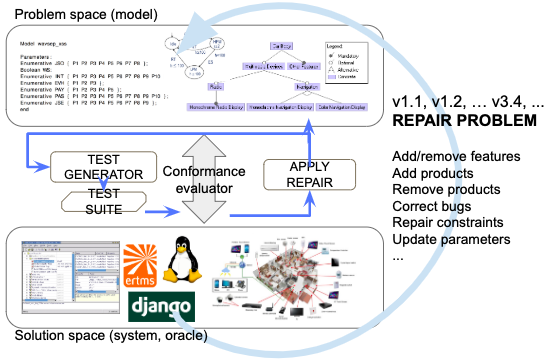
\includegraphics[width=.8\columnwidth]{images/repair.png}
	\caption{Test-Driven process to repair models}
	\label{fig:approach}
\end{figure}

%We plan to evaluate effectiveness and efficiency of the test-driven repair techniques on different applications, with real-world models and systems: from literature and from industrial cases. Apart from the already investigated applications to combinatorial and feature models, we plan to study a scenario of repair of 
%timed automata (TA), high order logic expressions, and finite state machines, for example. % they all have
%Timed automata are mainly used to describe the behavior of communication protocols, real-time systems and cyber-physical systems.
%The model could be abstracted to obtain parameters representing timing constraints in the guards or in the locations, resulting in a Parametric Timed Automata (PTA), and tests drive the detection of a configuration for such parameters, that reflects the \textit{updated} system.
%Each test, in this case, could be an \textit{execution trace}.%, that can happen or not in a given system, or according to the new specification.

%The dissemination plan consists in applying test-driven repair to real-world software systems, and possibly release tools, in addition to publishing papers to venues related to software testing or to the particular application for which test-driven repair has been applied.
%If real-world case studies coming from collaborations with industries in the sector are found, it would be an added value.


% in this part, there are the papers that do NOT focus on test generation, but start from UPDATE REQUEST, or FAILING COMBINATIONS
\chapter{Evolutionary Approach for Feature Model Repair}
Feature models are a widely used modeling notation for variability management in software product line (SPL) engineering. 
%In order to keep an SPL and its feature model aligned, feature models must be changed by including/excluding new features and products, either because faults in the model are found or to reflect the normal evolution of the SPL.
%Such changes can be complex and error-prone due to the size of the feature model.
%Therefore, 
We developed an approach that \textit{repairs} a feature model w.r.t. a given update request in the form of combinations representing a set of configurations to be accepted or rejected, that may be detected by \textit{failing} test cases, or directly by engineer domain knowledge. % from a change in the specification.
The method is based on an evolutionary algorithm that iteratively mutates the original feature models and checks if the update request is semantically fulfilled.
We employ mutations such as switching an optional feature to mandatory, or changing an \emph{or} group to an \emph{and} group, based on \cite{arcaini2018evolutionary}.
% \cite{arcaini2018evolutionary,ARCAINI201964}.
We generate faults between two real versions of feature models of the {\tt MobileMedia}, {\tt HelpSystem},  {\tt SmartHome}, and {\tt ERP\_SPL} systems in the SPLOT repository\footnote{\url{http://52.32.1.180:8080/SPLOT/feature_model_repository.html}}, and we notice that although our approach does not guarantee to completely update all the possible feature models, on average, around 89\% of requested changes are applied, with minimal edits.%, helping in preserving domain knowledge.

%\subsection{Test generation and fault localization}
%The process is driven by update configurations or failure-inducing combinations in the input parameters of the system, and black-box (in particular, combinatorial) test generation and fault detection and localization techniques, are important to support engineers in determining such inputs for the repair process.
%To this purpose, we make use of a tool to make it easier the editing of combinatorial models, and the test suite generation, called CTWedge \cite{IWCTGargantini2018}, and we devise a fault localization process, based on combinatorial testing, that guarantees to find the correct detection of failure-inducing combinations, under the assumption that the maximum strength of the real failure-inducing combinations is known.

\section{Basic definitions}\label{sec:basic}

\begin{tikzborder}{\cite{arcaini2018evolutionary}}
In software product line engineering, feature models are a special type of information model representing all possible products of an SPL in terms of features and relations among them. Specifically, a feature model \fm is a hierarchically arranged set of features $F$, where each parent-child relation between them is a constraint of one of the following types\footnote{As done by FeatureIDE~\cite{FeatureIDEbook}, we assume that each feature can be the father of only one group (either {\it Or}, {\it Alternative}, or {\it And}). This is not a limitation, as having different groups as children can be obtained by using abstract features~\cite{thum_abstract_2011}.}:
%
\begin{compactitem}
\item \textit{Or}: at least one of the sub-features must be selected if the parent is selected.
\item \textit{Alternative} (xor): exactly one of the children must be selected whenever the parent feature is selected.
\item \textit{And}: if the relation between a feature and its children is neither an \textit{Or} nor an \textit{Alternative}, it is called \textit{and}. Each child of an \textit{and} must be either:
\begin{compactitem}
\item \textit{Mandatory}: the child feature is selected whenever its respective parent feature is selected.
\item \textit{Optional}: the child feature may or may not be selected if its parent feature is selected.
\end{compactitem}
\end{compactitem}

Only one feature in $F$ has no parent and it is the \emph{root} of \fm.

In addition to the parental relations, it is possible to add \emph{cross-tree constraints}, i.e., relations that cross-cut hierarchy dependencies. {\it Simple} cross-tree constraints are:
%
\begin{compactitem}
\item A {\it requires} B: the selection of feature A in a product implies the selection of feature B. We also indicate it as $A \rightarrow B$.
\item A {\it excludes} B: A and B cannot be part of the same product. We also indicate it as $A \rightarrow \neg B$.
\end{compactitem}

Some frameworks for feature models also support {\it complex} cross-tree constraints~\cite{knuppel_is_2017} through {\it general} propositional formulas. In our approach, we allow feature models to contain complex cross-tree constraints.

Feature models can be visually represented by means of feature diagrams, and their semantics can be expressed by using propositional logic~\cite{batory2005feature,benavides2010automated}: features are represented by propositional variables, and relations among features by propositional formulae. We identify with $\fmToBool(\fm)$ the \textsc{BO}olean \textsc{F}ormula representing a feature model \fm.

\begin{mydef}[\textbf{Configuration}]\label{def:configuration}
A \emph{configuration} $c$ of a feature model \fm is a subset of the features $F$ of \fm (i.e., $c \subseteq F$).
\end{mydef}

If \fm has $n$ features, there are $2^n$ possible configurations.

\begin{mydef}[\textbf{Validity}]\label{def:validity}
Given a feature model \fm, a configuration $c$ is \emph{valid} if it contains the \emph{root} and respects the constraints of \fm. A valid configuration is called \emph{product}.
\end{mydef}

For our purposes, we exploit the propositional representation of feature models for giving an alternative definition of configuration as a set of $n$ literals $c = \{l_1, \ldots, l_n\}$ (with $n = |F|$), where a positive literal $l_i=f_i$ means that feature $f_i$ belongs to the configuration, while a negative literal $l_i=\neg f_i$ means that $f_i$ does not belong to the configuration. We will also represent a configuration as a BOolean Formula as follows: $\fmToBool(c) = \bigwedge_{i=1}^n l_i$.

Furthermore, since in the proposed approach we need to evaluate a feature model over a possibly wider set of features $U$, we introduce $\fmToBool(\fm, U) = \fmToBool(\fm) \wedge \bigwedge_{f \in U \setminus F} \neg f$, where \fm explicitly refuses all the configurations containing a feature not belonging to its set of features $F$; such technique has been already employed by different approaches that need to compare feature models defined over different sets of features~\cite{thum_reasoning_2009,icst2015}.

\begin{exmp}\label{ex:initialFM}
Let's consider the feature model shown in Fig.~\ref{fig:fmExample}.
%
\begin{figure}[!tb]
\centering
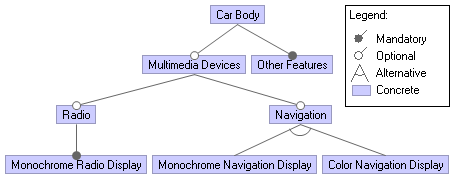
\includegraphics[height=3.5cm]{car2011}
\caption{Example of feature model (taken from~\cite{Pleuss2012})}
\label{fig:fmExample}
\end{figure}
%
It is the third version of the CAR SPL described in~\cite{Pleuss2012}. It is composed of eight features $F$ = \{\CarBody, \MultimediaDevices, \OtherFeatures, \Radio, \Navigation, \MonochromeRadioDisplay, \MonochromeNavigationDisplay, \ColorNavigationDisplay{}\}. \CarBody is the root feature; its children \MultimediaDevices and \OtherFeatures are respectively optional and mandatory. \MultimediaDevices has two optional children: \Radio that is the father of the mandatory feature \MonochromeRadioDisplay, and \Navigation that is the father of the alternative group between \MonochromeNavigationDisplay and \ColorNavigationDisplay.
\end{exmp}

\section{Specifying an update request}\label{sec:updateRequest}

We suppose that the product line engineer wants to update an existing feature model \initFm ({\it initial feature model}); although (s)he knows which are the desired updates in terms of products and features to add or remove, (s)he does not know how to write a feature model \fmp that satisfies all these updates.

In this section, we describe how the user can specify her/his {\it change requirements}.
By analysing existing evolutions of feature models described in literature~\cite{Pleuss2012,Burdek2016,smartHomePaper,helpSystemPaper,multimediaPaper}, we identified the following five types of change requirements: 
%
\begin{compactitem}
\item a feature must be identified with a new name. Although this change requirement is straightforward to achieve, it is widely used (e.g., for the Smart\-Home SPL~\cite{smartHomePaper} considered in the Ample Project, we have observed 12 feature renames) and it is important to keep track of it, otherwise someone reading the updated feature model may have the impression that one feature has been added and one removed (in particular, if also other changes have been done on the feature model and, therefore, spotting the renamed feature is not easy).
\item a feature must be added to the feature model. This change requirement occurs when a new feature must now be supported by the SPL. For example, in the CAR SPL~\cite{Pleuss2012}, the support for {\it DVD entertainment} has been introduced in 2012 (documented in the fourth version of the SPL feature model).
\item a feature must be removed from the feature model. This change requirement occurs when a feature is no more supported by the SPL.\footnote{Note that this change requirement could be achieved by removing all the products containing the feature (see last change requirement), but not removing the feature from the feature model. However, in this way, the feature would become {\it dead}~\cite{benavides2010automated}, making the feature model less readable.} For example, in the CAR SPL~\cite{Pleuss2012}, feature {\it Color Radio Display} has been removed in 2011 (third version of the SPL feature model).
\item some products must now be accepted by the SPL. This change requirement occurs when some constraints existing on the SPL (due to technical reasons or regulations) do not hold anymore and so some configurations that were forbidden in the past can now be accepted. For example, in the second version of the Pick-\&-Place (PPU) Unit SPL~\cite{Burdek2016}, the system is able to process either {\it plastic} or {\it metal} workpieces; in the third version of the SPL, instead, a technical improvement has allowed to handle plastic and metal workpieces in combination.
\item some products cannot be accepted anymore by the SPL. This change requirement happens when some constraints over the SPL emerge (e.g., due to new regulations). For example, in the {HelpSystem} SPL~\cite{helpSystemPaper}, the second version of the SPL does not allow anymore that the sensor only detects either {\it pressure} or {\it not pressure}, i.e., the products with only {\it pressure} or {\it not pressure} are not allowed and have been removed.
\end{compactitem}

In the following, we provide the formal definition of update request. We assume that the initial feature model does not contain any dead feature or redundant constraint~\cite{benavides2010automated,Duran2017FLAME}; in case it has any, we can remove them using standard techniques, as, for example, that provided by FeatureIDE~\cite{FeatureIDEbook}.

\begin{mydef}[\textbf{Update request}]\label{def:fic}
Given an initial feature model \initFm defined over a set of features $F$, we call \emph{update request} \UR the modifications a user wants to apply to \initFm in order to obtain the desired updated model \fmp. An update request is composed of five change requirements, three regarding the features of the feature model, and two the configurations/products. The first \emph{feature-based} change requirement regards the features names:
%
\begin{compactitem}
\item {\bf Rename features}: $\Ftbr = \{f_1,$ $\ldots,$ $f_m\}$ is a subset of features of $F$ that must be renamed and \rename a renaming function; \renamedFeatures is the set obtained by replacing every feature $f_i \in \Ftbr$ with $\mathit{ren}(f_i)$, i.e., $\renamedFeatures = (F \setminus \Ftbr) \cup \bigcup_{f_i \in \Ftbr} \{\rename(f_i)\}$. We identify with \fmrenamed the feature model obtained by renaming the features according to \Ftbr and \rename.\footnote{Note that feature renaming is already supported by feature model editors, such as FeatureIDE. We keep it among our change requirements for completeness with respect to the feature model evolutions observed in literature.}
\end{compactitem}
The other two \emph{feature-based} change requirements over the features of \fmrenamed are:
\begin{compactitem}
\item {\bf Add features}: \Fadd is a set of features the user wants to add to \fmrenamed. For each $e$ in \Fadd, the user has to define in $F_R \cup \Fadd$ the parent of $e$, denoted by \parent{e}. By adding a feature $e$ with parent $p$, we assume that the user wants to duplicate all the products that contain $p$ by adding also $e$.\footnote{Note that this corresponds to have $e$ as optional feature of $p$. However, this could not be always achievable, as explained in Sect.~\ref{sec:featBasedChangeReqs} (unless abstract features~\cite{thum_abstract_2011} are used); therefore, we define the change requirement in this more general form, in order to keep the semantics of change requirement and the way to achieve it clearly distinguished.} 
\item {\bf Remove features}: \Frem is a subset of the features of $F_R$ to remove; by removing a feature $f$, we assume that the user wants to remove $f$ from all the existing products and prohibit its selection in new products.
\end{compactitem}
%
We identify with $F^\prime$ the new set of features that must be used in the updated feature model \fmp, namely $(\renamedFeatures \cup \Fadd) \setminus \Frem$.

Two \emph{product-based} change requirements, instead, are related to the products/configurations of the feature model (over the new set of features $F^\prime$):
%
\begin{compactitem}
\item {\bf Add products}: \CFrelax is a set of predicates $\{ \rho_1, \ldots, \rho_n\}$ over $F^\prime$ that denote conditions that must be allowed in \fmp. The logical models satisfying $\rho_i$ are products that must be added to the feature model, provided that they do not violate feature model constraints defined over features not included in $\rho_i$.
\item {\bf Remove products}: \CFrem is a set of predicates $\{ \gamma_1 \ldots, \gamma_m\}$ over $F^\prime$ that denote a set of products to be removed. Each product (i.e., logical model) satisfying a $\gamma_i$ must be removed from the valid product set.
\end{compactitem}
\end{mydef}

The meaning of \CFrelax and \CFrem is to modify the set of valid products, as depicted in Fig.~\ref{fig:cremcrelax}.
%
\begin{figure}[tb!]
\begin{center}
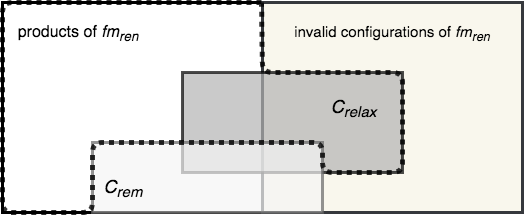
\includegraphics[width=.8\textwidth]{images/CremCrelax}
\end{center}
\caption{Added and removed products}
\label{fig:cremcrelax}
\end{figure}
%
The new product set (in dotted line) is enriched by configurations identified by \CFrelax but deprived of the products identified by \CFrem; note that \CFrem could also remove some products added by \CFrelax.

If the user wants to include/exclude a specific configuration $c$, then (s)he simply adds $\fmToBool(c)$ to \CFrelax/\CFrem.\footnote{This is what we actually do in the experiments in Sect.~\ref{sec:experiments} where update requests are computed as differences between different versions of feature models, and \CFrelax and \CFrem can only be identified in terms of sets of configurations.}



\subsection{Well-formedness of an update request}\label{sec:wfUpdReq}

We impose some constraints on the update request to be sure that the different change requirements are not contradictory and useful (i.e., they actually affect the product set):
%
\begin{compactenum}
\item \label{item:notCicleParentAndNotRemPar} Each added feature in \Fadd must have an ancestor in $\renamedFeatures\setminus\Frem$. This implies that it is not possible to remove by \Frem the parents $p$ of features added in \Fadd, i.e., $\Frem \cap (\bigcup_{f \in \Fadd} \{\parent{f}\}) = \emptyset$.
\item \label{item:notRemRen} It is not possible to remove features that have been renamed, i.e., $\Frem \cap (\bigcup_{f_i \in \Ftbr} \{\rename(f_i)\}) = \emptyset$.
\item \label{item:relaxNotRemFeat} Predicates in \CFrelax cannot predicate over features that have been removed in \Frem.
\item \label{item:relaxEffective} \CFrelax actually increases the set of products: for each $\rho_i$ in \CFrelax, there exists at least one non-valid configuration that satisfies $\rho_i$.
\item \label{item:remEffective} \CFrem actually deletes some products: for each $\gamma_i$ in \CFrem, there exists at least one product that satisfies $\gamma_i$.
\item \label{item:remNotBossy} \CFrem does not remove all the configurations that must be added by \CFrelax, i.e., for each $\rho_i$ and $\gamma_j$ there exists a configuration that satisfies $\rho_i$ (it must be added) and it does not satisfy $\gamma_j$.
\item \label{item:notIncons} The update request should be achievable by a consistent feature model (i.e., accepting at least one product) without dead features (i.e., each feature is selected in at least one model).
\end{compactenum}

Constraints
%\ref{item:notCicleParent}, \ref{item:notRemPar},
\ref{item:notCicleParentAndNotRemPar},
\ref{item:notRemRen}, and \ref{item:relaxNotRemFeat} can be easily checked directly at the syntactical level on the update request. If one of these constraints is not satisfied, the update request cannot be applied and we ask the user to fix it.

Checking constraints \ref{item:relaxEffective}, \ref{item:remEffective}, and \ref{item:remNotBossy}, instead, requires to reason over the propositional representation of \fmrenamed (i.e., $\fmToBool(\fmrenamed)$) and the predicates in \CFrelax and \CFrem; for example, checking constraint \ref{item:relaxEffective} consists in verifying that, for each $\rho_i \in \CFrelax$, $\neg \fmToBool(\fmrenamed) \wedge \rho_i$ is satisfiable. If one of these constraints is not satisfied, the update request is still consistent, although the corresponding change requirement is useless; in case of constraint violation, we warn the user about the useless change requirement and, if (s)he confirms that the change requirement is indeed not necessary, we continue the updating process without that requirement.

Checking constraint \ref{item:notIncons}, instead, requires to reason about the interaction of the different change requirements and can only be done after we define the target, as explained in the next section.

\begin{exmp}\label{ex:updReq}
Given the CAR SPL model shown in Fig.~\ref{fig:fmExample} and described in Ex.~\ref{ex:initialFM}, an update request could be the following\footnote{Note that the change requirement \Fadd is the same reported in~\cite{Pleuss2012} for the evolution from the third version (shown in Fig.~\ref{fig:fmExample}) to the fourth version of the CAR SPL; \CFrem, instead, is taken from the evolution from the first to the second version of the same SPL. In order to have a complete example, the other three change requirements have been identified by us; \Ftbr and \Frem resemble similar change requirements observed in literature, respectively in the SmartHome SPL~\cite{smartHomePaper} and in the CAR SPL~\cite{Pleuss2012}.}:
%
\begin{compactitem}
\item \textbf{Rename features} \Ftbr = \{\MonochromeRadioDisplay{}\} and \rename(\MonochromeRadioDisplay) = \RadioDisplay.
\item \textbf{Add features} \Fadd = \{\DVDEntertainment{}\} and \parent{\DVDEntertainment} = \MultimediaDevices.
\item \textbf{Remove features} \Frem = \{\OtherFeatures{}\}.
\item \textbf{Add products} \CFrelax = \{\MultimediaDevices $\wedge$ \Navigation $\wedge$ (\MonochromeNavigationDisplay $\leftrightarrow$ \ColorNavigationDisplay{})\}. We also want to allow products with support for navigation, and having both displays or having no display at all. 
\item \textbf{Remove products} \CFrem = \{$\Navigation \wedge \neg \Radio$\}. We want to exclude that navigation is present when the radio is not.
\end{compactitem}
\end{exmp}


\subsection{Update request semantics}\label{sec:target}

We here precisely define the semantics of an update request \UR. In order to do this, we define a formula that accepts and rejects configurations as the updated feature model should do.

In order to define the semantics of \Frem and \CFrelax, we need to be able to represent the feature model without some features. We exploit the approach used in~\cite{thum_abstract_2011} to remove features from feature models. To eliminate a feature $f$ from a propositional formula, we substitute $f$ by its possible values (true or false). 

\begin{mydef}[Features removal]\label{def:featuresRem}
Given a feature model \fm and a set of features $K = \{f_1,$ $\ldots,$ $f_k\}$ to remove, we recursively define $\filter(\fm, K)$ as follows:
%
\begin{equation*}
\filter(\fm, K) =\begin{cases}
\fmToBool(\fm) & {\rm if} \; K = \emptyset\\
\filter(\fm, K^\prime)[f \leftarrow \top] \vee \filter(\fm, K^\prime)[f \leftarrow \bot] & {\rm if} \; K = K^\prime \cup \{f\}\\
\end{cases}
\end{equation*}
%
\end{mydef}

The formula $\filter(\fm, K)$ has as logical models the same models as $\fmToBool(\fm)$ except that all the features in $K$ have been removed.

Exploiting Def.~\ref{def:featuresRem}, the semantics of \Frem is captured by the formula
%
\[\phi_{\mathit{rem}} = \filter(\fmrenamed, \Frem)\] 
%
whose logical models (i.e., products) are those of \fmrenamed without the removed features.

In order to capture the semantics of a $\rho_i \in \CFrelax$, we need to characterize the set of configurations to add. These are those that satisfy $\rho_i$ but still respect the constraints of $\phi_{\mathit{rem}}$, except for those involving the features of $\rho_i$. This is captured by
%
\[\phi^i_{\mathit{relax}} = \filter(\phi_{\mathit{rem}}, \mathit{features}(\rho_i)) \wedge \rho_i\]
%
being $\mathit{features}$ a function returning the features (i.e., propositional variables) contained in a formula. The {\it filter} on $\phi_{\mathit{rem}}$ has the effect of making the features in $\rho_i$ unconstrained, i.e., it keeps only the constraints of $\phi_{\mathit{rem}}$ that do not {\it interfere} with $\rho_i$.

We can now build the formula that defines the semantics of the whole update request. We name the formula as {\it target} as it will be used as oracle to guide the proposed updating process (see Sect.~\ref{sec:process}).

\begin{mydef}[\textbf{Target}]\label{def:target}
The target $t$ is a propositional formula whose models exactly correspond to the products of the desired updated feature model. Assume an update request $\UR = \{\rename, \parentna, \Frem, \CFrelax, \CFrem{}\}$ defined over a feature model \fm, with the functions \rename defined over \Ftbr and \parentna defined over \Fadd. Let \fmrenamed be the feature model renamed according to \rename; the target is defined as:
%
\begin{align*} 
t = & (\overbrace{\;\phi_{\mathit{rem}}\;}^{\parbox{18mm}{\footnotesize remove \Frem\\from products}} \vee \overbrace{\bigvee_{\rho_i \in \CFrelax} \phi^i_{\mathit{relax}}}^{\parbox{17mm}{\footnotesize add products}}) & \wedge
& \overbrace{\bigwedge_{f \in \Fadd} f \rightarrow \parent{f}}^{\parbox{24mm}{\footnotesize add \Fadd features only when possible}} \wedge \overbrace{\bigwedge_{f \in \Frem} \neg f}^{\parbox{17mm}{\footnotesize disable \Frem\\ features}} \wedge \overbrace{\bigwedge_{\gamma \in \CFrem} \neg \gamma}^{\parbox{12mm}{\footnotesize remove products}}
\end{align*}
\end{mydef}

The target correctly rejects all the configurations of \CFrem and those containing a removed feature in \Frem; the accepted configurations are those in \CFrelax, plus those of $\phi_{\mathit{rem}}$ (i.e., the original feature model without the removed features) possibly extended with each added feature $f$ of \Fadd only when \parent{f} is present.

Note that the target correctly predicates over all the features $F_U = F^\prime \cup \Frem$: those of the original feature model (after renaming), those added, and those removed.

\paragraph{Checking the target}
On the target, we can finally check constraint \ref{item:notIncons} described in Sect.~\ref{sec:wfUpdReq}, requiring that the update request does not produce anomalies.

First of all, we check that the target accepts at least one product (i.e., it is satisfiable); if not, we warn the user that the update request cannot be applied.

Moreover, we also check that each feature $f \in F^\prime$ can be actually selected in at least one product; it this is not possible, it means that $f$ is required to be dead in the final model. If this is the case, we warn the user about this and, if this is the intended behavior, we move $f$ in \Frem, so that we can directly try to remove it during the repairing process.


\section{Evolutionary updating process}\label{sec:process}

Modifying the initial feature model \initFm such that it satisfies the update request as specified by the target is a challenging task. Note that, in general, there could be no \fmp that exactly adds and removes the specified configurations and features, unless {\it complex} cross-tree constraints are used. However, we claim that the usage of these constraints should be discouraged. Urli et al.~\cite{visualSupport} observe that ``they make FMs complex to understand and maintain'', Reinhartz-Berger et al.~\cite{ComprehendingFeatureModels} experimentally assessed that they are more difficult to understand than parent-child relationships (at least, by modelers who are unfamiliar with feature modeling), and Berger et al.~\cite{Berger2013} report that ``they are known to critically influence reasoners''. Also the authors of FeatureIDE noted that cross-tree constraints ``are harder to comprehend than simple tree constraints" and that ``relations among features should be rather expressed using the tree structure if possible''~\cite{FeatureIDEbook}. In this paper, we therefore avoid the addition of complex cross-tree constraints, as we not only aim at correctness (i.e., full achievement of the update request), but also at readability of the final model.
Some approaches that aim at simplifying complex constraints exist~\cite{knuppel_is_2017,vonRhein2015}, but they may diminish readability and other qualities, such as compactness, traceability, and maintainability.\footnote{In Sect.~\ref{sec:conclusions}, we discuss how complex cross-tree constraints could be used to achieve all the change requirements and the issues that could be related to that approach.}

This paper proposes a heuristic approach that tries to achieve the update request {\it as much as possible}. In order to do this, we use the target as {\it oracle} to compute the {\it fault ratio}. The fault ratio tells how close we are to the correct solution. In Sect.~\ref{sec:correctness}, we give the definition of fault ratio and then, in Sect.~\ref{sec:updatingProcess}, we describe the updating process we propose.

\subsection{Correctness}\label{sec:correctness}

We can use the target to evaluate whether a feature model \fmp captures the desired change requirements, i.e., \fmp is equivalent to the target ($\models t \leftrightarrow \fmToBool(\fmp, F_U)$). In the following, we will only compare feature models \fmp whose features $F_{\fmp}$ are, at most, those in $F_U$, i.e., $F_{\fmp} \subseteq F_U$.

Although a feature model could not fulfill all the change requirements, it could satisfy them partially. We give a measure of the \emph{difference} between a feature model \fm (either the initial one \initFm or a modified one \fmp) and the target as follows.

\begin{mydef}[\textbf{Fault ratio}]\label{def:faultratio}
Given a feature model \fm and a target $t$, the \emph{fault ratio} of \fm w.r.t. $t$ is defined as follows:
%
\begin{equation*}
\FR(\fm, t) = \frac{|\mathit{AllConfs}(\fmToBool(\fm, F_U) \neq t, F_U)|}{2^{|F_U|}}
\end{equation*}
%
where $\mathit{AllConfs}(\varphi, V)$ returns all the logical models of formula $\varphi$, i.e., all the truth assignments $m$ to propositional variables $V$, such that $m \models \varphi$.\footnote{In our approach, we represent formulas as Binary Decision Diagrams (BDDs) in JavaBDD that implements $|\mathit{AllConfs}|$ by means of the method $\mathtt{satCount}$ that directly computes the cardinality of the set without enumerating all the models.}
\end{mydef}

If the fault ratio is equal to 0, it means that \fm accepts as products the same configurations that are logical models of $t$; otherwise, there are some configurations that are wrongly evaluated by \fm, as shown in Fig.~\ref{fig:faults}: \fm could wrongly accept some configurations and/or wrongly refuse some others.
%
\begin{figure}[!tb]
\def\languageAll{(-1.2,-1.2) rectangle (2.2cm,1.2cm)}
\def\firstcircle{(0,0) circle (1cm)}
\def\circleS{(0:1cm) circle (1cm)}
\colorlet{circle edge}{black}
\tikzset{
filled1/.style={draw=circle edge},
filled2/.style={pattern=north east lines, pattern color=gray},
outline/.style={draw=circle edge, thick}}
\centering
\begin{tikzpicture}
\begin{scope}
\draw[filled2, even odd rule] \firstcircle \circleS;
\end{scope}
\begin{scope}
\end{scope}
\draw[outline] \firstcircle node [left=0mm] {\fm};
\draw[outline] \circleS node [right=2mm] {$t$};
\draw[outline] \languageAll node [right=0mm] {$2^{\mid F_U\mid}$};
\begin{customlegend}[legend cell align=left, %<= to align cells
legend entries={ % <= in the following there are the entries
{correct configurations}, 
{wrong configurations}
},
legend style={at={(6.5, 0.5)},font=\footnotesize}] % <= to define position and font legend
% the following are the "images" and numbers in the legend
\addlegendimage{area legend,filled1}
\addlegendimage{area legend,filled2}
\end{customlegend}
\end{tikzpicture}
\caption{Faults}
\label{fig:faults}
\end{figure}

\begin{exmp}
Fig.~\ref{fig:exampleUpdatedFM} shows a possible updated model that exactly satisfies all the change requirements reported in Ex.~\ref{ex:updReq} for the model in Fig.~\ref{fig:fmExample}.
%
\begin{figure}[tb!]
\centering
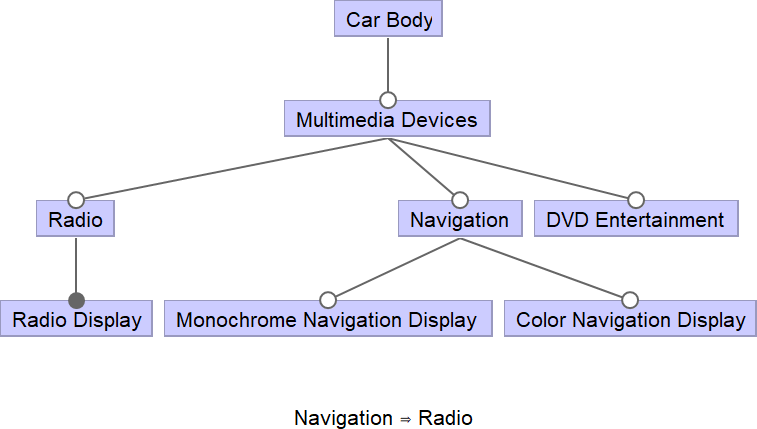
\includegraphics[height=5cm]{car2011_4paper}
\caption{Updated feature model}
\label{fig:exampleUpdatedFM}
\end{figure}
%
Note that the fault ratio of the initial renamed feature model \initFm w.r.t. to the target $t$ (that corresponds to the final feature model) is $\frac{20}{2^9}$, as \initFm wrongly accepts all its 7 products and wrongly rejects all the 13 products of the target.
\end{exmp}


\subsection{Updating process}\label{sec:updatingProcess}

The process we propose to update an initial feature model \initFm, given an update request \UR, is depicted in Fig.~\ref{fig:approach}.
%
\begin{figure*}[!tb]
\centering
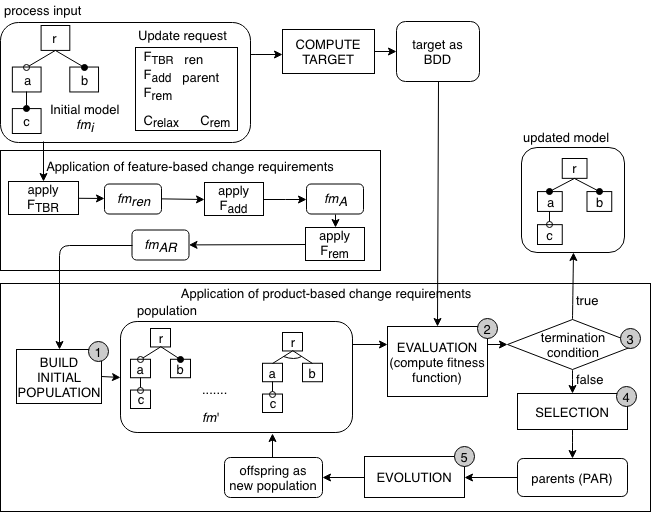
\includegraphics[width=\textwidth]{evolutionaryApproach}
\caption{Proposed evolutionary approach}
\label{fig:approach}
\end{figure*}
%
As initial step, we generate the target $t$ as a Binary Decision Diagram (BDD), as described in Def.~\ref{def:target}. Then, we start the updating process, that is composed of two consecutive macro-phases. We first try to deal with the feature-based change requirements (see Sect.~\ref{sec:featBasedChangeReqs}) and then with the product-based ones (see Sect.~\ref{sec:prodBasedChangeReqs}).

\subsubsection{Dealing with feature-based change requirements}\label{sec:featBasedChangeReqs}

First of all, we apply \Ftbr to rename features, obtaining the feature model \fmrenamed.

Then, we modify \fmrenamed in order to try to achieve the change requirements of \Fadd and \Frem. For each $f \in \Fadd$, we add $f$ as child of \parent{f} as follows: if \parent{f} is the father of an {\it Or} or an {\it Alternative} group, $f$ is added to the group; in all the other cases, it is added as {\it Optional} child of \parent{f}. We name as $\fm_{A}$ the feature model obtained after this step. Then, for each feature $f \in \Frem$, $f$ is removed from $\fm_{A}$ and replaced by its children $\mathit{Ch_f}$ (if any). The relation of the moved children $\mathit{Ch_f}$ of $f$ with their new parent $p$ is set according to the way FeatureIDE removes features~\cite{FeatureIDEbook}:
%
\begin{compactenum}
\item If $f$ was the only child of $p$, $p$ takes the group type of $f$. 
\item If $p$ has group type {\it And}, 
\begin{inparaenum}
\item if the children $\mathit{Ch_f}$ are in {\it And} relationship, they keep their type (either {\it Mandatory} or {\it Optional})
\item otherwise (they are in {\it Alternative} or {\it Or}), they are set to {\it Optional}.
\end{inparaenum}
\item Otherwise, if $p$ has group type {\it Alternative} or {\it Or}, features in $\mathit{Ch_f}$ are simply added to the group (regardless of their type).
\end{compactenum}


We name as $\fm_{\mathit{AR}}$ the feature model obtained after this step.

Note that the model $\fm_{\mathit{AR}}$ could still be not equivalent to the target, i.e., $\not \models t = \fmToBool(\fm_{\mathit{AR}}, F_U)$. This could be due to two reasons. First of all, the update request could also require to add as products configurations described by constraints in \CFrelax and/or remove configurations described by constraints in \CFrem. Moreover, the two previous transformations do not guarantee to precisely implement the required change requirements \Fadd and \Frem, and they could introduce some wrong configurations (either wrongly accepted or rejected). For example, in order to implement the addition of a feature $f$ with $\parent{f} = p$ and $p$ father of an alternative group, we add $f$ to the group; however, this is not the exact semantics of \Fadd that requires to duplicate the products containing $p$ and adding $f$ to them.


\subsubsection{Dealing with product-based change requirements}\label{sec:prodBasedChangeReqs}

Starting from $\fm_{\mathit{AR}}$, we apply an evolutionary updating approach to try to obtain an updated feature model equivalent to the target. The process is an instance of classical evolutionary algorithms~\cite{Eiben2003}; an evolutionary algorithm can be understood (in a metaphor-free language~\cite{metaheuristicsMetaphor}) as an optimization problem in which different solutions are modified by random changes and their quality is checked by an objective function. Precisely, the steps are as follows:
%
\begin{compactenum}
\item \textbf{Initial population}: at the beginning, a population $P$ is created. $P$ is a set of candidate solutions.
\item \textbf{Iteration}: the following steps are repeatedly executed:
\begin{compactenum}
\item \textbf{Evaluation}: each member of the population $P$ is evaluated using a given \emph{fitness function}, representing the objective function.
\item \textbf{Termination}: a termination condition is checked in order to decide whether to start the next iteration. If the termination condition holds, the candidate with the best \emph{fitness value} is returned as final model.
\item \textbf{Selection} (\emph{Survival of the Fittest}): some members of $P$ having the best values of the fitness function are selected as parents of the next generation and collected in the set \PAR.
\item \textbf{Evolution}: parents \PAR are mutated to obtain the \emph{offspring} to be used as population in the next iteration. The mutation performs random changes suitable to improve the existing solutions.
\end{compactenum}
\end{compactenum}

In our approach, we assume that the population $P$ is a multiset (i.e., possibly containing duplicated elements) with fixed size $M$ equal to $H \cdot |F^\prime|$, where $H$ is a parameter of the process. In the following, we describe each step in details.


\paragraph{\bf Initial population}%\label{sec:initPopulation}

As initial population, we generate the set $P$ by cloning $\fm_{\mathit{AR}}$ $M$ times (step 1 in Fig.~\ref{fig:approach}). In this way, if $\fm_{\mathit{AR}}$ is already correct, it will be returned as final model in the \emph{termination condition} phase.

\paragraph{\bf Evaluation}%\label{sec:evaluation}
As first step of each iteration (step 2 in Fig.~\ref{fig:approach}), each candidate member \fmp of the population $P$ is evaluated using a \emph{fitness function} that tells how \emph{good} the member is in achieving the overall goal. We define the fitness function both in terms of fault ratio (see Def.~\ref{def:faultratio}) and of {\it complexity} of the model structure. Indeed, we would like to avoid that, during the updating process, the feature model becomes unreadable, unnecessarily complex, and difficult to maintain~\cite{Berger2013,visualSupport,ComprehendingFeatureModels,FeatureIDEbook}. We have decided to consider, at least initially, the number of cross-tree constraints as indicator of complexity, since the constraints among features should be expressed by structural relationships and cross-tree constraints should be used only when really necessary. We introduce the following fitness function:
%
\begin{equation}\label{eq:fitness}
\fitness(\fmp) = 1 - \FR(\fmp, t) - k \times \mathit{ctc}(\fmp)
\end{equation}
%
where $\mathit{ctc}$ is a function returning the number of cross-tree constraints of a feature model and $k$ a constant. In our approach, the quality of a candidate must be mainly given by the percentage of configurations that it evaluates correctly, i.e., $1 - \FR(\fmp, t)$; if a candidate $c_1$ evaluates correctly more configurations than a candidate $c_2$, its fitness should be guaranteed to be greater than that of $c_2$. However, for models having the same fault ratio, the fitness should penalize those that are structurally more complex. In order to obtain this effect, we use as $k$:
%
\begin{equation}\label{eq:kFitness}
k = \frac{1}{{2^{|F_U|} \times 2|F_U|^2}}
\end{equation}

Note that $2 |F_U|^2$ is a safe strict upper bound on the number of cross-tree constraints among the features of the feature model. Indeed, among the possible $2|F_U|^2$ cross-tree constraints, some of them are not introduced because redundant (e.g., two {\it excludes} constraints between $(a,b)$ and $(b,a)$ are redundant and only one is necessary). Therefore, the term $\frac{\mathit{ctc}(\fmp)}{2^{|F_U|} \times 2|F_U|^2}$ is guaranteed to be less than $\frac{1}{2^{|F_U|}}$ that is the minimal possible variation of the fault ratio due to the change of evaluation of a single configuration. This means that the term can only affect the ranking of feature models having the same fault ratio.


\paragraph{\bf Termination condition}%\label{sec:termination}
In this step (step 3 in Fig.~\ref{fig:approach}), the process checks whether at least one of the following conditions is met:
%
\begin{compactitem}
\item a defined level of fitness \thF is reached, i.e., there exists an \fmp in $P$ with $\fitness(\fmp) \ge \thF$. For example, $\thF=1$ means that we want to obtain a completely correct model without any cross-tree constraint; with $\thF = 1 - \frac{1}{2^{|F_U|} + 1}$, instead, we still want to have a correct model, but we allow to have any number of cross-tree constraints;
\item in the previous \thNI iterations there has been no improvement of the fitness value of the best candidate;
\item a maximum number \thI of iterations have been executed;
\item a total time threshold \thT has been reached.
\end{compactitem}

If at least one of the previous conditions holds, the \fmp in $P$ with the highest fitness value is returned as final model.\footnote{If there is more than one model with the highest fitness value, we randomly select one of these models.}


\paragraph{\bf Selection}%\label{sec:selection}

In the \emph{selection} step (step 4 in Fig.~\ref{fig:approach}), starting from population $P$, a multiset of \emph{parents} \PAR of size $p$ is built, being $p$ a parameter of the evolutionary process. Different selection strategies have been proposed in literature:
%
\begin{compactitem}
\item \emph{Truncation}: it selects the first $n = \left\lceil K\cdot|P| \right\rceil$ members of the population with the highest fitness value, where $K$ is a parameter specifying a percentage of the population ($0 < K \le 1$). Then, the first $n$ elements are added to \PAR as many times as necessary to reach the size $p$. Such strategy could result in premature convergence, as candidates with lower fitness values are not given the opportunity to improve their fitness.
\item \emph{Roulette wheel}: $p$ members of the population are selected randomly; each member can be selected with a probability proportional to its fitness value. Note that one or more individuals could be selected multiple times.
\item \emph{Rank}: it is similar to roulette wheel, except that the selection probability is proportional to the relative fitness rather than the absolute fitness, i.e., the probability of selecting a member is inversely proportional to its ranking number (where the member with highest fitness has ranking number 1). This strategy tends to avoid premature convergence by mitigating the selection pressure that comes from large differences in fitness values (as it happens in truncation selection).
\end{compactitem}


\paragraph{\bf Evolution}%\label{sec:evolution}
In the \emph{evolution} step (step 5 in Fig.~\ref{fig:approach}), the parents \PAR are used to generate the \emph{offspring} that constitutes the population of the next generation.

The idea we assume here is that the feature model should be updated applying a limited number of mutations. Making updates through the use of mutation operators has the benefit of reducing the risk of loss of domain knowledge, by changing the feature model as less as possible. Note that this assumption is similar to the competent programmer hypothesis~\cite{surveyMutationTesting} that assumes that the user has defined the artifact close to the correct one. If our approach is used for removing faults, we can directly rely on the competent programmer hypothesis. On the other hand, if the approach is used to evolve the feature model to align it with the SPL, we can still assume that the mutation operators are sufficient to obtain the updated model; indeed, it is unlikely that the updated version of the feature model should be too different from the initial one.

In order to build the next population $P$, we mutate all the feature models in \PAR using the operators presented in Table~\ref{tab:mutOperators}.
%
\begin{table}[!tb]
\caption{Mutation operators}
\resizebox{\textwidth}{!}{%
\centering
\begin{tabular}{rl}
\toprule
Name & Description\\
\midrule
\OptToMan & an {\it optional} feature is changed to {\it mandatory}\\
\ManToOpt & a {\it mandatory} feature is changed to {\it optional}\\
\OrToAl & an {\it or} group is changed to {\it alternative}\\
\OrToAnd & an {\it or} group is changed to {\it and} with all children {\it mandatory}\\
\OrToAndOpt & an {\it or} group is changed to {\it and} with all children {\it optional}\\
\AlToOr & an {\it alternative} group is changed to {\it or}\\
\AlToAnd & an {\it alternative} group is changed to {\it and} with all children {\it mandatory}\\
\AlToAndOpt & an {\it alternative} group is changed to {\it and} with all children {\it optional}\\
\AndToAl & an {\it and} group is changed to {\it alternative}\\
\AndToOr & an {\it and} group is changed to {\it or}\\
\midrule
\PullUp & a feature is moved as sibling of its parent\\
\PushDown & a feature is moved as child of one of its siblings\\
\PullUpChildren & all children of a feature are moved as siblings of their parent\\
\PushDownSiblings & all siblings of a feature are moved as children of that feature\\
\midrule
\DelConstr & a cross-tree constraint ({\it requires} or {\it excludes}) is deleted\\
\ReqToExcl & a {\it requires} constraint is changed to an {\it excludes} constraint\\
\ExclToReq & an {\it excludes} constraint is changed to a {\it requires} constraint\\
\Creq & a {\it requires} constraint is created\\
\Cexc & an {\it excludes} constraint is created\\
\bottomrule
\end{tabular}}
\label{tab:mutOperators}
\end{table}
%
We set an upper bound $M$ to the size of the new population. If the mutation operators generate a maximum of $M$ mutants, we take all of them as the new population, otherwise we randomly select $M$ of them. In our approach, the offspring replaces the entire population.

{\it Description of mutation operators}
In~\cite{icst2015}, we have proposed some mutation operators for feature models, divided in \textit{feature-based} and \textit{constraint-based} operators that are a subset of the edit operations identified in~\cite{Burdek2016}. We use eight of the feature-based mutation operators proposed in~\cite{icst2015}, and introduce two new ones (\OrToAndOpt and \AlToAndOpt) that provide slightly different versions of \OrToAnd and \AlToAnd. Moreover, we also introduce two operators that permit to move a feature as sibling of the parent (\PullUp) or as child of one its siblings (\PushDown); we also introduce two versions of these operators that move all the children of a feature (\PullUpChildren) and all the siblings of a feature (\PushDownSiblings). Note that we do not allow the movement of a feature in any part of the feature model as this would produce too many mutants and could change too much the structure of the feature model. However, if in order to obtain the correct feature model a feature should be moved {\it far} from its current position, this is still obtainable by a suitable sequence of \PullUp and \PushDown mutations.

Finally, we use all the \textit{constraint-based} operators\footnote{Note that the mutation operator \DelConstr corresponds to operator \MC described in~\cite{icst2015}.} proposed in~\cite{icst2015}, and introduce two new ones (\Creq, \Cexc) to create {\it requires} and {\it excludes} constraints; in order to limit the number of generated mutants, we only create constraints among features that belong to different sub-trees of the feature model, i.e., neither feature of the constraint is ancestor of the other. Moreover, we avoid to create constraints that would be redundant or that would introduce dead features: for instance, $A \rightarrow \neg B$ is not added if $A \rightarrow B$ is already present in the model, because A would become a dead feature.

Although we allow feature models with constraints also in general form, we decided to not modify them, nor introduce new ones, in order to avoid the introduction of too many mutants and to achieve better readability of the final model.

In general, we cannot evaluate a priori if a mutant introduces an anomaly; therefore, for each mutant, we check if it is infeasible, it contains redundant constraints, or it has dead features. If it has any of these anomalies, we do not select it.



\section{Experiments}\label{sec:experiments}

The process\footnote{The code is available at \url{https://github.com/fmselab/eafmupdate}} has been implemented in Java by using Watchmaker\footnote{\url{https://watchmaker.uncommons.org/}} as evolutionary framework, FeatureIDE~\cite{FeatureIDEbook} to represent and mutate feature models, and JavaBDD for BDDs manipulation. 

We conducted a set of experiments to evaluate the proposed evolutionary approach; they have been executed on a Windows 10 system with an Intel i7-3770 3.40GHz processor, and 16 GB RAM.


\subsection{Benchmarks}\label{sec:benchmarks}

For the experiments, we used two sets of benchmarks, both shown in Table~\ref{tab:benchmarks}.
%
\begin{table}[!tb]
\caption{Benchmark properties}
\centering
\resizebox{\columnwidth}{!}{%
\begin{tabular}{clcc|ccccc} 
\toprule
& & \multicolumn{2}{c|}{model size} & \multicolumn{5}{c}{\UR size}\\
& SPL & input & target & $\vert \Ftbr \vert$ & $\vert \Fadd \vert$ & $\vert \Frem \vert$ & $\vert \CFrelax \vert$ & $\vert \CFrem \vert$\\
\midrule
\multirow{12}*{\rotatebox{90}{\small \benchReal}}
&{\tt MobileMedia d1} (V5..8) & 18.7 (15-23) & 22.3 (18-26) & 11.3 (1-17) & 4 (3-5) & 0.33 (0-1) & 26.7 (0-48) & 258 (24-560) \\
&{\tt MobileMedia d2} (V5..8) & 16.5 (15-18) & 24.5 (23-26) & 12 (11-13) & 8 (8-8) & 0 (0-0) & 64 (48-80) & 536 (528-544) \\
&{\tt MobileMedia d3} (V5,V8) &15 & 26 & 9 & 11 & 0 & 80 & 1648 \\
&{\tt HelpSystem} (V1, V2) & 25 & 26 & 0 & 1 & 0 & 672 & 2016 \\
&{\tt SmartHome} (V2.0, V2.2) & 39 & 60 & 12 & 23 & 2 & $1.92 \times 10^{9}$ & $2.31 \times 10^{10}$ \\
&{\tt ERP\_SPL} (V1, V2) & 43 & 58 & 0 & 15 & 0 & 0 & $1.51 \times 10^{7}$ \\
&{\tt PPU d1} (V1..9) & 13.9 (9-17) & 14.9 (11-17) & 0 (0-0) & 1.13 (0-4) & 0.125 (0-1) & 3.75 (0-27) & 27.8 (0-183) \\
&{\tt PPU d2} (V1..9) & 13.4 (9-17) & 15.4 (11-17) & 0 (0-0) & 2.14 (0-6) & 0.142 (0-1) & 9 (0-27) & 54.4 (0-243) \\
&{\tt PPU d3} (V1..9) & 12.8 (9-17) & 16.2 (13-17) & 0 (0-0) & 3.5 (1-6) & 0.167 (0-1) & 16 (0-27) & 77.5 (9-156) \\
&{\tt CAR d1} (V2009..2012) & 7 (6-8) & 9.33 (7-13) & 0 (0-0) & 2.67 (1-5) & 0.333 (0-1) & 5 (0-13) & 16 (1-40) \\
&{\tt CAR d2} (V2009..2012) & 6.5 (6-7) & 10.5 (8-13) & 0 (0-0) & 4.5 (3-6) & 0.5 (0-1) & 6 (0-12) & 34 (9-59) \\
&{\tt CAR d3} (V2009,V2012) & 6 & 13 & 0 & 7 & 0 & 0 & 87 \\
\midrule
\multirow{4}*{\rotatebox{90}{\small \benchMut}}
%& {\tt Example} & 4 & 4 & 0 & 0 & 0 & 0.41 (0-2) & 0.68 (0-2)\\
& {\tt Register} & 11 & 11 & 0 & 0 & 0 & 11.85 (0-40) & 62.28 (0-210)\\
& {\tt Graph} & 6 & 6 & 0 & 0 & 0 & 12.71 (0-28) & 0 (0-0)\\
&{\tt Aircraft} & 13 & 13 & 0 & 0 & 0 & 196.86 (0-315) & 53.53 (0-365)\\
& {\tt Connector} & 20 & 20 & 0 & 0 & 0 & 8.23 (0-18) & 26.02 (0-336)\\
\bottomrule
\end{tabular}
}
\label{tab:benchmarks}
\end{table}

\paragraph{Real models}
The first benchmark set \benchReal is constituted by SPLs described in literature for which different versions of their feature model have been developed. First, we have identified in the SPLOT repository\footnote{\url{http://52.32.1.180:8080/SPLOT/feature_model_repository.html}} four SPLs that evolved over time:
%
\begin{compactitem}
\item {\tt MobileMedia}: a program to manipulate multimedia on mobile devices (four versions)~\cite{multimediaPaper};
\item {\tt HelpSystem}: a cyber-physical system with multiple sensors (two versions)~\cite{helpSystemPaper};
\item {\tt SmartHome}: a set of smart house components (two versions)~\cite{smartHomePaper};
\item {\tt ERP\_SPL}: an Enterprise Resource Planner (two versions).
\end{compactitem}
%
Then, we have also considered the industrial case of a Pick-and-Place Unit ({\tt PPU})~\cite{Burdek2016}; for this system, the feature model has been changed eight times to adapt to new requirements (therefore, there are nine feature models available~\cite{Burdek2016}). Finally, we have also considered the product line model of a {\tt CAR}~\cite{Pleuss2012}, for which four different feature models have been produced.

For each SPL, we identified couples (\initFm, $\fm_t$) of their feature models: the latest version was considered as target model\footnote{Note that, in the real usage of our approach, we do not have a target feature model, but an update request \UR from which we generate the target as propositional formula.} $\fm_t$, and the oldest one as the initial model \initFm we want to update. For SPLs with more than two feature models, in addition to couples of feature models of consecutive versions, we also considered models with version distance 2 and 3 (in the table, d1, d2, and d3 indicate the distance). In this way, we attempt to reproduce update requests of different complexity. In total, \benchReal contains 36 couples of models.

\paragraph{Generated models}
The second benchmark set \benchMut has been built with the aim of evaluating our approach under the assumption we did in Sect.~\ref{sec:prodBasedChangeReqs} that mutation operators are sufficient to update the feature model. We selected four feature models developed for four SPLs (for which only one model is available):
%
\begin{compactitem}
\item {\tt Register}: a register of supermarkets, adapted from~\cite{Shimbara2015};
\item {\tt Graph}: a graph library;
\item {\tt Aircraft}: the configurations of the wing, the engine, and the materials of airplane models;
\item {\tt Connector}: IP connection configurations.
\end{compactitem}
%
From these models (used as target models $\fm_t$), we automatically generated other versions to be used as input models \initFm; we randomly mutated the target models (using 1 to 10 mutations), applying the operators described in Table~\ref{tab:mutOperators}. For each target model, we generated 100 input models. Therefore, \benchMut contains 400 couples.

\subsubsection{Deriving the update request}
In the devised usage of the approach, the user should specify the update request that must be provided as input to the evolutionary process; however, for our experiments, we do not have any update request available. Therefore, we automatically generated an update request \UR from the initial feature model \initFm and the target feature model $\fm_t$ of each couple (\initFm, $\fm_t$) of the benchmarks.

In order to detect renamed features in \Ftbr, we manually inspected the two feature models and produced the renamed model \fmrenamed. Then, from \fmrenamed and $\fm_t$, we automatically identified the differences of their features for building \Fadd and \Frem; moreover, using their BDD representation, we identified the configurations that are differently evaluated in order to build \CFrelax and \CFrem (we built a predicate for each wrongly evaluated configuration\footnote{Note that, in this way, the sets \CFrelax and \CFrem are very large because they contain a predicate for each added and removed configuration. However, in a real setting, the user should specify predicates capturing sets of configurations and so the sets should be much smaller.}). Note that configurations that are added and removed by \Fadd and \Frem are not also specified in \CFrelax and \CFrem.

Table~\ref{tab:benchmarks} reports, for all the benchmarks, the size of the input and target models in terms of number of features, and the number of requirements of the update request. For the SPLs in \benchReal having more than one couple of feature models, the reported values are aggregated by distance; for each SPL in \benchMut, the values are aggregated among its 100 input models. For these aggregated models, we report the average, minimum, and maximum number of elements in the update request. In \benchMut, since we did not add or remove features for producing the input models, their size is the same of that of the target model and so \Fadd and \Frem are empty; moreover, we do not even rename features and so also \Ftbr is empty.



\subsection{Analysis}\label{sec:analysis}

We now evaluate the proposed approach by a series of research questions. In these experiments, we set the parameters of the termination conditions as follows: \thF to $1 - \frac{\mathit{ctc}(\initFm)}{{2^{|F_U|} \times 2|F_U|^2}}$, \thNI to 15, \thI to 25, and \thT to 30 minutes. Note that the value chosen for \thF requires to have a totally correct model, with at most the same number of cross-tree constraints of the starting feature model. The parameter $H$ used to determine the maximum population size $M$ (as defined in Sect.~\ref{sec:prodBasedChangeReqs}) has been set to 5, and the parameter $p$ of the selection phase has been set to $\nicefrac{M}{2}$. All the reported data are the averages of 30 runs.

In~\cite{evolUpdateVAMOS2018}, we experimented the effect of the different selection policies of the evolutionary approach and we found that truncation with $K$=5\% is the best policy in terms of fault ratio reduction, and the second best as execution time. Therefore, we here select it as selection policy and evaluate the approach using other research questions.

\researchquestion{Is the proposed approach able to achieve the change requirements specified by the update request?}

For each benchmark SPL, Table~\ref{tab:processPerformance} reports (among other things) the initial and final values of \FR, and the \FR reduction.
%
\begin{table}[!tb]
\caption{Performance of the updating process}
\resizebox{\textwidth}{!}{%
\centering
\setlength\tabcolsep{2pt} 
\begin{tabular}{c l rrrrrrrrr}
\toprule
& SPL & \shortstack{time\\(s)} & \shortstack{initial\\FR (\%)} & \shortstack{final\\FR (\%)} & \shortstack{FR\\reduction (\%)} & \shortstack{\# \\ iterations} & \shortstack{sem.\\eq. (\%)} & \shortstack{synt.\\eq. (\%)} & ctc & ED \\
\midrule
\multirow{12}*{\rotatebox{90}{\small \benchReal}} &   {\tt MobileMedia d1}  & 71.11 &  4.17e-03 & 1.10e-04 & 96.03 & 8.42 & 64.44 & 17.78 &   0.23 &   14.86 \\ 
&  {\tt MobileMedia d2} & 157.98 &  3.90e-03 & 4.41e-04 & 86.54 &     16.00 &      0.00 &      0.00 &   0.63 &   34.32 \\ 
&  {\tt MobileMedia d3} & 178.46 &  2.57e-03 & 3.57e-04 & 86.13 &     16.00 &      0.00 &      0.00 &       0.80 &   36.97 \\ 
&  {\tt HelpSystem} & 112.41 &  4.01e-03 & 1.24e-04 & 96.92 &    8.80 & 86.67 &      0.00 &    5.57 &   25.53 \\ 
&  {\tt SmartHome} & 1990.40 & 7.24e-07 & 8.39e-08 & 88.42 &    6.10 &      0.00 &      0.00 &   0.43 &     57.60 \\ 
& {\tt ERP\_SPL} & 2014.30 & 5.24e-09 & 8.86e-10 & 83.08 &      6.00 &      0.00 &      0.00 &   0.43 &     18.80 \\ 
& {\tt PPU d1} &  5.98 &    0.09 &  2.27e-03 & 97.44 & 3.88 & 86.67 & 48.33 &    1.23 &      7.40 \\ 
& {\tt PPU d2} & 10.23 &    0.10 &   0.54e-03 & 96.48 & 6.84 & 68.57 & 36.67 &    1.39 &   11.63 \\ 
& {\tt PPU d3} & 15.90 &   0.09 &   0.01 & 87.43 & 9.69 & 48.89 & 28.89 &    1.94 &   17.04 \\ 
& {\tt CAR d1} &  3.85 &     1.13 &   0.25 & 69.81 & 11.18 & 57.78 & 6.67 &   0.77 &   8.02 \\ 
& {\tt CAR d2} & 4.21 &     1.31 &    0.17 & 80.31 & 10.52 &     50.00 &      0.00 &    1.83 &    10.15 \\ 
& {\tt CAR d3}  & 6.59 &      1.06 &    0.37 & 65.52 &     16.00 &      0.00 &      0.00 &    2.37 &   20.13 \\ 
\midrule
\multirow{4}*{\rotatebox{90}{\small \benchMut}}
 & {\tt Register} &   4.35 &     3.62 &    0.17 & 95.84 &  7.15 & 80.27 &   65.20 &   0.22 &   2.32 \\ 
 & {\tt Graph} &  0.12 &     19.86 &          0.00 &    100.00 & 1.76 &    100.00 & 99.03 & 2.67e-03 & 0.02 \\ 
 & {\tt Aircraft} &  8.09 &     3.06 &   0.07 & 97.49 & 6.58 & 84.53 & 68.63 &   0.29 &   2.89 \\ 
 & {\tt Connector} & 28.68 &  3.27e-03 & 6.87e-05 & 98.11 & 5.80 &     94.00 & 68.47 &   0.20 &    2.27 \\ 
\bottomrule
\end{tabular}
}
\label{tab:processPerformance}
\end{table}
%
For the models in \benchReal, the table reports the averages among couples at the same distance; for the models in \benchMut, instead, it reports the averages among the 100 input models of each SPL.\footnote{Non-aggregated results are reported online at \url{http://foselab.unibg.it/eafmupdate/}} We observe that for all models we can reduce the fault ratio of at least 65\%, with an average of 89.1\%. Comparing the two benchmark sets, we notice that the reduction is higher in \benchMut (on average, 97.86\%) than in \benchReal (on average, 86.15\%); this means that, as expected, if the assumption that the models can be updated using the proposed mutation operators holds, the approach behaves very well. However, also for general models as those in \benchReal, the performance of the approach is quite good.

\researchquestion{Which is the computational effort of the proposed approach?}
We are here interested in the effort required by the proposed approach in terms of computation time and iterations of the evolutionary process. Table~\ref{tab:processPerformance} also reports the total execution time of our process and the number of iterations of the evolutionary approach. For all but two models, the process takes at most 179 seconds; as expected, smaller models (as {\tt CAR}, {\tt Graph}, and {\tt Register}) are updated faster than larger models (as {\tt Mobile\-Media}, {\tt Help\-System}, {\tt Smart\-Home}, and {\tt ERP\_SPL}). We observe that the process terminates when one of these three terminating conditions occurs:
%
\begin{inparaenum}[(i)]
\item \thF, i.e., the model is completely updated (as in {\tt Help\-System} and {\tt Graph}),
\item \thT, i.e., the timeout has occurred (as in {\tt Smart\-Home} and {\tt ERP\_SPL}\footnote{Note that the time for these two models is around 3.5 minutes above the threshold \thT of 30 minutes; indeed, the terminating condition is checked at the end of an evolution step, but the threshold could be overcame during the step.}), or
\item \thNI, i.e., no fitness improvement has been observed in the previous 15 iterations (as, for example, all the models of {\tt Mobile\-Media d2} and {\tt d3}, and those of {\tt CAR d3}).
\end{inparaenum}
%
Note that the process never terminates because of the maximum number of iterations \thI.

\researchquestion{Is there a relation between the initial fault ratio and its \emph{updatability}?}

We are here interested in investigating whether there is a relation between the initial fault ratio and its reduction. Fig.~\ref{fig:frRepair} shows, for each benchmark model (a point in the plot), its initial fault ratio and the fault ratio reduction.
%
\begin{figure*}[!tb]
\centering
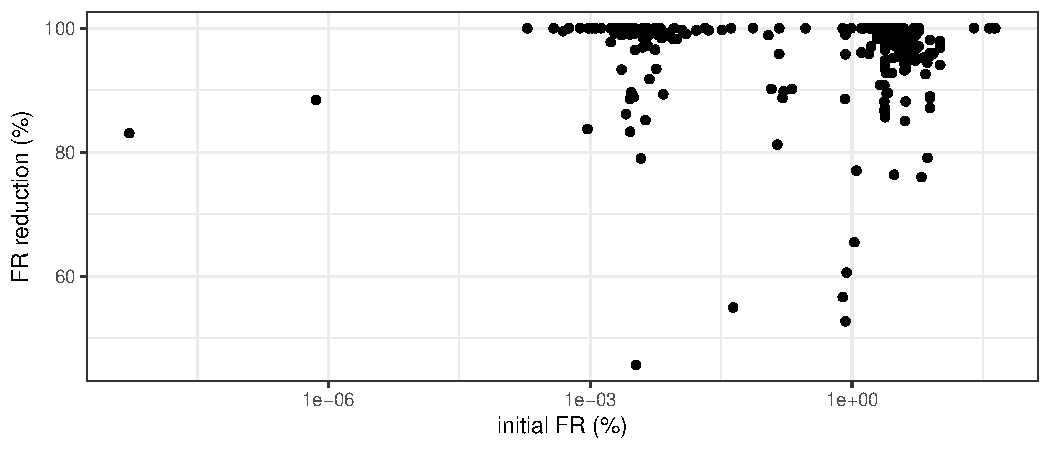
\includegraphics[width=.8\textwidth]{frRepairRed}
\caption{Relation between the initial fault ratio and the fault ratio reduction}
\label{fig:frRepair}
\end{figure*}
%
It seems that there is no proper correlation: we reduce (or do not reduce) the fault ratio in the same proportion among models having different initial fault ratios. We checked the correlation with the Spearman rank-order correlation coefficient~\cite{Wohlin2012}, and indeed we found a value of 0.23 indicating almost no correlation~\cite{hinkle2003applied}.

\researchquestion{Are the final models similar to those produced by SPL designers?}

The main aim of the proposed approach is to obtain a feature model that satisfies all the change requirements; to this purpose, we use the fault ratio as measure of model correctness. However, the final model we obtain, although correct, may be not readable by and not useful for an SPL designer. Although we could not ask real SPL designers to validate our models in terms of usefulness and readability, we have access to models developed by SPL designers to achieve the same update requests we tackled in the experiments (models $\fm_t$ used as target in the experiments). We can assume that SPL designers are likely to find our models useful if models produced by our process are similar to their models. We therefore measure the {\it readability} of the final model of our process in terms of {\it distance} from the model $\fm_t$ developed by a designer for the same update request. We compute the {\it edit distance}~\cite{pawlik_efficient_2015,pawlik_tree_2016} of the final model $\fm_f$ from $\fm_t$, defined as the number of {\it edits} (insertion, deletion, and rename of tree nodes) that we have to apply to $\fm_f$ in order to obtain $\fm_t$.\footnote{Note that these edit operations are more fine-grained than our mutation operators and we are always able to compute the distance between two feature models.} Table~\ref{tab:processPerformance} reports also the edit distance (ED) to the target model (average among the models), and the percentage of models that are syntactically equal and semantically equivalent to the target model. Of course, models not completely updated are not syntactically equal to the target and have edit distance greater than 0. Completely correct models (semantically equivalent) are often also syntactically equal (for example, 86.67\% of the {\tt PPU d1} models are semantically equivalent and 48.33\% are also syntactically equal); however, there are some correct final models that are different from the target model $\fm_t$ (for example, {\tt HelpSystem} is completely updated 86.67\% of the times, but always in a different way than $\fm_t$).


\researchquestion{Does considering the number of cross-tree constraints in the fitness impact the final results?}

As explained in Sect.~\ref{sec:prodBasedChangeReqs}, our fitness function (see Eq.~\ref{eq:fitness}) can also take into consideration the number of cross-tree constraints ($\mathit{ctc}$); the value we selected for $k$ (see Eq.~\ref{eq:kFitness}) has the aim of penalizing models with higher $\mathit{ctc}$ at the same fault ratio (in order to limit the insertion of such constraints and instead give precedence to changes of the parental relations). In order to assess the impact of this choice, we have executed the same experiments presented before with $k=0$ in the fitness function (that becomes $\fitness(\fmp) = 1 - \FR(\fmp, t)$) and $\thT=1$. Table~\ref{tab:performanceVsConstraints} reports the data in terms of average fault ratio reduction, percentage of semantically equivalent, percentage of syntactically equal models, and the average number of cross-tree constraints.
%
\begin{table}[!tb]
\caption{Performance of the updating process with the two versions of the fitness}
\resizebox{1\textwidth}{!}{%
\centering
\setlength\tabcolsep{2pt} 
\begin{tabular}{llrrrr|rrrr}
\toprule
& SPL & \multicolumn{4}{c}{Fitness without constr. ($k=0$)} & \multicolumn{4}{c}{Fitness with constr. ($k$ as in Eq.~\ref{eq:kFitness})}\\
\midrule
& & \shortstack{FR\\reduction (\%)} & \shortstack{sem.\\eq. (\%)} & \shortstack{synt.\\eq. (\%)} & ctc & \shortstack{FR\\reduction (\%)} & \shortstack{sem.\\eq. (\%)} & \shortstack{synt.\\eq. (\%)} & ctc \\
\midrule
\multirow{12}*{\rotatebox{90}{\small \benchReal}} & {\tt MobileMedia d1} & 94.10 &  61.11 & 17.78 & 0.69 &  96.03 &  64.44 & 17.78 & 0.23 \\
& {\tt MobileMedia d2} & 84.83 &   0.00 &  0.00 & 1.85 &  86.54 &   0.00 &  0.00 & 0.63 \\ 
& {\tt MobileMedia d3} & 85.16 &   0.00 &  0.00 & 2.43 &  86.13 &   0.00 &  0.00 & 0.80 \\ 
& {\tt HelpSystem} & 97.22 &  86.67 &  0.00 & 5.57 &  96.92 &  86.67 &  0.00 & 5.57 \\ 
& {\tt SmartHome} &   88.42 &   0.00 &  0.00 & 0.53 &  88.42 &   0.00 &  0.00 & 0.43 \\ 
& {\tt ERP\_SPL} &   82.96 &   0.00 &  0.00 & 0.40 &  83.08 &   0.00 &  0.00 & 0.43 \\ 
& {\tt PPU d1} & 98.10 &  87.50 & 45.83 & 1.62 &  97.44 &  86.67 & 48.33 & 1.23 \\ 
& {\tt PPU d2} & 95.89 &  68.57 & 37.14 & 2.11 &  96.48 &  68.57 & 36.67 & 1.39 \\ 
& {\tt PPU d3} & 87.25 &  50.00 & 27.22 & 2.95 &  87.43 &  48.89 & 28.89 & 1.94 \\ 
& {\tt CAR d1}  & 73.61 &  55.56 &  3.33 & 1.89 &  69.81 &  57.78 &  6.67 & 0.77 \\ 
& {\tt CAR d2}  & 78.06 &  45.00 &  0.00 & 3.22 &  80.31 &  50.00 &  0.00 & 1.83 \\ 
& {\tt CAR d3}  & 62.80 &   0.00 &  0.00 & 4.63 &  65.52 &   0.00 &  0.00 & 2.37 \\ 
\midrule
\multirow{4}*{\rotatebox{90}{\small \benchMut}} & {\tt Register} &   96.11 &  82.70 & 64.03 & 0.60 &  95.84 &  80.27 & 65.20 & 0.22 \\ 
& {\tt Graph} & 100.00 & 100.00 & 99.37 & 0.00 & 100.00 & 100.00 & 99.03 & 0.00 \\ 
& {\tt Aircraft} &  97.43 &  85.97 & 68.73 & 0.42 &  97.49 &  84.53 & 68.63 & 0.29 \\ 
& {\tt Connector} & 98.05 &  93.70 & 63.00 & 0.48 &  98.11 &  94.00 & 68.47 & 0.20 \\ 
\bottomrule
\end{tabular}%
}
\label{tab:performanceVsConstraints}
\end{table}
%
For easing the comparison, we also report the same data of the results obtained with the previous experiment (already reported in Table~\ref{tab:processPerformance}). In order to check whether the consideration of cross-tree constraints has some effect on the final results, we have applied to the data the classical hypothesis testing by performing the Wilcoxon signed-rank test\footnote{We performed a non-parametric test as we found, with the Shapiro-Wilk test, that the distributions are not normal.}~\cite{Wohlin2012} between the results with the two versions of fitness. The null hypothesis that considering $\mathit{ctc}$ has no impact of the final model cannot be rejected for the percentage of totally updated models (i.e., semantically equivalent), but it is rejected for the syntactical equivalence with $p$-value equal to 0.0038. This confirms that penalizing  the usage of cross-tree constraints in the fitness improves the quality (readability) of the final model without compromising the ability of the approach in achieving the update request.


\section{Threats to validity}\label{sec:threats}
We discuss the threats to the validity of our results along two dimensions, \emph{external} and \emph{internal} validity~\cite{Wohlin2012}.

\subsection{External validity}\label{sec:externalValidity}

Regarding external validity, a threat is that the obtained results could be not generalizable to real-world (industrial) feature models having specific update requests. However, as first benchmark, we have selected 9 couples of models showing the evolution of real SPLs~\cite{multimediaPaper,helpSystemPaper,smartHomePaper} taken from the SPLOT repository, and other 27 couples from the evolution of other two real SPLs described in literature~\cite{Burdek2016,Pleuss2012} (see Sect.~\ref{sec:benchmarks}); moreover, in order to enlarge the set of evaluated models, we generated 400 input models by randomly mutating other 4 feature models (acting as target). We believe that this way of selecting the benchmarks reduces the bias w.r.t. other real models this process may be applied to in the future.

Another threat to the external validity could be that the proposed process does not scale well to models larger than those considered in the experiments. In particular, the time for computing the fitness function grows exponentially with the number of features, as it is based on BDD construction. In order to address this problem, as future work, we plan to devise a technique that, given a single change requirement $c$, identifies the sub-tree $\mathit{st}$ of the feature model {\it affected} by $c$, i.e., $c$ can be achieved by only modifying $\mathit{st}$; only considering $\mathit{st}$ would allow to improve the process performance, as the mutations would be more targeted and the fitness computation would be performed on a smaller BDD.

Another threat to the external validity is that the update requests that we use in the experiments could be different by those written by SPL designers. However, update requests have been obtained by computing the difference of consecutive versions of feature models written by SPL designers. While change requirements \Ftbr, \Fadd, and \Frem are guaranteed to be the same as those specified by SPL designers, \CFrelax and \CFrem are only semantically equivalent. However, this is not a threat, as the evolutionary approach only considers the semantics of the \CFrelax and \CFrem, not their structure.

\subsection{Internal validity}\label{sec:internalValidity}

Regarding internal validity, a threat is that the obtained results could depend on the values chosen for the parameters of the evolutionary process (parameters of termination conditions, and parameters of the selection and evolution phases) and that, with some other values, the results would have been different (e.g., a given selection strategy could perform better); although we kept all the parameters fixed, we believe that the overall result that our approach is able to actually update the feature model is not affected. However, as future work, we plan to perform a wider set of experiments in which the effect of each single parameter is evaluated. For finding the best parameter setting, we could use a parameter-tuning framework as irace~\cite{irace}.
\end{tikzborder}




\part{Test-Driven Model Repair}
\chapter{Repair of Configuration Constraints}
A model for a combinatorial problem consists of parameters which can take various domain values. Combinatorial models may have also constraints among parameter values to, for example, model inconsistencies between certain hardware components, limitations of the possible system configurations, or simply because of design choices \cite{gargantini_combinatorial_2017}.
%Some methods have been introduced to automate the process of inferring constraints, but they do not aim at \textit{repairing} existing ones \cite{abukwaik_extracting_2016,Temple:2016:UML:2934466.2934472}. 
%Therefore, in \cite{gargantini_combinatorial_2017}
The devised iterative approach uses a fault-localization tool based on combinatorial testing, called BEN \cite{ghandehari2018combinatorial}, and CIT policies introduced in \cite{Gargantini16:validation} to find failure-inducing combinations of parameter values.
The model is then repaired \textit{logically}, by translating such failure-inducing combinations into expressions in propositional logic.
The repairs are of two types, depending on whether the model is true and the system (i.e., the oracle) false for a given test case (in this case, the model is \textit{under-constrained}) or vice-versa (in this case, the model is \textit{over-constrained}). Tab. \ref{table:testsandfaults} reports possible scenarios in which such condition may occur in a system with three boolean parameters A, B, C, that map to directives in a C program in which both B and C can be enabled only if also A is activated.
\begin{table}[!hb]
	\caption{Test suites with faults (in gray)}\label{table:testsandfaults}
	\centering
	\resizebox{.8\columnwidth}{!}{
		\begin{subtable}[t]{.5\columnwidth}
			\centering
			\caption{\underConstr fault}
			\label{table:underConstrFault}
			\begin{tabular}{c|c|c||c|c}
				A & B & C & \mfU & oracle\\
				\hline 
				T & T & F & \cg T & \cg F\\% & \underConstr fault\\
				T & F & F & F & F\\
			\end{tabular}
		\end{subtable}%
		\begin{subtable}[t]{.5\columnwidth}
			\centering
			\caption{\overConstr fault}
			\label{table:overConstrFault}
			\begin{tabular}{c|c|c||c|c}
				A & B & C & \mfO & oracle\\
				\hline 
				F & T & T & T & T\\
				F & F & T & T & T\\
				F & T & F & \cg F & \cg T\\% & \overConstr fault\\
				F & F & F & \cg F & \cg T\\% & \overConstr fault\\
			\end{tabular}
		\end{subtable}%
	}
\end{table}


Experiments for five real-world systems (Libssh, Telecom, Aircraft, Concurrency, and Django) show that our approach can repair on average 37\% of conformance faults. Moreover, we also notice that it can infer and repair parameter constraints for the configurations that lead to a successful startup of Django, a well-known open source web application framework written in Python.

%For test generation we used a framework called CTWedge

%\subsubsection{XSS Vulnerabilities Constraints}
%Combinatorial models are also suitable to model parts of XSS attack vectors, with a limited number of possible values.
%We applied our iterative approach also to such models, using as oracle a script that runs the web application under test, inject the attack vector in a particular input field in a form, and checks wether the injected Javascript code has been present in the response page.  We evaluated our approach empirically on four systems from the Web Application Vulnerability Scanner Evaluation Project (WAVSEP), and on two real-world web applications, obtaining an accurate model of the constraints among parameters that cause an attack vector to break the sanitization function of the system.

\section{Using Iterative Constraint Repair to Detect XSS Vulnerabilities}
\chapter{Repairing Timed Automata Clock Guards through Abstraction and Testing}

\part{Tools to Support Model Repair}
\chapter{CTWedge: Migrating Combinatorial Interaction Test Modeling and Generation to the Web}
\begin{tikzborder}{\cite{IWCTGargantini2018}}
	Combinatorial Interaction Testing (CIT) is becoming a widespread practice for software testing.
The presence of tools for CIT is of fundamental importance because performing CIT activities manually can be error prone and time consuming. The site pairwise.org\footnote{See \url{http://www.pairwise.org/tools.asp}} lists at least 43 tools supporting several CIT activities while the paper~\cite{Nie2011} reviewed the CIT literature and found around 20 tools. 
%
%\begin{mdframed}
Most of the tools are classical programs or plugins of existing programs/platforms.  In all these cases, the user has to download, install, and execute the program on his/her machine.  Some tools offer a GUI interface, for example, for defining the models and run the test generation, while others rely on other programs for some activities (like PICTMaster, based on PICT~\cite{czerwonka_pairwise_2006}, that works entirely inside Microsoft Excel). %(like PICT~\cite{czerwonka_pairwise_2006} that gives the output as an Excel spreadsheet).
In~\cite{citlab12} we have presented a plugin for the eclipse IDE that helps the user in writing CIT models with constraints by leveraging all the expected features of a modern IDE, and it generates combinatorial test suites by using third party programs (like CASA or ACTS).
%\end{mdframed}
However, this classical approach poses some challenges. First, the user must install the chosen CIT tool, which in turn may require some dependencies, like java, or in case of plugin, it requires the installation of another program or application like eclipse, excel and so on. Then the user must use his/her machine for running the test generation algorithms. For experienced users with powerful machines they can administer, this is not a real problem. However, for novice users with not so powerful computer, or students that are just learning the CIT principles, or software developers using computer they cannot administer, this can become a cost to be considered and it may be an obstacle for the use of CIT.

Second, from the point of view of tool developers, the distribution of programs means that they have little or no control on the software once is installed: when a bug is discovered the developer has to fix the bug, publish a new version of the tool and hope that the users will update their software. Moreover, the developer has no idea about how the software is used: what are the typical scenarios of use (big or small models, for example), what are the features that are mostly used (for example, what modeling features are more used). Furthermore, it is difficult for tool developers to apply a cost model able to reward their effort in developing and deploying the CIT tool. Indeed, most of the tools are given away for free by researchers supported by their own organization.

A possible solution of these problems could be the offer of CIT features as software as a service (SaaS). SaaS is software that is accessed t+hrough Internet by using a classical web browser.  The SaaS software is actually hosted on the vendor’s servers, and the customers log in and perform tasks as necessary.  The 
vendor is the one who is ultimately responsible for hosting, upgrading and maintaining the program as needed.  There is an extensive literature about SaaS and the advantages (together with limitations) are well known~\cite{Menken:2008}. 

There are already experiences in using the web for CIT. For instance, CTWeb Classic~\cite{usaolaframework}, CTWeb Plus~\cite{ctwebplus}, TestCover~\cite{testcover}, Hexawise~\cite{hexawise}, and PairWiser~\cite{pairwiser}. 

However, as we will discuss in the related work section, each tool has its own specific language to define combinatorial models, with its own predefined output formats and a (limited) set of supported existing or in-house algorithms for test case generation. Not all those tools are equally powerful or easy to use, and many of them are commercial or require registration.

%However, as we will discuss in the related work section, they lack of some features: very limited editing capabilities, little support for constraints, test generation using in-house algorithms, and limited export formats.

For this reason, starting from our experience with \citlab~\cite{citlab12}, we have worked on a web based application that allows the user to write CIT models in a similar way he/she would do in a classical IDE and it offers test suite generation by means of   server using known and community evaluated test generation algorithms. 
Our system, called \ctwedge (Combinatorial Testing Web EDiting and GEneration), introduces a rich language for combinatorial models, offers a powerful web editor, and allows the user to generate the CIT test suites on a server. The only software needed to use \ctwedge is a modern web browser.

The paper is organized as follows. In Sect. \ref{sec:language} we present the modeling language (in an abstract way) we use to define CIT models. In Sect. \ref{sec:ctwedge} we introduce our tool, its architecture, its web editing capabilities, and the generator engine. A detailed comparison with other similar web based tools is presented in  Sect. \ref{sec:related}. Future works and possible directions of extension are presented in Sect. \ref{sec:futurework}. Sect. \ref{sec:conclusions} concludes the paper.


\section{A simple language for CIT models}\label{sec:language}

We have devised a simple textual language for CIT models which is suitable to be used in web editors. It allows the definition of parameters, each with its name and (finite) domain, and it is based on our previous language defined for \citlab \cite{citlab12}. We allow the following parameter types: 

\begin{enumerate}
	\item \textsf{Boolean} with only two possible values \textsf{true} and \textsf{false} (all lower or all upper case).
	The two boolean constants are also considered of Boolean type.
	\item \textsf{Ranges} that are integer intervals defined by their lower bound $l$ and upper bound $u$. With $[l..u]$ we denote all the integers between $l$ and $u$ included.
	\item \textsf{Enumerative} that are a list of possible values between \{\}. We are rather liberal about the elements and we allow identifier starting also with a number, natural numbers, and strings. For example, one could define a  enumerative \textsf{values} in this way:
	\begin{lstlisting}[language=ctwedge]
	values : {100, 1M, "my name", cit}
	\end{lstlisting}
\end{enumerate}

A simple example of combinatorial model with three parameters is shown in Fig. \ref{fig:ctexample}. 

\begin{figure}[tb]
	\centering
	\begin{lstlisting}[language=ctwedge,frame= single]
	Model Phone
	Parameters:
	emailViewer : Boolean
	textLines:  [ 25 .. 30 ]
	display : {16MC, 8MC, BW}
	\end{lstlisting}
	\caption{A smartphone example}
	\label{fig:ctexample}
\end{figure}

There are some semantic rules about the parameters and their definitions, defined as follows:
\begin{enumerate}
	\item The name of each parameter must be unique.
	\item In \textsf{Ranges}, the lower bound $l$ must be less than the upper bound $u$.
	\item The elements in each \textsf{Enumerative} must be distinct. We allow two enumerative parameters to share some elements, though.
\end{enumerate}


\subsection{Constraints}

A distinctive feature of our language is the support of modeling constraints among parameters. 
In most configurable systems, constraints or dependencies exist between parameters. 
Constraints may be introduced for several reasons, for example, to model inconsistencies between certain hardware components, limitations of the possible system configurations, or simply design choices~\cite{CohenISSTA07}.
In our approach, tests that do not satisfy the constraints are considered \emph{invalid} and do not need to
be produced. 
For this reason, the presence of constraints may reduce the number of tests of the final test suite (but it may also increase it ~\cite{CohenISSTA07}).
However, the generation of tests considering constraints is generally more challenging than the generation without them, and several test generation techniques still do not support constraints, at least not in a direct manner.
In \ctwedge we decided to focus more on techniques supporting constraints.

In \ctwedge, we adopt the language of propositional logic (with the usual logical operators) with equality and arithmetic to express constraints. 
To be more precise, we use propositional calculus, enriched by the arithmetic over the integers and enumerative symbols. As operators, we admit the use of equality and inequality for any variable, the usual Boolean operators for Boolean terms, and the relational and arithmetic operators for numeric terms. 
To be more precise, Table \ref{tab:validity} reports all the rules we have defined to check if a constraint is semantically correct.

\begin{table*}
	\centering
	\resizebox{\textwidth}{!}{
	\begin{tabular}{|l|l|l|}
		\hline 
		\textbf{Expression}	& \textbf{Case} & \textbf{Correct iff}\\\hline
		\multirow{7}{*}{\shortstack{$e_1\ op\ e_2$	with $op \in \{=, \neq \}$ $\rightarrow boolean$ \\ $ e_2\ op\ e_1$ with $op \in \{=, \neq \}$ $ \rightarrow boolean$ }}  & $e_1$ enumerative, $e_2$ element& $e_2$ belongs to $e_1$ elements \\\cline{2-3}
		
		& $e_1$ enumerative, $e_2$  enumerative& $e_1$ and $e_2$ share at least one element \\\cline{2-3} 
		&  $e_1$ range, $e_2$ range & $e_1$ and $e_2$ share at least one number \\\cline{2-3}
		& $e_1$ range, $e_2$ number & always \\\cline{2-3}
		& $e_1$ number, $e_2$ number & always \\\cline{2-3}
		& $e_1$ boolean, $e_2$ boolean & always\\\cline{2-3}
		\hline 
		
		\multirow{3}{*}{\shortstack{$e_1\ op\ e_2$	with $op \in \{<, \le, >, \ge \}$ $\rightarrow boolean$ \\ $ e_2\ op\ e_1$ with $op \in \{<, \le, >, \ge \}$ $ \rightarrow boolean$ }}  &  $e_1$ range, $e_2$ range & $e_1$ and $e_2$ share at least one number \\\cline{2-3}
		& $e_1$ range, $e_2$ number & always \\\cline{2-3}
		& $e_1$ number, $e_2$ number & always \\\cline{2-3}
		\hline 
		
		\multirow{3}{*}{\shortstack{$e_1\ op\ e_2$	with $op \in \{\wedge, \vee, \rightarrow\}$ $\rightarrow boolean$ \\ $ e_2\ op\ e_1$ with $op \in \{ \wedge, \vee, \rightarrow \}$ $ \rightarrow boolean$ }}  & \multirow{3}{*}{$e_1$ boolean, $e_2$ boolean} & \multirow{3}{*}{always} \\ %\cline{2-3}
		& & \\
		& & \\ 
		\hline
				
		\multirow{1}{*}{$\neg e$ $ \rightarrow boolean$}  & $e$ boolean & always \\\cline{2-3}
		\hline
		
		\multirow{4}{*}{$e_1\ op\ e_2$	with $op \in \{+, -, *, /, \%\}$ $\rightarrow number$}  & $e_1$ number, $e_2$ number & $e_2 \neq 0$ if $op=/$ or $op=\%$ \\\cline{2-3}
		& $e_1$ range, $e_2$  range & always \\\cline{2-3} 
		&  $e_1$ range, $e_2$ number & $e_2 \neq 0$ if $op=/$ or $op=\%$ \\\cline{2-3}
		&  $e_1$ number, $e_2$ range & always \\\cline{2-3}
		\hline
	\end{tabular} 
}
	\caption{Rules of \ctwedge Language Validator for Constraints}\label{tab:validity}
\end{table*}

For example, we can write constraints in this way:

\begin{lstlisting}[language=ctwedge,frame= single]
Model Phone
..
Constraints:
# emailViewer => textLines > 28 #
# emailViewer and display != 16MC => textLines > 28 + 3#
\end{lstlisting}

Many test suite generation tools provide a limited support for constraints. For instance, AETG \cite{Cohen_1997,Lott:2005:MRC:1083274.1083281} allows only simple constraints of type \textsf{if then else} or \textsf{requires}. The language of \ctwedge is in this aspect more expressive, as it is targeted to be more general than existing tools. In the specific case of AETG, the translation of those templates into our logic is straightforward. For example the \textsf{if then else} constraint can be translated by two implications.
Other tools \cite{CohenISSTA07} allow constraints only in the form of forbidden combinations \cite{Golumbic:2011:GTC:2028636}. Our language is more general, as a forbidden tuple would be translated as a \textit{not} statement. For instance, a forbidden pair \textsf{emailViewer = false; display = 16MC} would be represented by the following constraint:
$$\textsf{\#\ not\ (emailViewer = false\ and\ display = 16MC)\ \#}$$
However, the explicit list of the forbidden combinations may explode and it may become impractical and error-prone to represent it. For example, if the model of mobile phones presented in Fig. 1 had a constraint that

\emph{"A front video camera requires also a 16MC display"}. This constraint would be translated into two forbidden tuples:

$$\textsf{(emailViewer = true, display = 8MC);}$$
$$\textsf{(emailViewer = true, display = BW);}$$
However, the translation as constraint in general form would be simply:
$$\textsf{\#\ emailViewer =\textgreater\ display = 16MC\ \#}$$
which is more compact and more similar to the informal requirement.

In our language semantics, a test case is valid only if it does not contradict any constraint in the specification. Others \cite{BRYCE2006960} distinguish between combinations to be avoided \textit{if possible} (soft constraints), and the forbidden combinations (hard constraints), which must always be avoided (our case). %We consider only hard constraints, for now.

Other tools, like CASA \cite{CASAwebsite}, support only constraints in conjunctive normal form, without arithmetic or relational operators.


\subsection{Xtext}

There are countless ways to define a language together with its parser. One emerging technique for Domain Specific Language modeling is the use of Xtext~\cite{Eysholdt:2010}. By defining the grammar of the DSL of choice by means of a Xtext grammar, the language designer obtains a parser, APIs to programmatically access models, a serializer and a smart editor for it. The editor provides many features out-of-the-box, such as syntax highlighting, content-assist, folding, jump-to-declaration and reverse-reference lookup across multiple files.  We had already used Xtext for defining the language in \citlab~\cite{citlab12}. Xtext support also the generation of a web editor, as we present in the following section.

Grammar rules written in Xtext are very close to the standard (E)BNF production rules. For instance, the main grammar rule that defines the whole CIT model is defined as follows:

\begin{lstlisting}[language=Matlab,columns=fullflexible,basicstyle=\small\ttfamily,stringstyle=\ttfamily\color{blue},upquote=true]  
CitModel:
'Model' name=ID 
'Parameters' ':' (parameters+=Parameter)+ 
('Constraints' ':' (constraints+=Constraint)+)?
\end{lstlisting}

Xtext can display the production rules by means of syntax diagrams, also known as railroad diagrams. For example, the rule presented before for {\small\ttfamily CitModel} is shown in Fig. \ref{fig:grammarrule}.

\begin{figure}
	\centering
	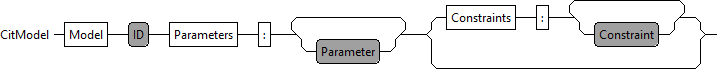
\includegraphics[width=1\linewidth]{images/grammar_rule}
	\caption{{\small\ttfamily CitModel} rule diagram}
	\label{fig:grammarrule}
\end{figure}

Because Xtext is based on ANTLR, it does not allow left recursive parser rules and parsing nested expressions is not as simple as writing a EBNF rule. The \ctwedge language parses the constraints by defining the precedence among operators implicitly by left-factoring expression definitions. For example, in order to parse the AND operators before the OR operators,  \ctwedge  introduces the following two rules that are not left recursive:

\begin{lstlisting}[language=Matlab,columns=fullflexible,basicstyle=\small\ttfamily,stringstyle=\ttfamily\color{blue},upquote=true,morekeywords={returns}]  
OrExpression returns Expression:
AndExpression ({OrExpression.left=current} 
OR_OPERATOR (right=AndExpression))*;

AndExpression returns Expression:
EqualExpression ({AndExpression.left=current}
AND_OPERATOR (right=EqualExpression))*;
\end{lstlisting}



The definitions of semantic constraints in Xtext is performed by user-defined validator classes written in Java or in Xtend containing methods annotated by {\small\ttfamily @Check}. For instance, to check that in the definition of any range domain of our CIT models  the upper bound is greater than the lower bound, we have introduced the following checking method:

\begin{lstlisting}[language=Java,morekeywords={def},basicstyle=\small\ttfamily]
@Check
def checkRangeIsCorrect(Range range) {
if (range.getBegin() >= range.getEnd())
error("The second term must be greater ...");
}
\end{lstlisting}

\section{\ctwedge: CT Web Editor and Generator}\label{sec:ctwedge}

In this section, we present our tool \ctwedge. 
As we can see in Fig.~\ref{fig:architecture}, the tool is composed by a language definition component (with its Xtext parser and validator), a web-based editor for the \ctwedge language, with some options for test generation and a test suite visualizer and exporter, and a test suite generator that exploits third-party test generation tools.

The tool is written in Java and Xtext, and can be deployed on any Web-application server, such as Apache Tomcat. It is publicly available at: \url{http://foselab.unibg.it/ctwedge/}.


\begin{figure}[bt!]
	\centering
	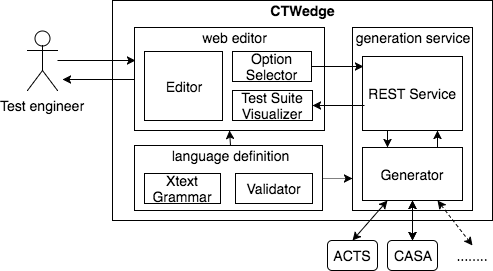
\includegraphics[width=\columnwidth]{images/architecture.png}
	\caption{\ctwedge architecture}\label{fig:architecture}
\end{figure}


\subsection{Combinatorial Testing Web Editor}

In order to implement a web-based editor, we can leverage the Xtext framework, since Xtext starting from version 2.9 offers an interface for integration of text editors in web applications. The text editors are implemented in JavaScript, and language-related services such as code completion are realized through HTTP requests to a server-side component.

The Xtext web-based editor provides several features, like content assist to help the user to complete the models, validation to check the correctness, syntax coloring, and formatting.

The \ctwedge web editor is based on Ace (Ajax.org Cloud9 Editor)\footnote{See \url{https://ace.c9.io/}}, but other web editors (like Orion and CodeMirror) are available. Xtext does not yet provide support for the recently standardized Language Server Protocol \cite{lsp}, which we plan to include in our tool as a future work.  A screenshot of the \ctwedge web editor is shown in Fig. \ref{fig:editor}. The web editor provides an immediate feedback while writing by means of syntax highlighting, auto completion, and errors markings. 

The validation of the model is performed run-time while the user writes it. If the validator finds an error in the model, it generates an error message. The nature of the error is indicated in the pop-up box appearing when positioning the cursor over the error sign, and the point in which the error occurs is marked in the editor. Fig. \ref{fig:validation} shows how model validation errors are displayed to the test engineer.

\begin{figure*}[bt!]
	\centering
	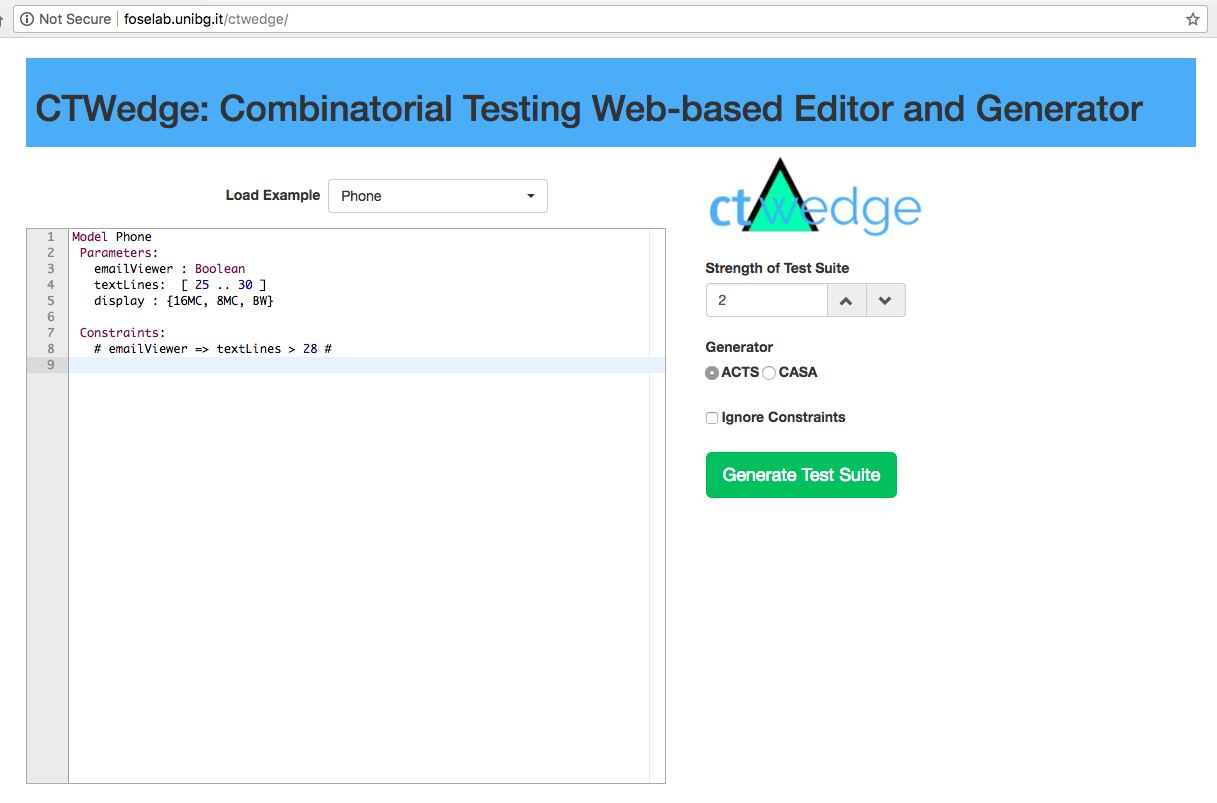
\includegraphics[width=\textwidth,trim={0 10cm 0 0},clip]{images/editor2.png}
	\caption{\ctwedge web editor}\label{fig:editor}
\end{figure*}

The editor allows to load predefined examples of combinatorial models, selected from literature \cite{Segall2011} and converted into \ctwedge language format (with extension \textit{.ctw}).

\red{Graphical components (buttons and option selectors) are built using the JavaScript frameworks JQuery}\footnote{JQuery: \url{https://jquery.com/}} 
and Bootstrap\footnote{Bootstrap: \url{https://getbootstrap.com/}}.
\red{ The web application is fully compatible also with mobile devices (Android and iOS), from any recent Web browser with JavaScript enabled.}

\begin{figure}[bt!]
	\begin{subfigure}{\columnwidth}
		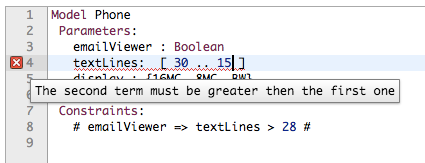
\includegraphics[width=.8\columnwidth]{images/validation1.png}\caption{Validation of Range parameter}
	\end{subfigure}
	
	\begin{subfigure}{\columnwidth}
		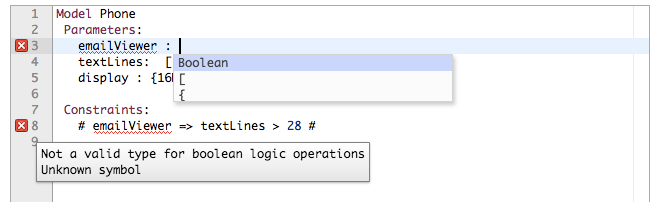
\includegraphics[width=\columnwidth]{images/validation2.png}\caption{Code recommender. Unknown symbol error.}
	\end{subfigure}
	
	\begin{subfigure}{\columnwidth}
		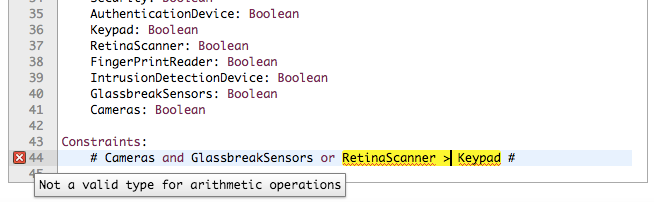
\includegraphics[width=1\columnwidth]{images/validation3.png}\caption{Validation of relational operations}
	\end{subfigure}
	\caption{Examples of \ctwedge validation errors}\label{fig:validation}
\end{figure}

\subsection{Test generator web service}

The function of actually generating a test suite from the test model and option parameter is web-served and performed by the test generation service which is the component of \ctwedge.
The test generation service is composed by two modules: a REST\footnote{REST: Representational State Transfer} service and a language translator.

The REST service handles input model and option parameters for the generation, calls the generators from which it gets back the tests and it is responsible to deliver them to the web browser. 

The test generator acts as a \textit{driver} between \ctwedge and the various third party combinatorial test generation tools, which are usually accessible via their own APIs, or via command line. The test generator exports the combinatorial model along with the generator options, into the the specific language of the external tool, or directly into the tool's APIs. Then, it waits for the generator to compute the test suite, and once ready, it passes it back to the REST service. If necessary, the generator also maps any parameter values back to the original \ctwedge model format. Each external program needs its own translator.

\begin{table}[!tb]
	\caption{Request parameters to \ctwedge generation service}
	\centering
	\resizebox{0.5\textwidth}{!}{%
		\centering
		\begin{tabular}{l l p{2.55cm} p{3.35cm}}
			\toprule
			\textbf{Parameter} & \textbf{type} & \textbf{description} & \textbf{values} \\
			\midrule
			model & String & the combinatorial model & as written and validated by the editor (see Sec. \ref{sec:language}) \\ 
			strength & Int & the combinatorial interaction strength & any integer above 1 (default is 2: pairwise) \\ 
			generator & Enum & the tool to be used & ["acts", "casa"] (so far) \\
			ignConstr & Boolean & if constraints should be ignored in test generation & ["true", "false"] (default is false) \\ 
			\bottomrule
		\end{tabular}
	}
	\label{tab:parameters}
\end{table}

The REST service accepts an HTTP GET or POST request with parameters as described in Tab. \ref{tab:parameters}.
For sake of brevity, an example URL request to the web generator service is shown in Fig. \ref{fig:urlexample}.

\begin{figure}[tb!] % https://tex.stackexchange.com/questions/116534/lstlisting-line-wrapping
	\centering
	\lstset{
		basicstyle=\ttfamily\small,
		columns=fullflexible,
		frame=single,
		breaklines=true,
		postbreak=\mbox{\textcolor{red}{$\hookrightarrow$}\space},
		language=url
	}
	\begin{lstlisting}
	http://foselab.unibg.it/ctwedge.generator?model=Model%20Phone%20Parameter:%20...>28%20#&strength=2&generator=acts&ignConstr=false	
	\end{lstlisting}
	\caption{Generator URL example}
	\label{fig:urlexample}
\end{figure}

So far, we interfaced \ctwedge with ACTS~\cite{ACTS} and CASA~\cite{CASAwebsite}. ACTS is accessed  via it internal APIs whereas CASA is called via command line.

The resulting test suite is returned in CSV\footnote{CSV: Comma Separated Values} format. The header line contains the parameter names, and each following line represents a single test, with parameter values.
The web front-end allows to download CSV file to further local use, and shows the test suite in the browser by converting it into an HTML table. Conversion is straightforward and done client-side via Javascript.

Arithmetic operations and relational operators ($>$, $<$, $\le$, $\ge$) are not natively supported by CASA, and in presence of such constraints, an error is reported to the user, as in Fig. \ref{fig:casaError}.

\begin{figure}[hbt!]
	\centering
	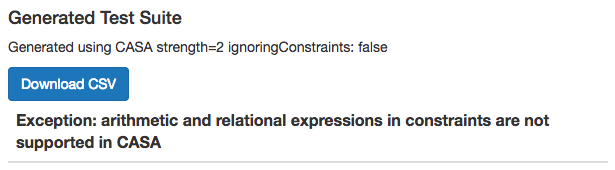
\includegraphics[width=\columnwidth]{images/casaError.png}
	\caption{Message of operations not supported in constraints for CASA generator tool}\label{fig:casaError}
\end{figure}

\begin{figure}[hbt!]
	\centering
	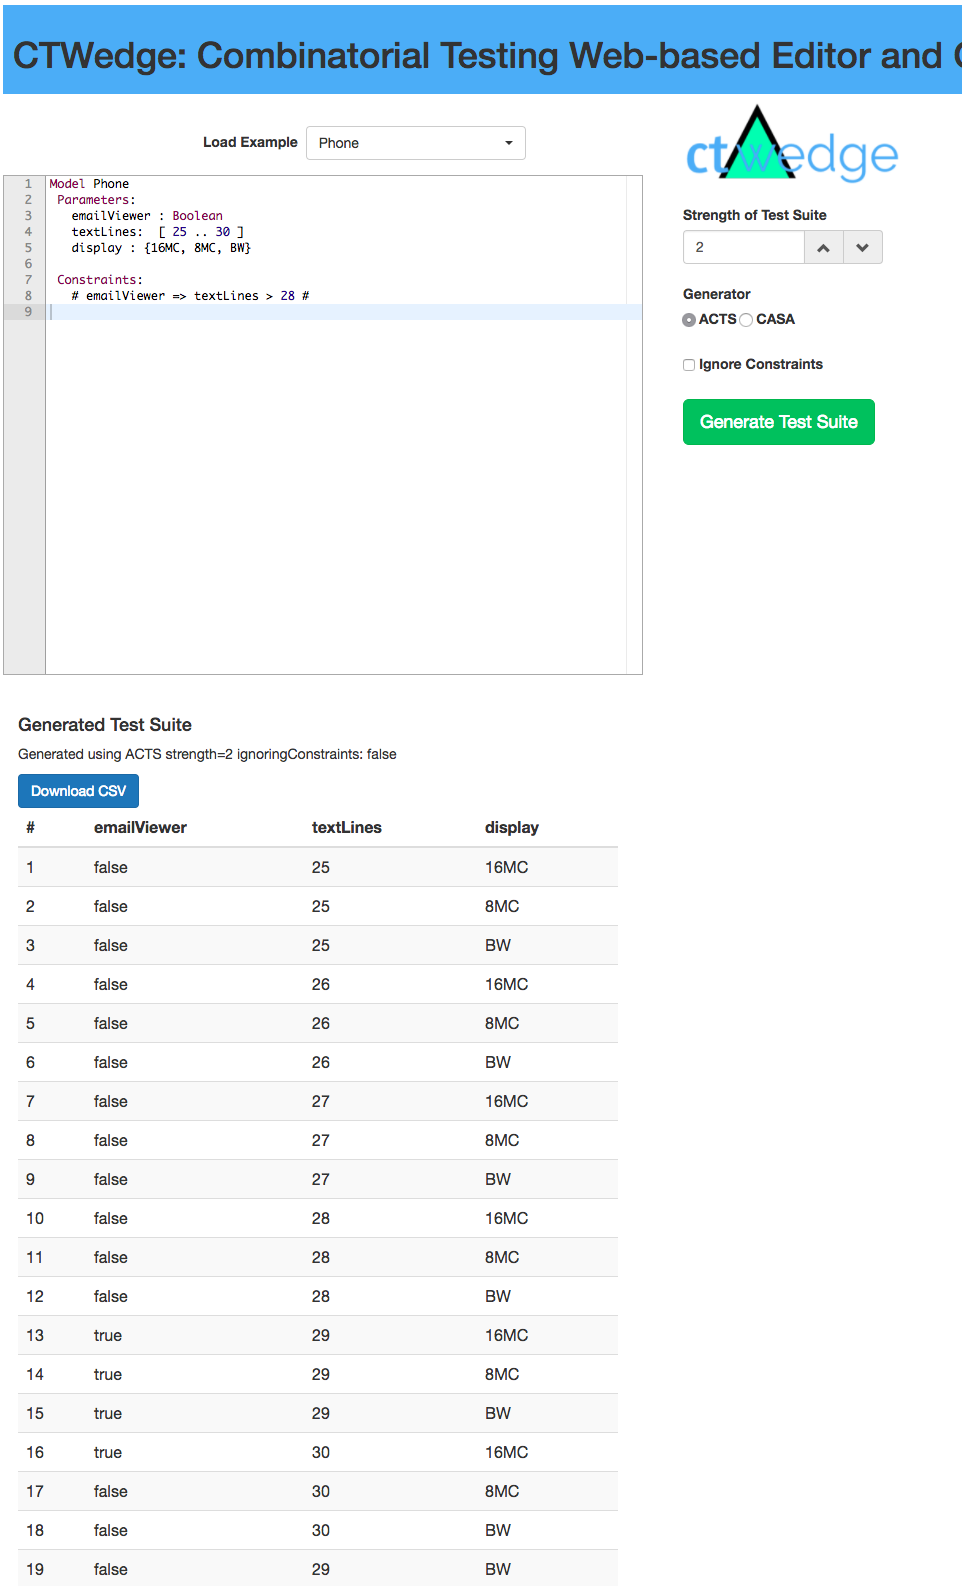
\includegraphics[width=.5\columnwidth,trim={0 0 7cm 0},clip]{images/generatedTable.png}
	\caption{\ctwedge visualization of the generated test suite}\label{fig:generated}
\end{figure}

The HTML table showing the generated test cases is located below the editor on the same window. This location is less invasive than a brand new tab as it does not hide or replace the current combinatorial model in the editor. Despite it is not immediately visible to the user, who may think the output is hidden, we believe that it preserving the access to the current screen is the most important aspect to be preserved.

The generator is called by the editor by AJAX, with an asynchronous XmlHttpRequest.


A screenshot of how the generated test suite is presented to the user is shown in Fig. \ref{fig:generated}. 
It is shown as plain HTML table, with the possibility to download the data as CSV. 

\section{Related Work}\label{sec:related}

With the success of the SaaS pattern, web-based tools have rapidly gained popularity due to their portability and ease of use. There exist some web-based services also for combinatorial test case generation, each with its own peculiarities. SaaS tools, however, still represents a small number of all the available tools for test case generation: IDE plugins and desktop applications represent almost the totality of the current tools. We looked for tools from the pairwise.org\footnote{See \url{http://www.pairwise.org/tools.asp}} and softwaretesters.net\footnote{See \url{https://softwaretesters.net/zbxe/index.php?mid=downloadtool&category=4258006&sort_index=readed_count&order_type=desc}} tool catalogs, and from the web, to the best of our searching skills. 


\begin{table}[bt!]
	\centering
	\footnotesize
	\setlength\tabcolsep{2pt}
	\begin{tabular}{l P{52mm} P{52mm}}
		Tool & URL & Documentation \\
		\toprule
		TestCover & \url{https://testcover.com} & \url{https://testcover.com/sub/instructions.php} (visible after registration) \\
		\midrule
		CTWebClassic & \url{http://alarcostest.esi.uclm.es/CombTestWeb/combinatorial.jsp} & \url{http://alarcostest.esi.uclm.es/CombTestWeb/stuff/usersManual.pdf} \\
		\midrule
		CTWebPlus & \url{http://www.testcasegeneration.com} or \url{http://www.ctwebplus.com/} & \url{http://www.ctwebplus.com/stuff/userManual.pdf} \\
		\midrule
		HexaWise & \url{https://hexawise.com/} & \url{https://hexawise.com/Hexawise_Introduction.pdf} \\
		\midrule
		PairWiser & \url{https://inductive.no/pairwiser/} & \url{https://inductive.no/pairwiser/knowledge-base/} \\
		\bottomrule
	\end{tabular}\caption{Tool resource links}\label{tab:docs}
\end{table}

We compare the following five SaaS for CIT, listed in Tab. \ref{tab:docs}:
\begin{itemize}
	\item TestCover~\cite{testcover} is a commercial web-based combinatorial test case generator supported by Testcover.com, LLC, founded in 2003. The tool was also presented at IWCT 2016~\cite{sherwood2016embedded}.
	\item CTWeb Classic~\cite{usaolaframework} is a free online tool for combinatorial testing and state machine test case generation,  developed at University of Castilla-La Mancha (Spain).
	\item CTWeb Plus~\cite{ctwebplus}, an academic combinatorial test generation tool developed as improvement of CTWeb Classic. CTWeb Plus is now commercially supported.
	\item HexaWise~\cite{hexawise}, a commercial combinatorial test case editor and generator, launched in 2009 by Hexawise, Inc.
	\item PairWiser~\cite{pairwiser}, a commercial web-based tool provided by Inductive AS. The online version was shut down January 15th, 2018. After that date, only the standalone application, for own-server installation, is available.
\end{itemize}

All tools are well documented, with examples and tutorials. Links of on-line editors and official documentation resources of these tools are shown in Tab. \ref{tab:docs}

\begin{table*}[hbt!]
	\resizebox{\textwidth}{!}{%
	\centering
	\setlength\tabcolsep{1pt}
	\tiny
	\begin{tabular}{p{1mm}lP{24mm}P{24mm}P{24mm}P{24mm}P{24mm}P{24mm}}
		%\hline
		& & \centering\textbf{TestCover}~\cite{testcover} & \centering\textbf{CTWeb Classic}~\cite{usaolaframework} & \centering\textbf{CTWeb Plus}~\cite{ctwebplus} & \centering\textbf{HexaWise}~\cite{hexawise} & \centering\textbf{PairWiser}~\cite{pairwiser} & {\textbf{\centering \ctwedge}} \\%\toprule
		\hline 
 
		\multicolumn{2}{l}{\textbf{Language}} & & & & & & \\ 	
		&	Parameter Definition & Enumerative & Enumerative & Enumerative & Enumerative, Ranges (via value expansion) & Enumerative & Boolean, Enumerative, Ranges \\%\midrule
		&	Constraints format & in DPB notation: via \emph{blocks} (i.e., sets of allowed combinations) & as \emph{if-then-else} & AND, OR, Else operators, not nested & invalid pairs (\emph{if..then..}) & guided by select boxes with rich choice of operators & arbitrary formula \\%\midrule
		
		&	Numeric operators & \cmark (in PHP functions) & \xmark & \cmark & \cmark & \xmark & \cmark \\%\midrule
		
		&	State Machine support & \cmark & \cmark & \cmark & \xmark & \xmark & \xmark \\\toprule 
		\textbf{Editing} & & & & & & \\
		&	Web-based editor & text area & text fields and buttons + file upload & text fields, buttons, drawing area & text fields and buttons & text fields and buttons & text area \\%\midrule
		&	Model Import/Export	& \cmark (Copy\&Paste as text) & \cmark & \xmark & \xmark & \xmark & \cmark   (Copy\&Paste as text)\\%\midrule	
		&	Helping facilities & \xmark & button-guided (no facilities to build input file to upload) & button-guided & button-guided & button-guided & content-assist, syntax highlight, in-line error reporting \\%\midrule 
		&	Example Models & \cmark & \cmark & to be rebuilt from documentation file, not one-click loadable & \cmark & in the documentation & \cmark \\\toprule
		
		\multicolumn{2}{l}{\textbf{Generation}} & & & &  & & \\%\midrule 
		&	n-wise & pairwise & pairwise & pairwise & up to 6-way interaction + mixed strength & up to 3-way interaction + mixed strength & \cmark \\%\midrule
		&	Supported generators & All-pairs & AETG, PROW, All combinations, Each choice, Random, Bacteriologic & AETG, Pairwise, All-combinations, Each-choice, Comb, Random & not specified & not specified & ACTS, CASA \\%\midrule
		&	Export formats & HTML, WSDL interface & HTML, CSV & HTML & HTML, Excel, CSV, OPML & Excel, Jira issues & CSV, HTML \\%\midrule
		&	Generate test scripts & \cmark (for Selenium) & \cmark (custom) & \cmark (custom) & \xmark & \cmark (custom) & \xmark \\%\midrule
		&	Coverage visualization & \cmark & \xmark & \xmark & \cmark & \cmark & \xmark \\\toprule 
		\multicolumn{2}{l}{\textbf{Other information}} & & & & & & \\%\midrule
		&	License & Commercial & Free & Commercial & Commercial & Commercial & Free \\%\midrule
		&	Registration & subscription required &  optional & subscription required & subscription required & own-server installation & \xmark \\%\midrule
		&	Online storage & \cmark & \xmark & \cmark & \cmark & \cmark (on own server) &\xmark  \\%\midrule
		&	Additional notes & Functions in PHP into constraints. Also accessible via WSDL interface.
		& Registration required for models with more than 5 parameters & Features a drawing area to represent states and transition of a state machine. The combinatorial model must be in the form of a state machine. & Has also a chart showing the interaction coverage after each test & Pairwiser online was shut down January 15, 2018. Available only for own-server installation. Allows to specify combinations to include in test suite. & -- \\\bottomrule 
	\end{tabular}
	}
	\caption{A comparison with other SaaS for CT}\label{tab:comparison}
\end{table*}

To compare the SaaS tools among them and w.r.t. \ctwedge, we consider the following aspects, that we believe to be among the most relevant for a test engineer interested in using a web-based combinatorial test generation tool:

\begin{itemize}
	\item \textbf{Language}. We look into the expressiveness of the accepted format for the combinatorial model in input. This evaluation includes:
	\begin{itemize}
		\item Parameter definition: how the parameter types and values  can be defined. For instance, a tool may support Boolean parameters or ranges of integers to express an enumerative made of all integers between two numbers.
		\item Constraint format: if the constraints can be expressed as free combinations of logical and arithmetic operations among parameters, or have special formats, such as a set of forbidden tuples, a set of implications, or a set of if-then-else conditions. 
		\item Numeric Operations: if constant numbers and basic numeric operations (+, -, *, /) are allowed in the constraints and/or in the generated code of test cases.
		\item State Machine support: if the language supports an easy input of state machines, to generate combinatorial tests for their execution.
	\end{itemize} 
	\item \textbf{Editing}. We evaluate how simple is for the test-engineer to input the combinatorial model into the tool. This category includes the following aspects:
	\begin{itemize}
		\item Web-based editor structure: how is the GUI of the web editor for writing the combinatorial model to be given in input to the tool; for example, if it is made by a single text area, or some buttons and text fields. Some tools use a single text area for the whole model, whereas some other tools use text inputs for individual parameters, reducing the need for parsing and text-highlighting.
		
		\item Import and export models: how the models can be exported to the file system and imported. For example, a tool may allow importing a text file written with another editor.
		
		\item Helping facilities: how the test engineer is guided in the input of the model in the web editor; for example with syntax highlighting, content assist, in-line error reporting, warning messages, or single text input fields to fill, and self-explanatory buttons to click.
		\item Predefined example models: if there are examples of combinatorial models that can be easily loaded into the tool and executed to generate a test suite.
	\end{itemize} 
	\item \textbf{Generation}. We evaluate how the test suite generation is performed and how the output is presented to the user. This category includes the following aspects:
	\begin{itemize}
		\item n-wise: which interaction strengths of the generated test suite are allowed
		\item supported generators: which existing combinatorial test generation algorithms are supported
		\item export formats: in which formats the output is made available to the test-engineer
		\item Test-script generation: if there is a mechanism to allow the generated test vectors to be directly inserted into test cases written in custom code.
		\item Coverage visualization: if there is indication (textual or with charts) of the coverage reached after the execution of each test in the generated test suite.
	\end{itemize} 
	\item \textbf{Other information}. We consider aspects about the accessibility of the tool, and related features. We look the following aspects
	\begin{itemize}
		\item License: if commercial, free, or open source.
		\item Registration: if it is mandatory, optional or not made available.
		\item Online storage: if any data (input models, or output test suites) can be stored online.
		\item Additional notes: any other additional information that we consider worth being noted.
	\end{itemize} 
\end{itemize}

Table \ref{tab:comparison} compares the five tools and \ctwedge according to all these aspects.

Concerning the web editor, while TestCover uses, as \ctwedge, a single text area for combinatorial model input,  all the others (CTWeb Classic, CTWeb Plus, HexaWise and PairWiser) feature a composer of combinatorial model guided by multiple selectors, text fields, and buttons. This approach of using buttons and text input fields, has the advantage of a quicker learning curve, and it does not need a language grammar, nor a parser, nor the helping facilities typical of text-based editors, such as auto-completion and syntax highlighting. However, it is not always the preferable way to input combinatorial models in the tool. In fact, the availability of a domain-specific language makes it possible to quickly and easily write, edit and copy-paste combinatorial input models, and export, translate or port them to other platforms and tools.


CTWeb Classic comes both with a guided editor and a form to upload a text file containing the input of the tool, written in a domain specific language. Regarding the textual way of proving input for test case generation, however, although CTWeb Classic and TestCover have a good documentation, they have no facilities to help the test engineer in writing models. CTWeb Classic does not have an online editor for its own language (as it comes with just a file upload button), and TestCover has a simple text area, lacking support for auto-completion, syntax-highlighting and all the features proper of an IDE.

All the tried tools offer support for test case generation with constraints, to be specified in their specific formats.  TestCover even allows to specify custom functions - in PHP code - to express constraints~\cite{sherwood2016embedded}.

TestCover and CTWeb (Classic and Plus) offer pairwise test case generation, that is very often the chosen interaction strength by test-engineers. For some applications, however, higher interaction strength is preferred. HexaWise supports up to 6-way interaction strength, while PairWiser up to 3-way. \ctwedge is, instead, the only tool that does not pose limitation (in theory) on the interaction strength of the test suite. However, HexaWise and PairWiser come with the additional possibility to specify a mixed test suite strength, i.e., values of each single parameter may be covered with different strength.


Still none of the tools supports the Microsoft Language Server Protocol \cite{lsp}, a new common open protocol for language servers which provides programming language-specific features to source code editors or integrated development environments (IDEs). The main goal of the standard is to support programming in any given language independently of editors or IDEs. We plan to extend \ctwedge in order to support LSP.

\section{Future Work}\label{sec:futurework}

There are several directions in which we plan to work. 

\paragraph{Language extensions}
Adding expressive power to the language for combinatorial models, in particular to express test seeds and goals, represents a direction for future work.
Test seeds allow a tester to force the inclusion of certain test cases in the generated test suite \cite{BRYCE2006960}. Test seeds may be complete or partial. 
Test goals are extra-constraints: relations among parameters to be satisfied by at least one test in the generated test suites.

Some CIT approaches \cite{Segall2011} introduce weights for parameter values. Weights reflect the importance of different values for a given parameter. The user can express further requirements over the solution involving weights. Even if the same constraints may be expressed in our language, it may become impractical. We plan to extend the \ctwedge language in order to include user defined functions depending on parameter values. A possible function could be the weight of a parameter. Constraints and test goals could use such functions to express complex testing requirements.

\paragraph{Combinatorial model editor}
To make the transition to \ctwedge easier, a possible direction for future improvement is an importer that translates models written in other generator formats, into \ctwedge language format.

Secondly, although \ctwedge already follows the SaaS approach, there are still several features that could be added in order to offer new cloud-based services. 
The web site could offer a storage and persistence service, and the logged user could save his/her models on the \ctwedge server and later recall the saved files and export/import them in other formats.
The \ctwedge could offer analysis services, like those presented in~\cite{iwct2014}, able to find modeling faults. The user could use such techniques to check that the constraints are consistent, that there is no constraint implied by other constraints, and that the parameters and their values are really necessary. Also coverage measurement and analysis on the generated tests could be useful in order to check that they actually cover all the testing requirements. 

Another future direction is the visualization of the individual t-tuples, as covered by each test in the test suite.
\end{tikzborder}

Another direction regards the way tests are generated. \ctwedge produces the tests in a synchronous mode: when the user calls the generator, the service starts producing the tests. This approach is not feasible in case there are many requests or the models become big. We plan to move to an asynchronous approach, in which the user requests the test generation, the server queues all the requests and make available on the server the test suites when they are generated. 

\begin{tikzborder}{\cite{IWCTGargantini2018}}
\paragraph{Test case generation}
Another direction for future work regards test case generation. The server is configured to run \ctwedge generator in a synchronous mode: the generator starts producing the test suite immediately, trying to serve all the requests.
The server could have performance issues due to overloading in case for example there are many requests with large models. The web service could be improved by attaching a process scheduler and a load balancer. Test suite generation becomes therefore asynchronous also on the server, which queues the requests and makes the test suites available as soon as they are generated.

\paragraph{External generation tool support}
An additional feature direction consists in the expansion of the support for test case generators, as PROW \cite{2015:PROW}, PICT \cite{pictmaster}, HSST\footnote{HSST: Heuristic based on solution space tree} \cite{Nie2006         }, Medici \cite{Gargantini2014}, as well as an expansion on the customizations of each selected test generator tool, such as the selection of the test generation algorithm inside ACTS: IPOG
\cite{ipog}, IPOG-D \cite{ipog}, IPOG-F \cite{forbes2008refining}, IPOG-F2 \cite{forbes2008refining} and PaintBall \cite{318466}. 
The possibility to download the translated input file along with the executable command parameters for each of the generators allows further customization and therefore can be an interesting future extension of the tool.

\paragraph{Offline extensions}
Combinatorial test case generation is used as a part of an automated process for application testing. Thus  running the test generation tool off-line is needed, in certain scenarios, to ease interfacing with automated tools or with IDEs during development process. We therefore plan to release a version of the \ctwedge editor as Eclipse plugin.
Xtext, already generates an eclipse-based development environment providing editing experience known from modern IDEs, featuring a content assist, quick fixes, a project wizard, template proposal, outline view, hyperlinking, and syntax coloring.


\section{Conclusion} \label{sec:conclusions}

Generation of combinatorial test suites via web offers great advantages w.r.t. classical desktop applications. It is nowadays supported by a pool of tools, both open source and commercial. However, to the best of our knowledge, none of them has an integrated web editor support and a complete support of constraints. To work, they have their own language, with often just examples as unique description, and expect the user to write a file locally before uploading to the web-based tool. This process requires the test engineer to use another tool, may it be just a stand-alone text editor, with no auto-completion for that particular language, or a custom stand-alone editor with some grade of code recommendation.

To offer a complete SaaS environment for CIT, we have developed and deployed \ctwedge. 
\ctwedge was designed with three principles in mind: (1) installation-free and download-free, (2) ease of use, and (3) extensibility to support more generators. By using Xtext, we have defined a simple textual language which includes also the possibility to define complex constraints. Thanks to Xtext, a web editor can be easily deployed and it offers classical editing features like syntax highlighting and coloring, syntax validation, auto completion, and error messages. We have also developed a REST service that is able to generate CIT test suites exploiting third-party test generator programs. This test generators runs on the server and it can be called from the editor, thus providing a complete SaaS experience to the tester.
\end{tikzborder}



\chapter{MixTgTe: Efficient and Guaranteed Detection of t-Way Failure-Inducing Combinations}

\section{Introduction}

%Rationale
Experiments and industrial evidence suggest that software failures are usually caused by interactions among inputs or parameters of the system~\cite{kuhn2002investigation}. For this reason, combinatorial interaction testing (CIT), which consists in testing all the interactions of a given strength, is widely used and efficient in detecting bugs. By testing all the interactions till a given strength $t$, we can validate the system or discover if it contains parameter combinations that cause failure. An interaction of size $t$ (or $t$-way interaction) is an assignment of a specific value to each of the selected $t$ parameters. Although the size of combinations causing faults is almost always unknown, experiments show that generally even a low degree of interaction is enough to discover faults~\cite{kuhncomputer09}. One of the main goal of CIT research is to find techniques that are able to cover all the interactions of a given strength with as few tests as possible. In this way, the faults can be found by running only a possibly small number of tests.

While test generation for CIT is a well-studied topic, fault detection and localization is still an open problem, although there are now some works targeting diagnosis and bug characterization~\cite{satapathy_approaches_2018}. When a failing test has been found, it remains unclear which combination in the failing test is responsible for the failure, since a test contains many combinations of different sizes. Knowing the interaction (and, therefore, also all the input configurations) that trigger failures is of help not only in correcting bugs, but also in understanding the impact of them. The particular interacting configuration that induces a failure, often directly reflects a use case scenario, which can be traced back from the input configuration. Knowing only the test that causes a fault, instead, often makes it impossible to trace back to the general use-case scenario (maybe involving several other input configurations) that caused the fault.

The problem is how to locate the combination that causes a failure when a fault is discovered~\cite{Niu2018Identifying,Niu2018interleaving}. Indeed, in case of failure, there is a \emph{masking} effect among the interactions~\cite{Niu2018Identifying} that makes hard the precise localization of the right combination. In order to avoid this masking effect, new tests are needed besides those necessary to cover all the interactions as required by CIT. Moreover, the test suite size optimization can play against fault localization: having each test to cover as many interactions as possible reduces the size of the test suite, but it may make the fault localization harder.

Classically, test generation and fault localization are done \emph{sequentially}. First, a combinatorial test suite is generated and then executed against the real system. Then, if a fault has been found, new tests are built to try to locate the faulty combinations. This process is not very efficient (no information about failures is used during generation) and it generally does not guarantee to discover all the faulty combinations. Lately, there have been some approaches that \emph{interleave} test generation, test execution, and fault localization~\cite{Niu2018interleaving}. Our approach follows this new trend and tries to efficiently build test suites taking into account possible test failures during test execution.

Most works do not guarantee to detect the real failure inducing combinations. Most approaches show that they are able to identify very suspicious combinations that are likely to be failure inducing~\cite{ben_2015}, but no guarantee is given. However, under some precise assumptions, also testing can locate bugs. For instance, if one knows the maximum number and maximum strength of failure inducing interactions in advance~\cite{colbourn_locating_2008}, also particular combinatorial test suites statically generated (called {\it locating arrays}) can be used to identify those interactions. Our approach follows this trend as well: under some rather general assumptions, we are able to (dynamically) generate test suites that guarantee the detection of failure-inducing combinations.

%Objectives
The contribution of this paper is therefore twofold:
%
\begin{compactenum}
	\item detect and identify \textit{all} the failure-inducing interactions in a system, up to a certain size $t$, if they exist;
	\item doing it with a \textit{smaller} test suite (compared to other techniques) by exploiting information coming during test execution about possible failure of tests.
\end{compactenum}

During test generation, our approach collects tuples that seem to cause failures and tries to \emph{isolate} them by finding those tuples that instead are \emph{passing}. By using this information, tests are generated and immediately executed, and the knowledge base of the system updated accordingly.

The paper is structured as follows. Sect.~\ref{sec:background} introduces the necessary background and Sect.~\ref{sec:definitions} explains the definitions we need in our approach. Then, Sect.~\ref{sec:proposedApproach} presents the iterative process we propose that combines test generation, test execution, and identification of failure inducing combinations. Sect.~\ref{sec:theorems} discusses about the assumptions of the process and introduces some theorems about its capabilities. Finally, Sect.~\ref{sec:evaluation} describes some experiments we performed to evaluate the process, Sect.~\ref{sec:related} reviews some related work, and Sect.~\ref{sec:conclusions} concludes the paper.


\section{Background}\label{sec:background}


We assume that the software under test (SUT) has $m$ input parameters that are described by a combinatorial model defined as follows.

\begin{defn}[\textbf{Combinatorial Model}]\label{def:combModel}
	Let $P = \{p_1, \dots , p_m\}$ be the set of parameters. Every parameter $p_i$ assumes values in the domain $D_i = \{v^i_1, \dots , v^i_{o_i}\}$.
\end{defn}

In order to model and manipulate combinatorial models, we use the tool CTWedge~\cite{IWCTGargantini2018}. Note that a combinatorial model may also contain constraints that, however, are not considered in this work.

\begin{example}\label{ex:model}
	Let's consider the combinatorial model (originally proposed by Ghandehari et al.~\cite{ghandehari_applying_2013}) of the \textsf{totinfo} program from the Siemens Suite in the Software Infrastructure Repository (SIR)~\cite{doESE05}; the model has $m$=6 parameters, namely $P$=\{tables, row, column, table\_attribute, input\_attribute, maxline\}, having enumerative values. Code~\ref{fig:totinfoModel} shows the representation of such model in CTWedge. In the following, for presentation purposes, we consider as running example a simpler combinatorial model $M$ having 3 boolean parameters $P$=$\{A, B, C\}$.
\end{example}

\begin{lstlisting}[basicstyle=\footnotesize\sffamily\linespread{1},frame = single,float,caption={A combinatorial model of the input of \textit{totinfo} program, in CTWedge},label={fig:totinfoModel}]
Model totinfo

Parameters:
tables: {t0, t1, t2}
row: {r0, r1, r2}
column: {c0, c1, c2}
table_attribute: {ta0, ta1, ta2, ta3, ta4, ta5}
input_attribute: {i0, i1, i2, i3, i4}
maxline: {m1, m2, m3, m4, m5}
\end{lstlisting}

\begin{defn}[\textbf{Test case}]\label{def:testCase}
	Given a combinatorial model $M$, a {\it test case} is an assignment of values to every parameter $\{p_1, \dots , p_m\}$ of $M$. Formally, a test $f$ is an $m$-tuple $f$ = ($p_1$=$v_1$, $p_2$=$v_2$, $\ldots$, $p_m$=$v_m$), where $v_i \in D_i$, for $i \in \{1, \ldots, m\}$. We identify with $f(p_i)$ the value $v_i$ of parameter $p_i$ in test $f$. We use the function $\result(f)$ to indicate whether a test in a test suite $\mathit{TS}$ passes or fails on a system $\mathit{SUT}$: %according to an \oracle; 
	%
	\[\result: \mathit{TS} \rightarrow \{\mathit{pass},\mathit{fail}\}\]
	%\[\result(f) \equiv (\mathit{SUT}(f) = \oracle(f))\]
	%
	i.e., $\result(f)$ is $\mathit{fail}$ if and only if the test $f$ fails, for example, because the SUT executed with $f$ produces a wrong value or because an error or an exception occurs; $\result(f)$ is $\mathit{pass}$ otherwise.
\end{defn}

Note that other approaches~\cite{Niu2018Identifying} assume that different tests can fail in a different way, i.e., they can be distinguished by exception traces, state conditions, etc. In our setting, all the failing tests fail {\it in the same way}.

\begin{example}
	Given the model $M$ in Ex.~\ref{ex:model}, a possible test case is $f$=(A=0, B=1, C=0). When a parameter is boolean, it can be denoted just with its name if its value is \textit{true} (1), and with a bar above its name if its value is \textit{false} (0). The example then becomes $f$=$\bar{A}B\bar{C}$.
\end{example}

\begin{defn}[\textbf{Combination}]\label{def:combination}
	A \textit{combination} (or \textit{partial test}, or \textit{tuple} or \textit{schema}) $c$ is an assignment to a subset $\dom(c)$ of all the possible parameters $P$, formally $\dom(c) \subseteq P$. A test is thus a particular combination in which $\dom(c)=P$. We identify with $C_t$ the set of all the combinations of size $t$ for a given set of parameters $P$.
\end{defn}

\begin{example}
	For the model $M$ introduced in Ex.~\ref{ex:model}, a possible combination is $c$=$\bar{A}B$.
\end{example}

\begin{defn}[\textbf{Combination Containment}]\label{def:combContainment}
	A combination $c_1$ contains a combination $c_2$ if all the parameters of $c_2$ are also parameters of $c_1$, and their values are the same. Formally: $\dom(c_2) \subseteq \dom(c_1) \wedge (\forall p_i \in \dom(c_2) \colon c_1(p_i) = c_2(p_i))$.
\end{defn}

\begin{example}
	For instance, for the running example $M$, the test $f$=$\bar{A}B\bar{C}$ contains the combination $c$=$\bar{A}B$.
\end{example}

\begin{defn}[\textbf{Test Suite}]
	A {\it test suite} \ts is a set of test cases. We denote with \ets the Exhaustive Test Suite that contains all the possible tests that can be formed from the specified combinatorial model; with $\cts_t$, instead, we identify a {\it Combinatorial Test Suite} of strength (at least) $t$, i.e., a test suite in which all the possible $t$-way interactions are covered by at least one test.
\end{defn}

\begin{defn}[\textbf{Failure-inducing combination}]\label{def:fic}
	A combination $c$ is a {\it failure-inducing combination} (\fic) for a test suite \ts if each test that \emph{contains} $c$ fails. Formally, $\forall f \in \ts \colon c \subseteq f \rightarrow \resultf$=$\textit{fail}$. We identify with $\isFic(c,\ts)$ the predicate that tells whether the combination $c$ is a failure inducing combination for a certain test suite \ts.
	
	We call $c$ a \textit{true}-failure-inducing combination if we consider all the tests in the exhaustive test suite \ets, i.e., if $\isFic(c, \ets)$ holds. We call $c$ a \textit{t}-failure-inducing combination ($\mathsf{fic_t}$), if we consider all the tests in a $\cts_t$, i.e., if $\isFic(c, \cts_t)$ holds.
\end{defn}

\begin{observation}\label{obs:notFailureInd}
	From Def.~\ref{def:fic}, we observe that a combination $c$ is guaranteed not to be failure-inducing if there exists a test that contains it and does not fail.
\end{observation}

\begin{example}\label{ex:fic}
	Let's consider the model $M$ introduced in Ex.~\ref{ex:model} and the test suite shown in Table~\ref{table:etsRunningEx}.
	%
	\begin{table}[!tb]
		\caption{Test suites for running example}
		\begin{subtable}[t]{.5\columnwidth}
			\caption{\ets}
			\label{table:etsRunningEx}
			\begin{tabular}{c|ccc|c}
				\toprule
				test &A & B & C & \result\\
				\midrule
				1& 0 & 0 & 0 & pass \\
				2& 0 & 0 & 1 & pass \\
				3& 0 & 1 & 0 & fail\\
				4& 0 & 1 & 1 & pass\\
				5& 1 & 0 & 0 & fail\\
				6& 1 & 0 & 1 & fail\\
				7& 1 & 1 & 0 & fail\\
				8& 1 & 1 & 1 & fail\\
				\bottomrule
			\end{tabular}
		\end{subtable}%
		\begin{subtable}[t]{.5\columnwidth}
			\centering
			\caption{$\cts_2$}
			\label{table:ctsRunningEx}
			\begin{tabular}{c|ccc|c}
				\toprule
				test &A & B & C & \result \\
				\midrule
				7 & 1 & 1 & 0 & fail\\
				6 & 1 & 0 & 1 & fail\\
				4 & 0 & 1 & 1 & pass\\
				1 & 0 & 0 & 0 & pass\\
				\bottomrule
			\end{tabular}
		\end{subtable} 
	\end{table}
	%
	By definition, all the failing tests (\# 3, 5, 6, 7, and 8) are failure-inducing combinations. In addition, we can notice that also the 2-way combinations $AB$, $A\bar{B}$, $AC$, $A\bar{C}$, and $B\bar{C}$ are failure-inducing combinations, since all the tests containing them fail. Moreover, also the 1-way combination $A$ is failure-inducing. In this example, the test suite is an exhaustive test suite, therefore these combinations are also \textit{true}-failure-inducing combinations.
\end{example}

\begin{defn}[\textbf{Minimal failure-inducing combination}]\label{def:mfic}
	A failure-inducing combination $c$ is minimal (\mfic) if and only if all the combinations in $c$ (except $c$ itself) are not failure inducing in the test suite \ts. Formally, $\isMfic(c, \ts)$ if and only if $\isFic(c, \ts) \wedge (\forall c^\prime \subset c \colon \neg \mathit{\isFic(c^\prime, \ts)})$. If we consider a combinatorial test suite $\cts_t$, we call $c$ a $t$-minimal-failure-inducing combination ($\mfic_t$).
\end{defn}

\begin{example}\label{ex:minFic}
	In the test suite shown in Table~\ref{table:etsRunningEx}, the combinations $c_1$=$A$ and $c_2$=$B\bar{C}$ are both minimal.
\end{example}


\section{Definitions}\label{sec:definitions}

First we want to define when a failure-inducing combination has been \emph{located} and \emph{isolated} by a suitable test suite \ts.

\begin{defn}[\textbf{Isolated \mfic}]\label{def:isolatedMfic}
	An \mfic $c$ is {\it isolated} by a test $f$ of a test suite \ts if and only if $c$ is the only \fic in $f$, i.e.,
	%
	\[\begin{array}{l}\isIsoMfic(c, f, \ts) \equiv\\
	\isMfic(c, \ts) \wedge c \subseteq f \wedge (\forall (c^\prime \neq c) \subset f \colon \neg \isMfic(c^\prime, \ts))\end{array}\]
	
	We say that a test suite \ts isolates an \mfic $c$ iff
	%
	\[\isIsoMfic(c, \ts) \equiv (\exists f \in \ts \colon \isIsoMfic(c, f, \ts))\]
\end{defn}

Note that being able to isolate an \mfic is particularly important for fault localization (that should follow our process); indeed, if two or more \mfics are present in each failing test, it is more difficult to localize the fault as the \mfics mask each other~\cite{Niu2018Identifying}. However, it is not always possible to isolate \mfics. Consider, for example, a SUT with boolean parameters $\{A,B,C\}$, whose \truemfics are $AB$, $AC$, and $B\bar{C}$: $AB$ cannot be isolated in this case.

\begin{thm}\label{thm:trueMficCTSt}
	If the SUT has a \emph{true}-\mfic of strength $t$, in any combinatorial test suite $\cts_t$ there exists a failing test case.
\end{thm}

\begin{proof}
	By definition of combinatorial test suite.
\end{proof}

A consequence of the theorem is the next corollary.

\begin{corollary}
	If there is no failing test in a combinatorial test suite $\cts_t$, then there is no true-\mfic of size $t$.
\end{corollary}

However, this property is not sufficient to isolate \mfics of size $t$, as stated by the following theorem.

\begin{thm}[Insufficient accuracy of $\cts_t$]\label{thm:insufficientAccuracyCTSt}
	A $\cts_t$ does not guarantee to isolate \mfics of size $t$.
\end{thm}

\begin{proof}
	Consider the running example whose true-\mfics are $A$ and $B\bar{C}$. The combinatorial test suite of strength $t$=2 shown in Table~\ref{table:ctsRunningEx} only has $AB\bar{C}$ and $A\bar{B}C$ as failing tests.
	The detected \mfics are $A$, $B\bar{C}$, and $\bar{B}C$. We would need at least one more passing test containing $\bar{B}C$ to correctly classify it (test \#2 in Table~\ref{table:etsRunningEx}). Moreover, in order to isolate $B\bar{C}$, we would need one more test in which it fails alone (tests \#3 in Table~\ref{table:etsRunningEx}).
\end{proof}


\section{The \mix method}\label{sec:proposedApproach}

Finding true-\mfics can only be obtained using the exhaustive test suite \ets. However, exhaustive testing is in general not possible; therefore, we propose the approach \mix (Mix Test Generation and Test Execution) that tries to identify and isolate \mfics up to a given strength $t$. In order to do this, it uses combinatorial test suites $\cts_t$.

\mix is an iterative process, as shown in Fig.~\ref{fig:overallProcess} and Alg.~\ref{alg:mix}.
%
\begin{figure}[!tb]
	\centering
	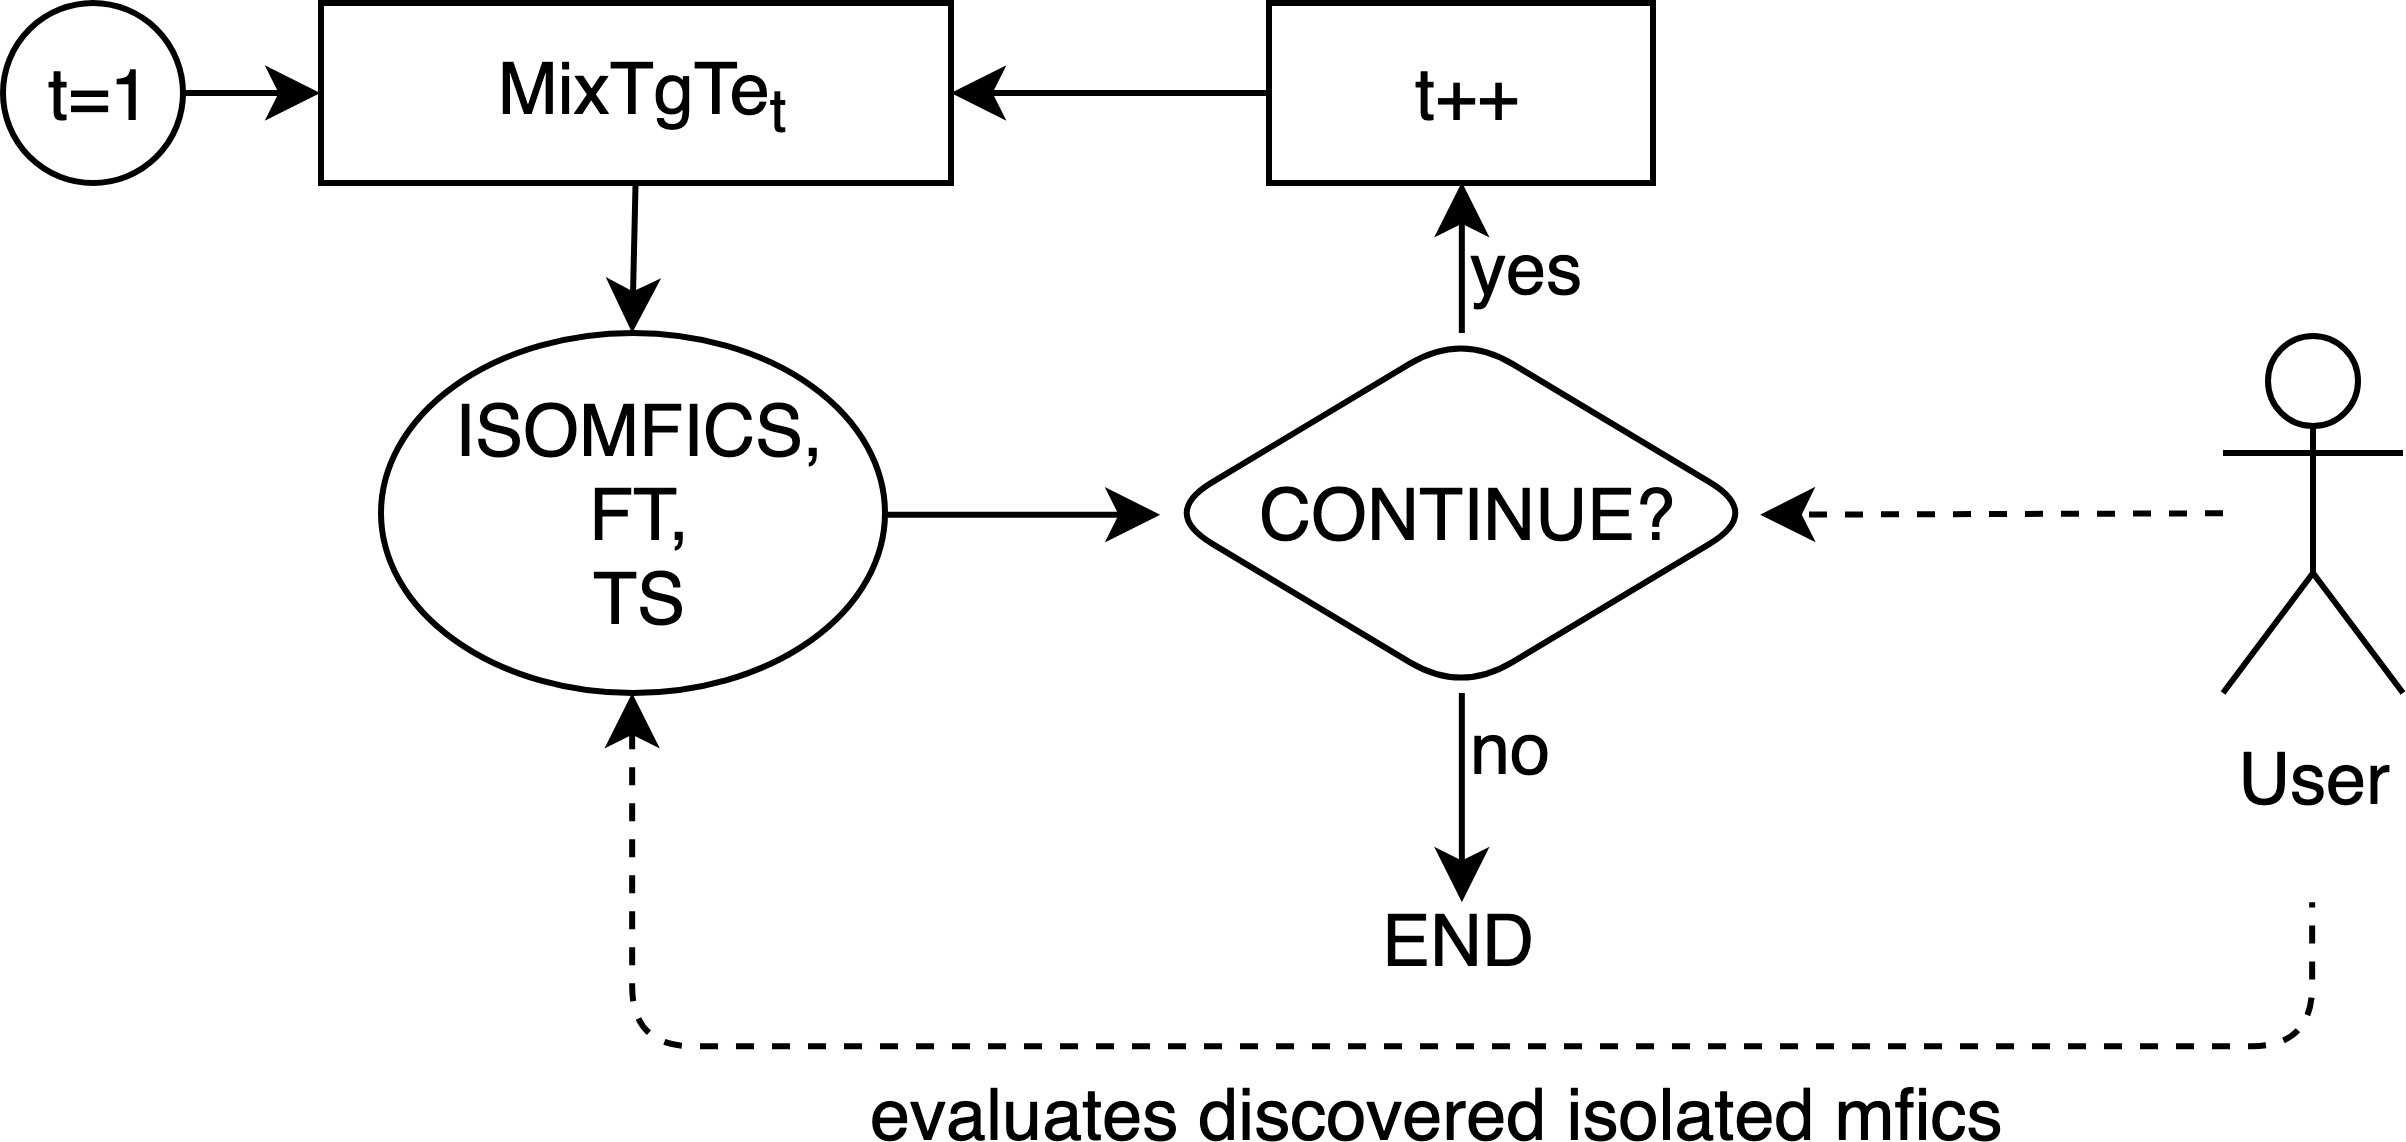
\includegraphics[width=.9\columnwidth]{images/process_mix_fl_tg}
	\caption{Overview of the user-driven iterations of the process alternating test generation and detection of isolated \mfics}
	\label{fig:overallProcess}
\end{figure}
%
\begin{algorithm}[!tb]
	\begin{algorithmic}[1]
		\State{$\isoMficsSet \gets \emptyset$}\label{line:initMFICS}
		\State{$\ft \gets \emptyset$}\label{line:initFT2}
		\State{$\ts \gets \emptyset$}\label{line:initTS}
		\State{$t \gets 1$}\label{line:initT}
		\While{$t \le \vert P \vert \wedge$ User decides to continue}
		\State{\Call{\mixt}{$t, \isoMficsSet, \ts$}}\label{line:call}
		\State{$t \gets t+1$}\label{line:increaseT}
		\EndWhile
		%\State{$mfics \gets mfics \cup \mficst$}
	\end{algorithmic}
	\caption{\mix}
	\label{alg:mix}
\end{algorithm}
%
It starts from identifying combinations of size $t$=1 using the procedure \mixt, and progressively repeats the search algorithm to combinations with higher size, until the user (who, at every iteration, can inspect the set $\isoMficsSet$ of discovered isolated \mfics of size less or equal to $t$) decides to stop the process, or $t$ reaches the number of parameters $\vert P \vert$ of the system under test. The latter condition, however, is equivalent to exercising the exhaustive test suite, and it is normally infeasible in practice, except for trivial systems.

At each step, to keep limited the number of tests to execute on the SUT, the {\it minimal} strength of the test suite used is equal to the size $t$ of the detected combinations. Indeed, by Thm.~\ref{thm:trueMficCTSt}, we can observe that this guarantees to have in the test suite all the \mfics of size $t$. However, it could be some \mfics are not isolated; therefore, at each iteration, we also generate additional tests to isolate all the discovered \mfics.

At each step, the user checks the returned sets of \isoMficsSet to determine if it is the case to continue to search for \mfics of higher strength. The choice to continue or not is based on the available budget, but may also depend on the returned \mfics in \isoMficsSet and the test suite \ts.



\subsection{\mixt}

Fig.~\ref{fig:mixTgFlT} depicts the procedure \mixt that, given a certain combination size $t$, and a set of previously executed tests, produces a combinatorial test suite of strength $t$ able to detect and isolate $\mfics$ of strength up to $t$.
%
\begin{figure}[!tb]
	\centering
	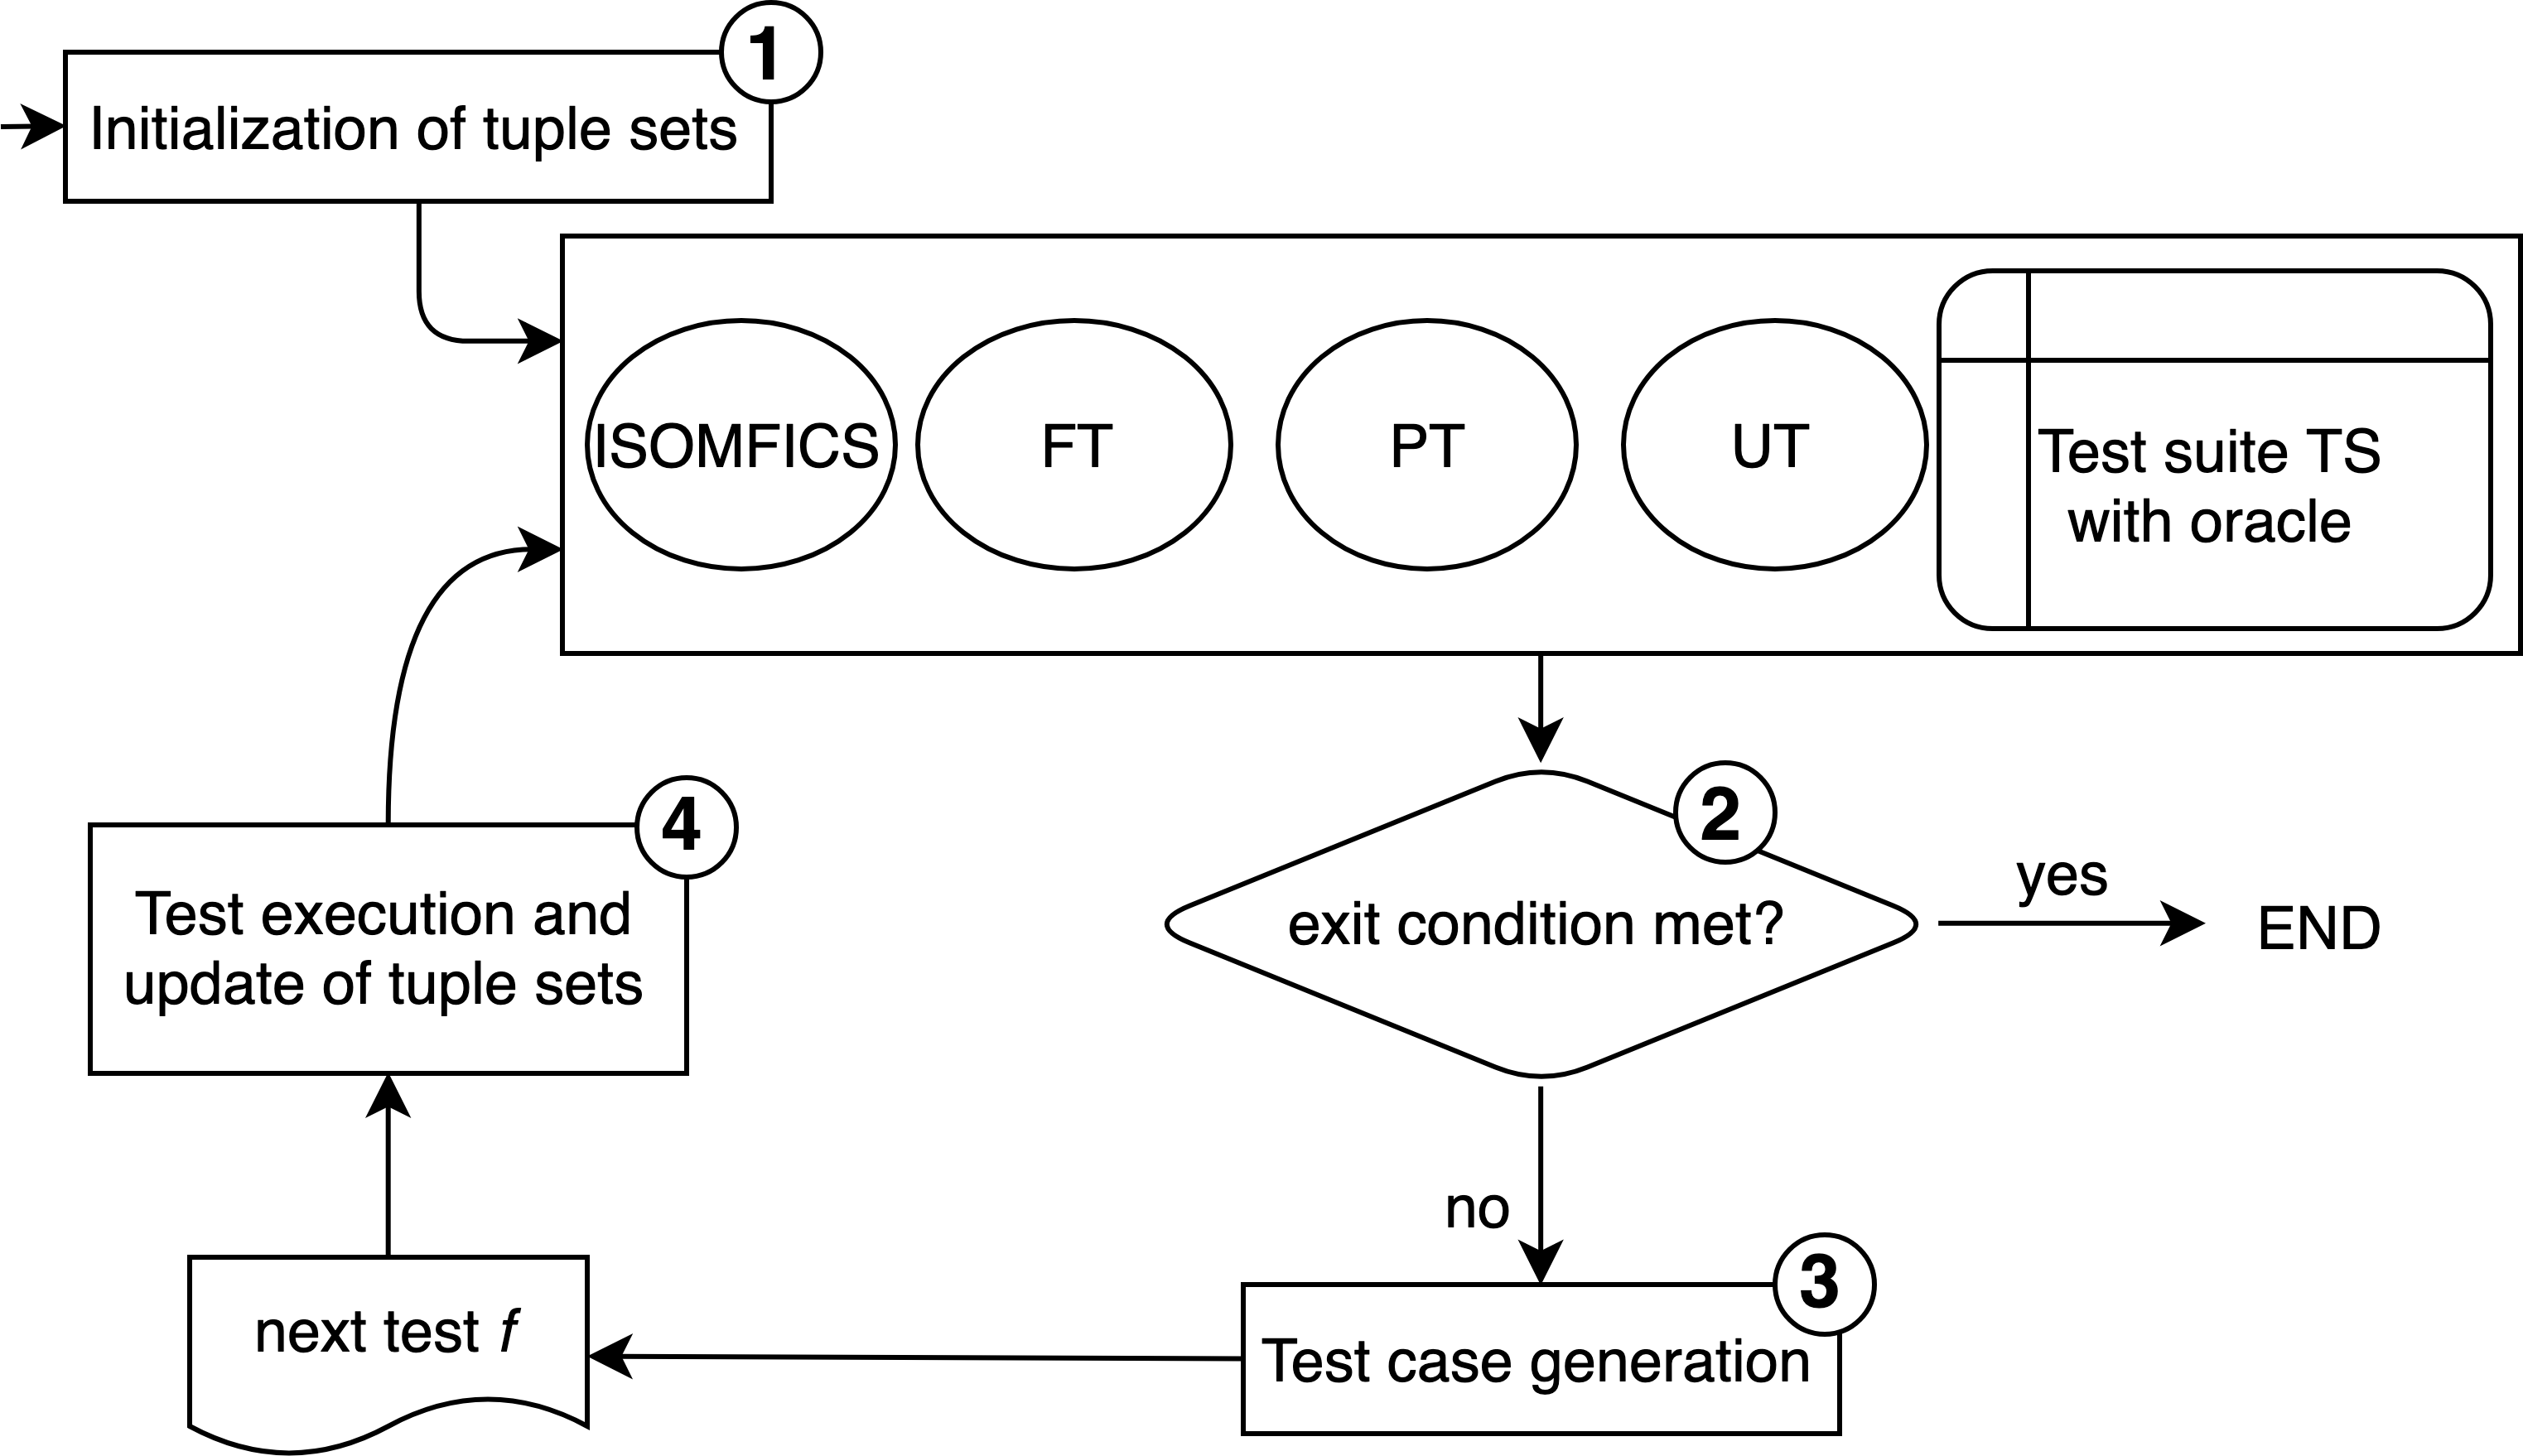
\includegraphics[width=1\columnwidth]{images/process_mix_fl_tg2}
	\caption{\mixt process to find and isolate \mfics up to accuracy of strength $t$}
	\label{fig:mixTgFlT}
\end{figure}
%
The process is described in detail in Alg.~\ref{alg:mixTgFlT} and in the rest of the section.
%
\begin{algorithm}[!tb]
	\begin{algorithmic}[1]
		\Require{$t$: strength}
		\Require{\isoMficsSet: isolated \mfics computed at step $t$-1 (empty if $t$=1)}
		\Require{\ft: failing tuples found at step $t$-1 (empty if $t$=1)}
		\Require{\ts: test suite computed at step $t$-1 (empty if $t$=1)}
		\State{$\pt \gets \{c \subseteq f | f \in \ts \wedge \resultf = \textit{pass} \wedge c \in C_t\}$}\label{line:initPT}
		\State{$\ft \gets \ft \cup \{c \subseteq f | f \in \ts \wedge \resultf = \textit{fail} \wedge c \in C_t\}\setminus \pt$}\label{line:initFT}
		\State{$\ut \gets C_t \setminus (\pt \cup \ft)$}\label{line:initUT}
		%\While{$\neg(\ut=\emptyset \wedge (\ft=\emptyset \vee (\forall c \in \ft, \exists c^\prime \in \isoMficsSet \colon c^\prime \subset c)))$}
		\While{$\neg(\ut=\emptyset \wedge (\ft=\emptyset \vee (\forall c \in \ft \colon \isExplained(c, \ts))))$}
		\State{$f \gets \mathit{buildTest}(\ut, \ft)$}
		\State{$\ts \gets \ts \cup \{f\}$}
		\State{\Call{updateTupleSets}{$f, \pt,\ft, \ut, \isoMficsSet$}}
		\State{\Call{updateMFICS}{$\ts, \ft, \isoMficsSet$}}
		\EndWhile
		%\State{$mfics \gets mfics \cup \mficst$}
	\end{algorithmic}
	\caption{\mixt}
	\label{alg:mixTgFlT}
\end{algorithm}

\mixt works on the following sets of combinations:
%
\begin{itemize}
	\item \textbf{\ut} (Unknown Tuples): the combinations of size $t$ not appeared yet in any test during the process;
	\item \textbf{\pt} (Passing Tuples): the combinations of size $\le t$ that were contained in at least one passing test executed so far in the process;
	\item \textbf{\ft} (Failing Tuples): the combinations of size $\le t$ that were contained only by failing tests, among all the tests executed so far in the process, excluding the isolated \mfics.
	\item \textbf{\isoMficsSet}: the set of isolated \mfics detected so far (of size $\le t$).
\end{itemize}
%
In addition, the process keeps track of the set of tests already run in the test suite \ts, together with the value of their \result (either pass or fail).

We give a further definition that is used in the process.

\begin{defn}[\textbf{Explained \fic}]\label{def:explainedFic}
	Given the set \isoMficsSet and a \fic $c \in \ft$, $c$ is said to be \emph{explained} if it implies one or more isolated \mfics, i.e.,
	%
	\[
	\begin{array}{l}
	\isExplained(c, \isoMficsSet) \equiv\\
	\exists S \in \mathcal{P}(\isoMficsSet) \colon c \rightarrow \bigwedge\limits_{m \in S} m
	\end{array}
	\]
\end{defn}

The rationale is that if a \fic $c$ contains\footnote{Note that, for conciseness, in the definition we use the propositional representation of tuples.} one or more \isoMfics, the failure of the tests $T_c$ in which $c$ fails can be explained. Of course, this is just a heuristic, and some other test could show that actually $c$ is the true \mfic. The definition of explained \fic will be used in the process to balance between {\it exploitation} at strength $t$ and {\it exploration} of higher strengths.



\subsubsection{Tuple sets initialization}
Initially, \pt contains all the tuples of size $t$ that are contained in a passing test of \ts (line~\ref{line:initPT}); \ft, instead, inherits the failing tuples from previous iteration, and is enriched with $t$-tuples that are contained in a failing test, but not in a passing test (line~\ref{line:initFT}). \ut is initialized with the remaining tuples of size $t$ (line~\ref{line:initUT}). \isoMficsSet is kept from the previous step.

\subsubsection{Exit condition}\label{sec:exitCondition}
The process exits as soon as no unknown tuples \ut are present, and either there are no failing tuples or all the failing tuples are {\it explained} (see Def.~\ref{def:explainedFic}), i.e.,
%
\begin{equation}\label{eq:exitCond}
\ut = \emptyset \wedge (\ft=\emptyset \vee (\forall c \in \ft \colon \isExplained(c, \ts)))
\end{equation}

\subsubsection{Test case generation}\label{sec:testGeneration}
If the exit condition is not met (i.e., there is at least an unknown tuple (\ut) or a failing tuple (\ft) that is not explained), the function $\mathit{buildTest}$ generates a test $f$ that contains at least one tuple belonging to either \ut, or to \ft without being explained by any subset of \mfics in \isoMficsSet. The generation works as shown in Alg.~\ref{alg:testGeneration} and described as follows:
%
\begin{algorithm}[!tb]
	\begin{algorithmic}[1]
		\Require{\ts: the tests generated so far}
		\Require{\ut: unknown tuples}
		\Require{\ft: failing tuples}
		\State{$f \gets \emptyset$}
		\If{$\ut \neq \emptyset$}
		\For{$c \in \ut$}\label{line:loopUt}
		\If{$\compatible(c, f)$}\label{line:compatible}
		\State{$f \gets f \cup c$}
		\EndIf
		\If{$\mathit{isCompleteTest(f)}$}
		\State \Return{$f$}
		\EndIf
		\EndFor
		\State{$f \gets \mathit{completeRnd}(f)$}\label{line:completeRnd}
		\State \Return{$f$}\label{line:returnTestUt}
		\Else
		\State{$c_{\mathit{ne}} \gets \mathit{pickRnd}(\{c \in \ft | \neg \isExplained(c, \ts)\})$}\label{line:selectUnexplained}
		\State{$\phi \gets c_{\mathit{ne}} \wedge \bigwedge_{\{f \in \ts | c_{\mathit{ne}} \subseteq f}\} \neg f$}\label{line:initPhi}
		\State{\Return$\mathtt{getModel}(\phi)$}\Comment{A test is a satisfying assignment}\label{line:satPhi}
		\EndIf
	\end{algorithmic}
	\caption{\textsc{buildTest}: Test case generation}
	\label{alg:testGeneration}
\end{algorithm}
%
\begin{compactitem}
	\item if \ut is not empty, we merge together as many tuples $c \in \ut$ as possible (lines~\ref{line:loopUt}-\ref{line:returnTestUt}). Two tuples $c$ and $c^\prime$ cannot be merged if, for a given parameter $p_i$, $p_i$ has different values in $c$ and in $c^\prime$ (this is captured by predicate \compatible at line~\ref{line:compatible}). If after this phase some parameters have no associated value, we randomly generate values for them (line~\ref{line:completeRnd});
	\item if instead \ut is empty, we randomly select a not-explained failing tuple $c$ (line~\ref{line:selectUnexplained}); then, in lines~\ref{line:initPhi}-\ref{line:satPhi} we ask the SMT solver to find a test that contains $c$, but it is different from previous tests in \ts (this is guaranteed to exist, as shown in Thm.~\ref{thm:testGen}).
\end{compactitem}


\subsubsection{Test execution and tuple sets update}

After each test $f$ is generated, it is immediately executed, and, depending on the \result (pass/fail), the tuple sets are updated as described in Alg.~\ref{alg:tupleSetsUpdate}:
%
\begin{algorithm}[!tb]
	\begin{algorithmic}[1]
		\Require{$f$: a test}
		\If{$\resultf$ = {\it fail}}
		\State{\Call{Move}{$f$, \ut, \ft}}
		\Else
		\State{\Call{Move}{$f$, \ut, \pt}}\label{line:moveUT}
		\State{\Call{Move}{$f$, \ft, \pt}}\label{line:moveFT}
		\State{\Call{Move}{$f$, \isoMficsSet, \pt}}\label{line:moveMfics}
		\EndIf
		
		\vspace{10pt}
		\Procedure{move}{$f$, $\sourceSet$, $\destSet$}
		\State{$\toMove \gets \{(c \in \sourceSet) | c \subseteq f\}$}
		\State{$\sourceSet \gets \sourceSet \setminus \toMove$}
		\State{$\destSet \gets \destSet \cup \toMove$}
		\EndProcedure
	\end{algorithmic}
	\caption{\textsc{updateTupleSets}: Tuple sets update}
	\label{alg:tupleSetsUpdate}
\end{algorithm}
%
\begin{compactenum}
	\item If the test $f$ fails, all combinations that are contained both in $f$ and in the set \ut, are moved from \ut to \ft;
	\item If the test passes, we can exploit Obs.~\ref{obs:notFailureInd} and modify the sets as follows:
	\begin{compactenum}
		\item all combinations that are contained both in $f$ and in the set \ut, are moved from \ut to \pt (line~\ref{line:moveUT});
		\item all combinations that are contained both in $f$ and in the set \ft, are moved from \ft to \pt (line~\ref{line:moveFT});
		\item all combinations that are contained both in $f$ and in the set \isoMficsSet, are moved from \isoMficsSet to \pt (line~\ref{line:moveMfics}).
	\end{compactenum}
\end{compactenum}

At this point, we can evaluate whether there are new isolated \mfics, with the procedure shown in Alg.~\ref{alg:isomficsSetUpdate}.
%
\begin{algorithm}[!tb]
	\begin{algorithmic}[1]
		%\Procedure{updateMFICS}{}
		\Require{\ts: the tests generated so far}
		\Require{\isoMficsSet: isolated \mfics}
		\Require{\ft: failing tuples}
		
		\For{$c \in \ft$}
		\If{$\isIsoMfic(c, \ts)$}
		\State{$\ft \gets \ft \setminus \{c\}$}
		\State{$\isoMficsSet \gets \isoMficsSet \cup \{c\}$}
		\EndIf
		\EndFor
		%\EndProcedure
	\end{algorithmic}
	\caption{\textsc{updateMFICS}: \isoMficsSet set update}
	\label{alg:isomficsSetUpdate}
\end{algorithm}
%
If a tuple $c \in \ft$ turns out to be the only one (amongst all the possible tuples) to explain the failure of a test $f$ (i.e., it is isolated in $f$ according to Def.~\ref{def:isolatedMfic}), it is added to \isoMficsSet.

In summary, the status evolution of a combination $c$ is depicted in the state machine shown in Fig.~\ref{fig:tupleLifeCycle}.
%
\begin{figure}[!tb]
	\centering
	\vspace{-50pt}
	\resizebox{0.8\columnwidth}{!}{
		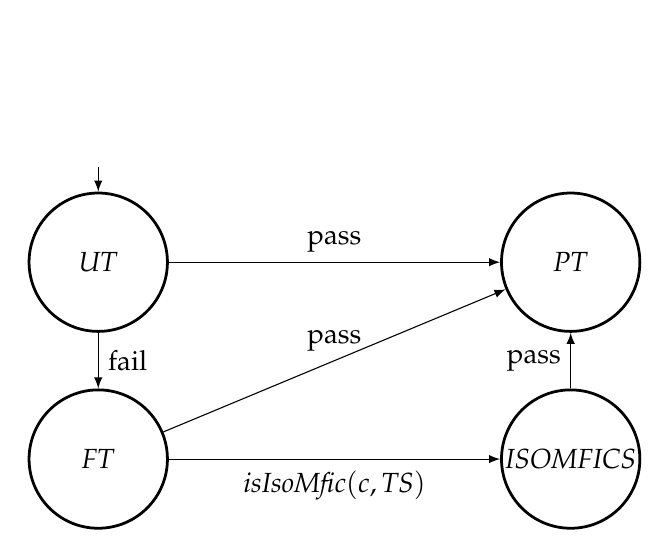
\begin{tikzpicture}
		\tikzstyle{vertex}=[circle, minimum size=50pt,inner sep=0pt, line width=1pt, draw]
		\node[vertex, draw=none] (EMPTY) at (-1,5.1) {};
		\node[vertex, circle] (UT) at (-1,3) {\ut};
		\node[vertex, circle] (PT) at (5,3) {\pt};
		\node[vertex, circle] (FT) at (-1,0.5) {\ft};
		%\node[vertex, circle] (REM) at (-2,-2) {removed};
		\node[vertex, circle] (MFIC) at (5,0.5) {\isoMficsSet};
		\draw[->, >=latex] (EMPTY) -- (UT);
		\draw[->, >=latex] (UT) -- node[above] {pass} (PT);
		\draw[->, >=latex] (UT) -- node[right] {fail} (FT);
		\draw[->, >=latex] (FT) -- node[above] {pass} (PT);
		%\draw[->, >=latex] (PT) -- node[left] {$t$++} (REM);
		%\draw[->, >=latex] (FT) -- node[below left] {$t$++} (REM);
		\draw[->, >=latex] (MFIC) -- node[left] {pass} (PT);
		%\draw[->, >=latex] (FT) -- node[below] {\makecell{$\exists f \in \ts \colon c \subseteq f$ $\wedge \neg \result(f) \wedge$ \\ $ (\forall (c^\prime \subset f) \colon \mathit{size}(c^\prime)=t \rightarrow c^\prime \in \pt))$}} (MFIC);
		\draw[->, >=latex] (FT) -- node[below] {\makecell{$\isIsoMfic(c, \ts)$}} (MFIC);
		\end{tikzpicture}
	}
	\caption{Status evolution of a tuple $c$ throughout the process}
	\label{fig:tupleLifeCycle}
\end{figure}


\begin{example}
	On model $M$ presented in Ex.~\ref{ex:model}, if the \truemfics were $A$ and $B\bar{C}$, a possible trace table of the process, with tests separated by the incremental maximum strength $t$, would be the one presented in Table~\ref{table:genExample} (the scenario with test 8a).
	%
	\begin{table*}[!tb]
		\centering
		\caption{Example of \mix for detecting $\mfics$ of different sizes with a strength up to $t=3$}
		\label{table:genExample}
		\setlength\tabcolsep{1pt}
		\vspace{2mm}
		\def\arraystretch{1.5}\tabcolsep=4pt
		\resizebox{\textwidth}{!}{%
			\begin{tabular}{c|lc|c|c||c|c|c|c|c}
				\toprule
				& \# & A & B & C & \result & \isoMficsSet & \ft & \pt & \ut \\
				\midrule
				\multirow{5}{*}{\rotatebox{90}{$t=1$}}& & \multicolumn{4}{c}{Fill FT-PT-UT} & $\{\}$ & $\{\}$ & $\{\}$ & $\{A, B, C, \bar{A}, \bar{B}, \bar{C}\}$\\ 
				\cline{2-10} 
				& 1& 0 & 0 & 0 & pass & $\{\}$ & $\{\}$ & $\{\bar{A}, \bar{B}, \bar{C}\}$ & $\{A, B, C\}$\\
				%2& 0 & 1 & 1 & pass & $\{\}$ & $\{\}$ & $\{\bar{A}, \bar{B}, \bar{C}, B, C\}$ & $\{A\}$\\
				%3 & \cellcolor{yellow}1 & 1 & 1 & fail & $\{\}$ & $\{A\}$ & $\{\bar{A}, \bar{B}, \bar{C}, B, C\}$ & $\{\}$\\
				& 2 & 1 & 1 & 1 & fail & $\{\}$ & $\{A, B, C\}$ & $\{\bar{A}, \bar{B}, \bar{C}\}$ & $\{\}$\\
				& 3 & 0 & 1 & 1 & pass & $\{\}$ & $\{A\}$ & $\{\bar{A}, \bar{B}, \bar{C}, B, C\}$ & $\{\}$\\
				& \multicolumn{5}{l}{updatedMfics} & $\{A\}$ & $\{\}$ & $\{\bar{A}, \bar{B}, \bar{C}, B, C\}$ & $\{\}$\\
				\midrule
				\multirow{5}{*}{\rotatebox{90}{$t=2$}}%& & \multicolumn{8}{l}{Compute all 2-way tuples} \\%& $\{AB, AC, \bar{A}\bar{B}, \bar{A}\bar{C}, \bar{B}\bar{C}, \bar{A}B, \bar{A}C, BC, A\bar{B}, A\bar{C}, \bar{B}C, B\bar{C}\}$\\
				& & \multicolumn{4}{c}{Fill FT-PT-UT} & $\{A\}$ & $\{AB, AC\}$ & $\{\bar{A}\bar{B}, \bar{A}\bar{C}, \bar{B}\bar{C}, \bar{A}B, \bar{A}C, BC\}$ & $\{A\bar{B}, A\bar{C}, \bar{B}C, B\bar{C}\}$\\
				\cline{2-10}
				& 4& 1 & 0 & 0 & fail & $\{A\}$ & $\{AB, AC, A\bar{B}, A\bar{C}\}$ & $\{\bar{A}\bar{B}, \bar{A}\bar{C}, \bar{B}\bar{C}, \bar{A}B, \bar{A}C, BC\}$ & $\{B\bar{C}, \bar{B}C\}$\\
				%& 5 & 1 & 1 & 0 & fail & $\{A\}$ & $\{AB, AC, \bar{B}C, A\bar{B}, A\bar{C},B\bar{C}\}$ & $\{\bar{A}\bar{B}, \bar{A}\bar{C}, \bar{B}\bar{C}, \bar{A}B, \bar{A}C, BC\}$ & $\{\}$\\
				& 5 & 0 & 1 & 0 & fail & $\{A\}$ & $\{AB, AC, A\bar{B}, A\bar{C},B\bar{C}\}$ & $\{\bar{A}\bar{B}, \bar{A}\bar{C}, \bar{B}\bar{C}, \bar{A}B, \bar{A}C, BC\}$ & $\{\bar{B}C\}$\\
				& \multicolumn{5}{l}{updatedMfics} & $\{A, B\bar{C}\}$ & $\{AB, AC, A\bar{B}, A\bar{C}\}$ & $\{\bar{A}\bar{B}, \bar{A}\bar{C}, \bar{B}\bar{C}, \bar{A}B, \bar{A}C, BC\}$ & $\{\bar{B}C\}$\\
				
				& 6& 0 & 0 & 1 & pass & $\{A, B\bar{C}\}$ &$\{AB, AC, A\bar{B}, A\bar{C}\}$ & $\{\bar{A}\bar{B}, \bar{A}\bar{C}, \bar{B}\bar{C}, \bar{A}B, \bar{A}C, BC, \bar{B}C\}$ & $\{\}$\\
				%-- & -- & -- & -- & -- & $\{A, B\bar{C}\}$ & $\{\}$ & $\{\bar{A}\bar{B}, \bar{A}\bar{C}, \bar{B}\bar{C}, \bar{A}B, \bar{A}C, BC, \bar{B}C\}$ & $\{\}$\\
				
				\midrule
				\multirow{7}{*}{\rotatebox{90}{$t=3$}} %& & \multicolumn{8}{l}{Compute all 3-way tuples} \\
				& & \multicolumn{4}{c}{Fill FT-PT-UT} & $\{A, B\bar{C}\}$ &$\{AB, AC, A\bar{B}, A\bar{C}, ABC, \bar{A}B\bar{C}, A\bar{B}\bar{C}\}$ & $\{\bar{A}\bar{B}\bar{C}, \bar{A}BC, \bar{A}\bar{B}C\}$ & $\{A\bar{B}C, AB\bar{C}\}$\\
				
				\cline{2-10}
				& 7 & 1 & 0 & 1 & fail & $\{A, B\bar{C}\}$ & $\{AB, AC, A\bar{B}, A\bar{C}, A\bar{B}C, A\bar{B}\bar{C}, ABC, \bar{A}B\bar{C}\}$ & $\{\bar{A}\bar{B}\bar{C}, \bar{A}BC, \bar{A}\bar{B}C\}$ & $\{AB\bar{C}\}$\\
				
				\cline{2-10}
				& \multicolumn{6}{c}{a) Scenario in which test 8 fails} \\
				& 8a & 1 & 1 & 0 & fail & $\{A, B\bar{C}\}$ & $\{AB, AC, A\bar{B}, A\bar{C}, A\bar{B}C, A\bar{B}\bar{C}, ABC, \bar{A}B\bar{C}, AB\bar{C}\}$ & $\{\bar{A}\bar{B}\bar{C}, \bar{A}BC, \bar{A}\bar{B}C\}$ & $\{\}$\\
				%& \multicolumn{5}{l}{updatedMfics} & $\{A, B\bar{C}\}$ & $\{\}$ & $\{\bar{A}\bar{B}\bar{C}, \bar{A}BC, \bar{A}\bar{B}C\}$ & $\{\}$\\
				
				\cline{2-10}
				& \multicolumn{6}{c}{b) Scenario in which test 8 passes} \\
				& 8b & 1 & 1 & 0 & pass & $\{\}$ & $\{A\bar{B}, AC, A\bar{B}C, A\bar{B}\bar{C}, ABC, \bar{A}B\bar{C}\}$ & $\{A, B\bar{C}, AB, A\bar{C}, \bar{A}\bar{B}\bar{C}, \bar{A}BC, \bar{A}\bar{B}C, AB\bar{C}\}$ & $\{\}$\\
				& \multicolumn{5}{l}{updatedMfics} & $\{A\bar{B}, AC, \bar{A}B\bar{C}\}$ & $\{A\bar{B}C, A\bar{B}\bar{C}, ABC \}$ & $\{A, B\bar{C}, AB, A\bar{C}, \bar{A}\bar{B}\bar{C}, \bar{A}BC, \bar{A}\bar{B}C, AB\bar{C}\}$ & $\{\}$\\
				\bottomrule
			\end{tabular}
		}
	\end{table*}
	%
	We observe that the \truemfics have been correctly identified with the first two executions of \mixt (till test 6), i.e., tests 7 and 8a (for strength $t$=3) are not necessary, since the maximum strength of the \truemfics is 2.
	
	Instead, if the true \mfics were $A\bar{B}$, $AC$, and $\bar{A}B\bar{C}$, the process should be run three times for correctly identifying them (using test 8b), since there is a \truemfic of size 3.
\end{example}


\section{Properties of the \mix process}\label{sec:theorems}

In this section, we introduce some theorems assessing the capabilities of the proposed process.

We first make an assumption that is needed for our process.

%\begin{assumption}\label{assu:oneTestEts}
%There is at least one passing test in \ets.\todo{Proposta: questo diventa: "All \truemfics can be isolated."}
%\end{assumption}

%The existence of at least one passing test is needed for guaranteeing that \mfics can be isolated (see Thm.~\ref{thm:isolatedMfic}). Note that it is unlikely that a system fails on every possible input.

\begin{assumption}\label{assu:oneTestEts}
	All \truemfics can be isolated.
\end{assumption}

\begin{thm}[Test case generation]\label{thm:testGen}
	In the test case generation (see Sect.~\ref{sec:testGeneration}), it is always possible to generate a test case.
\end{thm}

\begin{proof}
	When \ut is not empty, the test $f$ is generated by merging compatible tuples from \ut and then randomly selecting values for other parameters; since tuples in \ut are those that have never been observed in any test, the new test $f$ is guaranteed to exist. When \ut is empty, the generated test must be an assignment satisfying formula $\phi$ at line~\ref{line:initPhi} of Alg.~\ref{alg:testGeneration}. Let's assume that such test does not exist; it would mean that all the possible tests $T_{c_{\mathit{ne}}}$ containing $c_{\mathit{ne}}$ have already been generated; there would be two cases:
	%
	\begin{compactitem}
		\item at least one of the tests in $T_{c_{\mathit{ne}}}$ passes; this is not possible, as, in this case, $c_{\mathit{ne}}$ would be in \pt;
		\item all the tests in $T_{c_{\mathit{ne}}}$ fail; also this is not possible, as, in this case, $c_{\mathit{ne}}$ would be either in \isoMficsSet or explained by a subset of tuples in \isoMficsSet.%\todo{NON E' VERO!}
	\end{compactitem}
\end{proof}

\begin{thm}[Termination]\label{thm:termination}
	The process is guaranteed to terminate.
\end{thm}

\begin{proof}
	The outer process \mix terminates when the \textit{user} (i.e., the test engineer) decides not to continue it, or when $t=\vert P \vert$.
	
	The inner process \mixt terminates when the exit condition (see Eq.~\ref{eq:exitCond}) is met. The test generation phase (see Sect.~\ref{sec:testGeneration}) directly aims at emptying \ut and explaining all the not explained tuples in \ft. Since, by Thm.~\ref{thm:testGen}, the generation is always possible, the exit condition will be eventually met.
\end{proof}

We want to prove that, under the assumption that the SUT has only true \mfics of limited strength, by running the process till that strength, we will find them.

\begin{assumption}\label{assu:maxStrength}
	Each true-\mfic has maximum strength $t$.
\end{assumption}

\begin{thm}[True-\mfics found]\label{thm:trueMficsFound}
	If \trueMficsSet is the set of true \mfics and each $c$ in \trueMficsSet has maximum strength $t$, then by running the process with strength equal or greater than $t$, \isoMficsSet is equal to \trueMficsSet.
\end{thm}

\begin{proof}
	Under the stated assumption, the property is twofold: if $c$ is a \truemfic, the \mix will find it and if the \mix finds a $c$ as \mfic, then $c$ is a \truemfic.
	%
	\begin{compactenum}
		\item If $c$ is a \truemfic then \isoMficsSet will contain $c$. Let's assume that $c$ is a \truemfic but \isoMficsSet does not contain it at the end. By Thm.~\ref{thm:trueMficCTSt}, $c$ is contained in a failing test of \ts and so it is in \ft at a given point. When the process terminates, \ft is either empty (and so $c$ is in \isoMficsSet), or all the tuples in \ft are explained (by Def.~\ref{def:explainedFic}), i.e., they contain one or more \isoMfic. However, the latter case is not possible, as $c$ would not be minimal.
		\item If $c$ is in \isoMficsSet, it is a \truemfic. Let's assume that $c$ is in \isoMficsSet, but it's not a \truemfic. If $c$ is in \isoMficsSet, all tests containing it fail, and there exists a test in which it is the only \mfic; if it is not a \truemfic, it means that in each test containing $c$ there must be a combination $c^\prime$ such that $c \subset c^\prime$ and $c^\prime$ is a \truemfic and, therefore, added to \isoMficsSet by point 1: in this case, $c^\prime$ would violate the minimality requirement. Note that, if $c$ has size $t$, there cannot be a \truemfic $c^\prime$ of higher strength containing $c$ by Assumption~\ref{assu:maxStrength}.
	\end{compactenum}
\end{proof}


\section{Evaluation}\label{sec:evaluation}

In this section, we evaluate the process and we compare it with other techniques for fault interaction detection.

\subsection{Benchmarks}\label{sec:benchmarks}

%For the experiments, we selected some benchmarks, each one constituted by two combinatorial models with constraints: $M_f$ representing the faulty version of the SUT, and $M_o$ representing the oracle. Therefore, for each benchmark, we also know the \truemfics in $M_f$. The assessment of the execution of a test $f$ (i.e., \result in Def.~\ref{def:testCase}) is performed by comparing the evaluations of $f$ over $M_f$ and $M_o$.

%For the experiments, we selected some benchmarks, each one constituted by two behavioural models: $M_f$ representing the faulty version of the SUT, and $M_o$ representing the oracle. The assessment of the execution of a test $f$ (i.e., \result in Def.~\ref{def:testCase}) is performed by comparing the evaluations of $f$ over $M_f$ and $M_o$. Therefore, for each benchmark, we also know the \truemfics in $M_f$.
For the experiments, we selected some benchmarks, each one constituted by a faulty version of the SUT $S_f$ and an oracle $O$. The assessment of the execution of a test $f$ (i.e., \result in Def.~\ref{def:testCase}) is performed by comparing the evaluations of $f$ over $S_f$ and $O$. For practicality, we build a combinatorial model $M$ having the same parameters of $S_f$\footnote{Note that $S_f$ and $O$ have the same parameters and they only differ on the behaviour.} and constraints that accept only the tests for which $S_f$ and $O$ agree (the constraints are the negation of the \truemfics).\footnote{Note that these constraints are not related to the combinatorial problem that, as stated in Sect.~\ref{sec:background}, is unconstrained in our setting.} Therefore, for each benchmark, we also know the \truemfics in $S_f$.

We used two sets of benchmarks described in Table~\ref{table:benchmarks}.
%
\begin{table}[!tb]
	\centering
	\caption{Benchmark properties}
	\label{table:benchmarks}
	%\resizebox{\columnwidth}{!}{%
	%\setlength\tabcolsep{1pt}
	\begin{tabular}{c|cccr} 
		\toprule
		& name & $\vert P \vert$ & size & \trueMficsSet\\
		& & & & \multicolumn{1}{c}{(size (\#))}\\
		\midrule
		\multirow{8}*{\rotatebox{90}{\small \benchArt}}
		&{\tt runExA} & 3 & $2^3$ & 1(1), {\bf 2}(1)\\
		&{\tt runExB} & 3 & $2^3$ & 2(2), {\bf 3}(1)\\
		&{\tt art1} & 3 & $2^3$ & {\bf 2}(1)\\
		&{\tt art2} & 3 & $2^3$ & {\bf 2}(2)\\
		&{\tt art3} & 3 & $2^3$ & 1(1), {\bf 2}(1)\\
		&{\tt art4} & 7 & $2^7$ & 2(1), {\bf 3}(1)\\
		&{\tt art5} & 7 & $2^7$ & {\bf 2}(1)\\
		&{\tt art6} & 5 & $2^3 3^1 5^1$ & {\bf 3}(1) \\
		%& {\tt Django} & 24 & $2^{23} 4^1$ & $1^2 2^2$ \\
		\midrule
		\multirow{5}*{\rotatebox{90}{\small \benchReal}}
		& {\tt aircraft} & 8 & $2^7 3^1$ & 3(1), {\bf 4}(1)\\
		& {\tt tomcat} & 12 & $2^8 3^1 4^1$ & 1(1), {\bf 2}(2)\\
		& {\tt hsqldb} & 10 & $2^9 6^1$ & 1(1), {\bf 3}(2)\\
		& {\tt gcc} & 10 & $2^8 3^1 4^1 $ & {\bf 3}(4)\\
		& {\tt jflex} & 13 & $2^{10} 3^2 4^1 $ & {\bf 2}(1)\\
		\bottomrule
	\end{tabular}
	%}
\end{table}
%
The first benchmark set, \benchArt, is constituted by \textit{artificial} models of systems; we generated some of these models with one \truemfic (\texttt{art1}, \texttt{art5}, and \texttt{art6}), and others with multiple \truemfics. \benchArt also contains the running example, in its two versions shown in Table~\ref{table:genExample}. The second benchmark set, \benchReal, represents real systems: \texttt{aircraft} is a Software Product Line model presented in~\cite{Voelter:2009} and taken from the SPLOT repository\footnote{http://www.splot-research.org/}, and the others four are benchmarks used in Niu et al.~\cite{Niu2018interleaving}.

In Table~\ref{table:benchmarks}, column \textit{size} reports the size of model $M$, presented in the abbreviated form $k^{\# \mathit{params}_k} \times \ldots$, where $k$$\in$$N^+$ and $\mathit{params}_k$ are the parameters having $k$ values; for example, $2^8$$3^1$$4^1$ indicates that the SUT has 8 parameters that can take 2 values, one parameter taking 3 values, and one parameter taking 4 values. Column \trueMficsSet reports the number and size of \truemfics in $M_f$; we report each possible size with the number of \mfics of that size in parentheses. We also mark in bold face the maximum strength of the \truemfic; in the experiments, we assume Assumption~\ref{assu:maxStrength}, and so we apply the approach only up to the known maximal strength (according to Thm.~\ref{thm:trueMficsFound}, this guarantees to find all the \mfics).


\subsection{Compared approaches}\label{sec:processes}

We compare our approach with some existing methods from literature, namely:
%
\begin{asparadesc}
	\item[BEN:] a process based on the first phase of the BEN tool proposed by Ghandehari et al.~\cite{ben_2015}. The process consists in calling BEN for failure-inducing combination detection, by providing an initial combinatorial test suite of a certain strength $t$, and iterating over the size of the failure-inducing combinations to try to detect them. This process has already been used for constraints validation and repair~\cite{Gargantini16:validation,gargantini_combinatorial_2017}. The BEN tool is included in our experimental process as a jar file.
	\item[SOFOT:] the \textit{Simplified One Factor One Time} method to infer the Minimal Failure-causing Schema (\textsf{MFS}) from a given failing test case, from Nie et al.~\cite{nie_2011}. This method takes as input a set of failing tests, and tries to reduce each test to an \mfic. For each failing test $f$, it generates new tests by changing the value of each parameter in $f$ one by one. Note that the source code of this method is available in Python from a later work by Zhang and Zhang~\cite{zhang_characterizing_2011}. As our automated evaluation script is written in Java, we program it so that it calls Python via command line. This causes some overhead which affects the total execution time in the experiments.
	\item[FIC:] the \textit{Faulty Interaction Characterization} method proposed by Zhang et al.~\cite{zhang_characterizing_2011}. It is similar to SOFOT, in the sense that it accepts in input a set of tests known to be failing, and it tries to isolate the minimal failure-inducing combination(s) from it. It proceeds by considering one failing test a time, and changing the value of a parameter at a time, but, unlike SOFOT, it keeps the value changed. Furthermore, it performs a few iterations until the original failing test, with the value of the detected minimal failure-inducing combinations changed, passes. If there are two different failure-inducing combinations in the same tests, it may find them, but without a guarantee to be correct. We made a Java implementation of the algorithm described in the paper~\cite{zhang_characterizing_2011}.
	\item[ICT:] the \textit{Interleaving CT} approach proposed by Niu et al.~\cite{Niu2018interleaving}. It is a significant improvement of SOFOT that alleviates its three main problems: redundant test cases, multiple \mfics, and masking effects (where multiple \mfics are present in the same test). Like SOFOT, it is composed of two phases, generation and identification. Test generation is here made adaptive, one test at a time, in a similar way as the one of our approach. This reduces the amount of tests needed, by forbidding the generation of new tests containing already discovered failure-inducing combinations. The identification phase has a novel feedback checking mechanism (based on information coming from the execution of a few new proposed test cases), which can check, up to a certain extent, whether the identified \mfic is a \truemfic or not; and it significantly improves the accuracy of the results w.r.t. SOFOT. The method is very recent, and, although we could not manage to re-run the tool on new benchmarks, we compared the results of \mix with the results of ICT reported in that paper for a common set of benchmarks.
\end{asparadesc}

Since FIC and SOFOT require failing tests as input, but do not say how to find such failing tests, we need to build a test suite to find such failing tests. In order to try to make the comparison fair, we use, for all the methods\footnote{Note that \mix, BEN, and ICT already require a combinatorial test suite.}, an initial combinatorial test suite $\cts_t$ of strength $t$=$\max\limits_{c \in \trueMficsSet}|\mathit{size}(c)|$, being \trueMficsSet the set of \truemfics (as shown in Table~\ref{table:benchmarks}). 
$\cts_t$ is generated using ACTS\footnote{https://csrc.nist.gov/projects/automated-combinatorial-testing-for-software} for FIC, BEN, and SOFOT. \mix, instead, generates tests in an adaptive way, as described in Sect.~\ref{sec:testGeneration}. ICT, instead, uses AETG~\cite{AETG}.

In the following, \detMficsSet denotes the set of \mfics returned by a method; in our case, it corresponds to \isoMficsSet.

\subsection{Results}\label{sec:results}

We run our method and the compared 4 methods 10 times for each benchmark; results are the average across the runs. Experiments have been executed on a Mac OS X 10.14, Intel Core i3, with 4GB of RAM. Code was written in Java, using CTWedge libraries for combinatorial modeling, test generation, and test execution~\cite{IWCTGargantini2018}. The code and all the benchmarks are available online at https://github.com/fmselab/mixtgte.

Table~\ref{table:resultsByBenchmarkPrecRec} shows the results of the experiments.
%
\begin{table*}[!tb]
	\centering
	\caption{Experimental results (P: precision, R: recall, F: F-score, time is in ms)}
	\label{table:resultsByBenchmarkPrecRec}
	%\resizebox{\columnwidth}{!}{%
	\setlength\tabcolsep{2.1pt}
	\begin{tabular}{c|c|ccccr|ccccr|ccccr|ccccr|ccccr} 
		\toprule
		& model & \multicolumn{5}{c}{$\mix$} & \multicolumn{5}{c}{FIC} & \multicolumn{5}{c}{BEN} & \multicolumn{5}{c}{SOFOT} & \multicolumn{5}{c}{ICT}\\
		& & tests & P & R & F & time & tests & P & R & F & time & tests & P & R & F & time & tests & P & R & F & time & tests & P & R & F & time \\
		\midrule
		\multirow{8}*{\rotatebox{90}{\small \benchArt}}
		&{\tt runExA} & 7.6 & 1 & 1 & 1 & 15.9 & 8 & 1.00 & 1.00 & 1.00 & 0.4 & 7 & 0.20 & 0.50 & 0.29 & 53.2 & 8 & 0.75 & 0.50 & 0.58 & 518 & -- & -- & -- & -- & --\\
		&{\tt runExB} & 8.0 & 1 & 1 & 1 & 4.9 & 8 & 0.75 & 1.00 & 0.86 & 0.6 & 8 & 0.25 & 0.33 & 0.29 & 9.4 & 8 & 0.75 & 1.00 & 0.86 & 735 & -- & -- & -- & -- & --\\
		&{\tt art1} & 6.6 & 1 & 1 & 1 & 3.2 & 5 & 1.00 & 1.00 & 1.00 & 0.5 & 7 & 1.00 & 1.00 & 1.00 & 13.0 & 7 & 1.00 & 1.00 & 1.00 & 269 & -- & -- & -- & -- & --\\
		&{\tt art2} & 8.0 & 1 & 1 & 1 & 5.4 & 7 & 1.00 & 1.00 & 1.00 & 0.6 & 7 & 0.50 & 0.50 & 0.50 & 13.8 & 8 & 0.50 & 0.50 & 0.50 & 396 & -- & -- & -- & -- & -- \\
		&{\tt art3} & 7.6 & 1 & 1 & 1 & 2.7 & 8 & 1.00 & 1.00 & 1.00 & 0.7 & 7 & 0.00 & 0.00 & -- & 15.1 & 8 & 1.00 & 0.50 & 0.67 & 403 & -- & -- & -- & -- & --\\
		&{\tt art4} & 36.9 & 1 & 1 & 1 & 79.7 & 29 & 0.67 & 1.00 & 0.80 & 1.8 & 26 & 0.00 & 0.00 & -- & 64.8 & 61 & 1.00 & 1.00 & 1.00 & 2772 & -- & -- & -- & -- & --\\
		&{\tt art5} & 14.7 & 1 & 1 & 1 & 5.0 & 12 & 1.00 & 1.00 & 1.00 & 0.5 & 18 & 1.00 & 1.00 & 1.00 & 14.1 & 20 & 1.00 & 1.00 & 1.00 & 769 & -- & -- & -- & -- & --\\
		&{\tt art6} & 45.4 & 1 & 1 & 1 & 17.1 & 35 & 0.50 & 1.00 & 0.67 & 3.2 & 38 & 1.00 & 1.00 & 1.00 & 21.1 & 52 & 1.00 & 1.00 & 1.00 & 1830 & -- & -- & -- & -- & --\\
		%& {\tt Django} & -- & -- & -- & -- \\
		\midrule
		\multirow{5}*{\rotatebox{90}{\small \benchReal}}
		& {\tt aircraft} & 89.8 & 1 & 1 & 1 & 156.5 & 71 & 1.00 & 1.00 & 1.00 & 18.4 & 62 & 0.00 & 0.00 & -- & 56.4 & 115 & 1.00 & 1.00 & 1.00 & 4157 & -- & -- & -- & -- & --\\
		%& {\tt totinfo} & 269 & -- & 191 & --\\
		%& {\tt printtokens2} & -- & -- & -- & --\\
		%& {\tt schedule} & -- & -- & -- & --\\
		& {\tt gcc} & 88.5 & 1 & 1 & 1 & 134.5 & 64 & 0.50 & 0.50 & 0.50 & 8.9 & 60 & 1.00 & 0.50 & 0.67 & 56.1 & 142 & 0.75 & 0.75 & 0.75 & 4934 & 89.0 & 0.77 & 0.65 & 0.70 & 1118 \\
		&{\tt hsqldb} &169.8 & 1 & 1 & 1 & 3752.8 & 97 & 1.00 & 1.00 & 1.00 & 36.6 & 55 & 0.00 & 0.00 & -- & 532.2 & 443 & 1.00 & 0.67 & 0.80 & 19612 & 88.3 & 1.00 & 1.00 & 1.00 & 2094 \\
		&{\tt jflex} & 22.9 & 1 & 1 & 1 & 9.1 & 15 & 1.00 & 1.00 & 1.00 & 1.6 & 23 & 1.00 & 1.00 & 1.00 & 15.2 & 31 & 1.00 & 1.00 & 1.00 & 978 & 31.6 & 1.00 & 1.00 & 1.00 & 187 \\
		&{\tt tomcat} & 65.9 & 1 & 1 & 1 & 111.9 & 28 & 0.67 & 0.67 & 0.67 & 4.1 & 23 & 0.00 & 0.00 & -- & 31.5 & 128 & 1.00 & 1.00 & 1.00 & 5675 & 128 & 1.00 & 1.00 & 1.00 & 5671 \\
		%& {\tt Connector} & 20 & 20 \\
		\midrule
		& Average & 44.0 & 1 & 1 & 1 & 331 & 29.8 & 0.85 & 0.94 & 0.88 & 5.99 & 26.2 & 0.46 & 0.45 & 0.44 & 68.9 & 79.3 & 0.90 & 0.84 & 0.86 & 3311 & 67.4 & 0.94 & 0.91 & 0.92 & 988 \\
		\bottomrule
	\end{tabular}
	%}
\end{table*}
%
For each method, it reports the total number of different tests required to complete the detection\footnote{If a test is generated twice by a method, we count it only once.}, and the execution time in milliseconds. Moreover, in order to measure the {\it quality} of the returned \mfics, we use classical measures as {\it precision} (P), {\it recall} (R), and {\it F-score} (F). Precision is defined as:
%
\[\mathit{precision} = \frac{|\detMficsSet \cap \trueMficsSet|}{|\detMficsSet|}\]
%
Precision measures the percentage of found \mfics that are \truemfics. If precision is not 1, the developer will spend some time in doing fault localization for a \fic that is not a \truemfic (those in $\detMficsSet \setminus\trueMficsSet$).

Recall is defined as:
%
\[\mathit{recall} = \frac{|\detMficsSet \cap \trueMficsSet|}{|\trueMficsSet|}\]
%
It measures how many \truemfics are actually identified. If the recall is not 1, the developer is not aware of a \truemfic that causes a fault (those in $\trueMficsSet \setminus \detMficsSet$).

The F-measure is the combination of precision and recall, defined as follows:
%
\[\textnormal{\it F-score} = \frac{2 \times \mathit{precision} \times \mathit{recall}}{\mathit{precision} + \mathit{recall}}\]

We now evaluate the approach answering the following three research questions.

\researchquestion{How is the effectiveness (in terms of precision and recall) of \mix w.r.t. other techniques?}

From the results presented in Table~\ref{table:resultsByBenchmarkPrecRec}, we observe that \mix always achieves maximum precision and recall; this is expected, as Thm.~\ref{thm:trueMficsFound} guarantees that, under the assumption that we know the maximum strength $t$, executing \mix till strength $t$ produces an \isoMficsSet set (i.e., \detMficsSet) equal to \trueMficsSet. All the other techniques do not provide this theoretical guarantee.

Among the other methods, ICT has the highest values for precision, recall, and \fScore (92\% on average) on the 4 available benchmarks~\cite{Niu2018interleaving}. For 3 benchmarks, ICT correctly identified all the \trueMficsSet; only for \textit{gcc}, some are wrongly identified (precision 77\%) and some are not found (recall 65\%).

Also FIC and SOFOT showed to be able to correctly identify the \truemfics in many occasions, although not with the same overall accuracy as ICT in terms of \fScore (88\% and 86\%). We believe that this is due not only to the fixed amount of tests asked for the \textit{identification} phase of those methods (they change always one parameter at a time, and only once), but also to the \textit{masking effect}, i.e., when there are two \mfics present in a same test. This effect may happen in general, as explained in Thm.~\ref{thm:insufficientAccuracyCTSt}. As an example of this fact, consider the running example described in Ex.~\ref{ex:model} and the test suite generated by SOFOT shown in Table~\ref{table:executionSOFOT}.
%
\begin{table}[!tb]
	\centering
	\caption{Execution trace of SOFOT on example SUT}
	\label{table:executionSOFOT}
	%\resizebox{.8\columnwidth}{!}{%
	\begin{tabular}{r|c|c|c||c}
		\multicolumn{5}{c}{Generation of $\cts_2$ with ACTS (to have some failing test)}\\
		\toprule
		%\multicolumn{5}{c}{2-way combinatorial coverage to find the faults} \\
		%\midrule
		\# & A & B & C & \result \\
		\hline 
		%& \multicolumn{4}{c}{1-way combinatorial coverage to find the faults} \\
		%1& 1 & 0 & 0 & \textsf{pass} \\
		%2& 0 & 1 & 1 & \textsf{pass} \\
		%\hline
		%1& 1 & 1 & 0 & \textsf{fail} $\vartriangleleft$ fault \ding{172} detected\\
		1& 1 & 1 & 0 & failing test \ding{172}\\
		%2& 1 & 0 & 1 & \textsf{fail} $\vartriangleleft$ fault \ding{173} detected\\
		2& 1 & 0 & 1 & failing test \ding{173}\\
		3& 0 & 1 & 1 & \textsf{pass} \\
		4& 0 & 0 & 0 & \textsf{pass} \\
		\bottomrule
		\multicolumn{5}{c}{}\\
		\multicolumn{5}{c}{}\\ 
		\multicolumn{5}{c}{Identification by SOFOT (tests added to find \mfics)} \\
		\toprule
		\multicolumn{5}{c}{additional tests for failing test \ding{172}} \\
		\midrule
		\# & A & B & C & \result \\
		\hline
		5& 0 & 1 & 0 & \textsf{fail} \\
		6& 1 & 0 & 0 & \textsf{fail} \\
		7& 1 & 1 & 1 & \textsf{fail} \\
		\multicolumn{5}{c}{No \mfic found}\\ 
		\hline
		\multicolumn{5}{c}{} \\
		\hline
		\multicolumn{5}{c}{additional tests for failing test \ding{173}}\\
		\midrule
		\# & A & B & C & \result \\
		\hline
		8& 0 & 0 & 1 & \textsf{pass} \\
		--& 1 & 1 & 1 & \textsf{fail} \\
		--& 1 & 0 & 0 & \textsf{fail} \\
		\multicolumn{5}{c}{$A$ identified as \mfic}\\ 
		\bottomrule
	\end{tabular}
	%}
\end{table}
%
Let's recall that the SUT is made of three binary parameters \{A, B, C\}, with two \truemfics, $A$ and $B\bar{C}$. By providing to SOFOT the faulty test cases observed with a combinatorial test suite of strength $t=2$ (that it is also the maximum strength of the \truemfics, so the correct settings for the experiments) generated with ACTS, the SOFOT method is able to correctly identify only the \mfic $A$. Table~\ref{table:executionSOFOT} reports, at the beginning, the $\cts_2$ generated by ACTS; it contains two failing tests for which SOFOT tries to find the \mfic.
In test \ding{172}, both \truemfics $A$ and $B\bar{C}$ are contained; all the additional tests generated by SOFOT for this test (obtained by changing one parameter at a time) fail. Therefore, for test \ding{172}, SOFOT does not find any \mfic, i.e., it does not find $A$ nor $B\bar{C}$. This is due to the masking effect in test \ding{172} between $A$ and $B\bar{C}$. The tests generated for the failing test \ding{173}, instead, correctly identifies $A$ as \mfic.

BEN is the method with the lowest \fScore; this is because BEN is configured to produce few additional tests and uses heuristics to measure the suspiciousness of a failing tuple, and this may lead to wrong results.

\researchquestion{How does our approach compare with the others in terms of number of tests?}

Overall, the number of tests required by \mix is comparable to ICT. On the four real benchmarks in common, \mix requires slightly fewer tests for \texttt{gcc} and \texttt{jflex}, but more tests for the other two benchmarks. For \texttt{hsqldb}, \mix requires almost the double of the tests. This is due to the fact that ICT applies efficient heuristics to limit the number of tests that are asked in addition to the initial combinatorial test suite; \mix, instead, does not have such strong optimizations, that we plan to investigate as future work. For this particular benchmark \texttt{hsqldb}, ICT is better (or equal) than our approach on any aspect (it also achieves 100\% F-score); however, it does not provide any particular correctness guarantee.

SOFOT requires the highest amount of tests, and it obtains a lower recall, but a higher precision than FIC. The other two analyzed methods (FIC and BEN) require fewer tests (almost half of the test of \mix on average), but, as described in {\bf RQ1}, they also achieve less precision and recall than both \mix and ICT.

\researchquestion{How does our approach compare with the others in terms of time?}

All the reported times (for all the approaches) do not include the time for actually exercising the real system to determine the \result (pass/fail) of the test. Indeed, the real system has been mocked by a model, since we know the \truemfics beforehand.

We cannot directly compare the execution time of ICT and SOFOT. Indeed, we were not able to rerun ICT on our machine (we report the results of the original paper~\cite{Niu2018interleaving}). For SOFOT, instead, we need to perform calls to an external Python program from Java, that introduce a big overhead.

The execution time for our process varies a lot depending on the number of generated tests, and the maximum strength achieved. It is less than 20ms for more than half of the benchmarks; however, it takes around 3.8 secs for \texttt{hsqldb}, which has two \truemfics of size 3, and one of size 1. The \mfic of size 1 causes several tests to fail, masking the effect of the 3-way \mfics. Note that, although \texttt{gcc} has four 3-way \truemfics, it takes less computation time because less tests are needed to isolate the \mfics from the other failing tuples, as more tests are passing.

Generally, BEN is quite fast as it does not produce too many tests, and the time is not affected too much by the model size; in our case, instead, time is more dependent on the benchmark characteristics (model size, number of \truemfics, presence of masking effect, etc.).

FIC is the fastest method, as it only requires, on average, around 6ms per benchmark, with a maximum time of 36.6ms for \texttt{hsqldb}.

\section{Related Work}\label{sec:related}

Identifying the real failure inducing combinations is an area of active research in combinational testing~\cite{nie_2011, kuhn_practical_2010}.

Previous works in detecting failure-inducing interactions are based on post-analysis of the test results of covering arrays (CAs), or on adaptive or non-adaptive test generation techniques. Yilmaz et al.~\cite{CohenTSE06} applied a post-analysis classification tree technique to analyze the result of CAs to find the differences between passing and failing tests. However, CA is not suitable to detect \mfics precisely. Among non-adaptive methods, there is an approach based on pseudo-Boolean constraint solving and optimization, but its accuracy is highly affected by the chosen test suite~\cite{Zhang2012FII}.
Locating and detecting arrays (LDAs)~\cite{colbourn_locating_2008}, 
and error locating arrays (ELAs)~\cite{martinez_locating_2010} are other non-adaptive approaches: they require a given strength $t$ and a maximum number of faulty interactions $d$, and they can detect and locate at most $d$ faulty interactions of size up to $t$. However, the size of the test suite often becomes very large. That is why, recently, adaptive methods appear to be more studied in literature. They include Wang's IterAIFL method~\cite{wang_adaptive_2010}, which is based on AIFL by Shi et al.~\cite{shi_software_nodate}, two adaptive algorithms proposed by Martinez et al.~\cite{martinez_locating_2010}, and all the methods used to compare our process in the experiments: FIC (and also the variant FIC\_BS) by Zhang et al.~\cite{zhang_characterizing_2011}, BEN~\cite{ghandehari2018combinatorial}, SOFOT~\cite{nie_2011}, and ICT~\cite{Niu2018interleaving}.

While InterAIFL, FIC and SOFOT may not correctly identify multiple \mfics in a system, since they may be overlapping or there is a masking effect, the two adaptive algorithms of Martinez work better but they can only locate \mfics up to size 2. The ICT approach by Niu et al.~\cite{Niu2018interleaving}, still derived from SOFOT, overcomes its limitations, making a significant improvement in the accuracy of the detected combinations. BEN~\cite{ghandehari2018combinatorial} is tailored to locate faults in the code, but in the first phase it provides an algorithm to detect \textit{suspicious} combinations and, with some heuristics, \textit{failure-inducing} combinations. However, as implemented so far, it is not very accurate with the initial test suites provided as input: an initial test suite of higher strength could improve accuracy of the detected \mfics. Unlike the other methods, \mix does not distinguish between the two phases of the input test generation and additional adaptive test, but it merges those phases into one single process, that keeps track of the status of all the possible t-way tuples throughout the process. This way, \mix has shown to correctly detect all the \mfics of a system, up to a certain strength $t$ decided by the user, and it guarantees them to be correct under the assumption that there are no faults caused by an interaction of strength higher than $t$.

%\red{da citare \cite{Zhang2012FII}}


\section{Conclusions}\label{sec:conclusions}
The paper proposes an approach for finding minimal failure-inducing combinations (\mfics), that alternates test generation and test execution. Under the assumption that the maximum strength of \truemfics is limited to $t$, running the process till strength $t$ guarantees to find all and only the \truemfics; experimental comparison with state of the art approaches confirmed this fact. Achieving this total correctness does not affect too much the test suite size and the execution time: w.r.t. the second best approach (ICT) in terms of accuracy, \mix produces slightly fewer tests in reasonable time.

The current work does not support constraints in the combinatorial model; their handling is planned as future work.


\bookmarksetup{startatroot}
\chapter{Conclusion}
We illustrated the research project of using software testing techniques to drive the inference and repair of models of software systems.
It is a novel application of software testing that goes beyond detecting and localizing faults in code, and that performs little repairs to preserves domain knowledge and support engineers in maintaining consistency between all the software artifacts, and localizing faults also in the model. 
We presented applications to combinatorial and feature models. As future work, we plan to apply test-driven repair of other model types, namely timed automata, and abstract state machines. Furthermore, we plan to improve the process of combinatorial models repair by improving the accuracy of the fault localization strategy.%, for instance with MixTgTe 

%\section{Acknowledgment}
%\todo{}
%I would like to thank my supervisor Angelo Gargantini for his advice, support and help in my research, and also thank the other collaborators in the research activity so far, for their precious contribution.

%\chapter{Bibliography}
\addcontentsline{toc}{chapter}{Bibliography}
 

%----------------------------------------------------------------------------------------
%	THESIS CONTENT - APPENDICES
%----------------------------------------------------------------------------------------

%\appendix % Cue to tell LaTeX that the following "chapters" are Appendices

% Include the appendices of the thesis as separate files from the Appendices folder
% Uncomment the lines as you write the Appendices

%% Appendix A

\chapter{Frequently Asked Questions} % Main appendix title

\label{AppendixA} % For referencing this appendix elsewhere, use \ref{AppendixA}

\section{How do I change the colors of links?}

The color of links can be changed to your liking using:

{\small\verb!\hypersetup{urlcolor=red}!}, or

{\small\verb!\hypersetup{citecolor=green}!}, or

{\small\verb!\hypersetup{allcolor=blue}!}.

\noindent If you want to completely hide the links, you can use:

{\small\verb!\hypersetup{allcolors=.}!}, or even better: 

{\small\verb!\hypersetup{hidelinks}!}.

\noindent If you want to have obvious links in the PDF but not the printed text, use:

{\small\verb!\hypersetup{colorlinks=false}!}.

%\include{Appendices/AppendixB}
%\include{Appendices/AppendixC}

%----------------------------------------------------------------------------------------
%	BIBLIOGRAPHY
%----------------------------------------------------------------------------------------

%\printbibliography[heading=bibintoc,title=Bibliography]

\bibliographystyle{IEEEtran}
\bibliography{thesis}
%----------------------------------------------------------------------------------------

\end{document}  
